\documentclass[10pt]{article}
\usepackage{palatino,url,parskip,alltt,multirow,graphicx}

\setlength{\hoffset}{-1.5in}
\setlength{\voffset}{-1.25in}
\setlength{\textheight}{10in}
\setlength{\textwidth}{7.5in}

\title{Converting Projects from STK Classic to STK}
\author{James Foucar}
\date{19 August 2014}
\begin{document}

\section*{Pre-game}

I decided to go with Suryavaraman (creative, expa). Expansive,
financial, creative are the best builder traits in the game and I was
not allowed to choose a financial civ. I'm taking a big risk by not
going aggressive, but I think the size of the map and the number of
newbs *should* keep this from being an all-out war game. The other top
choice was Washington who has a very nice synergy (charisma, expa),
allowing for large city sizes. I feel creative is as strong or
stronger than charisma in the early game; your cities can skip
monuments, they will pop borders very fast, meaning you do not have to
place expansion cities right next to key resources, allowing for
potentially significantly better city-placements for your first
cities. Creative also allows for cheap libraries, allowing for even
more early production to be saved for units, workers, and
settlers. The clincher was that America's UB and UU come much too late
in the game; Khmer's uber is situational, but potentially incredible
if facing a mixed force of mounted units. Khmer's UB, +1 food aqeuduct
is not epic, but definitely useful. An additional perk is that Khmer
starts with hunting, meaning I'll get a scout instead of a warrior as
my starting unit. This could come in very handy in a large map with
huts enabled.

Other players' leaders choices were pretty routine with financial civs
being popular. I was alarmed to see Jen go Mongols and Lynda go
Japanese; these are very aggresive choices and these player's behavior
is completely unknown to me having never played with them before.

\section*{Early-game (turns 0-?)}

There's no other way to put it, I rolled a fantastic capital: 2 flood
plains, 2 food resources, and 14 (!!!) forests in the BFC. After much
thought, I decided to go with scout as a first build. This is a *huge*
gamble. First, it leaves my capital defenseless against a warrior
rush. Second, it delays my first worker considerably which slows my
development. Third, there's a decent chance that the scout will get
picked-off early by animals, making it a wasted investment. What it
does give me is a chance to grow my capital to size 2, (or 3?) and
potentially allows me to scout and pop huts at double-speed. With no
AIs in the game, and a large map, there are potentially a *lot* of
huts available.

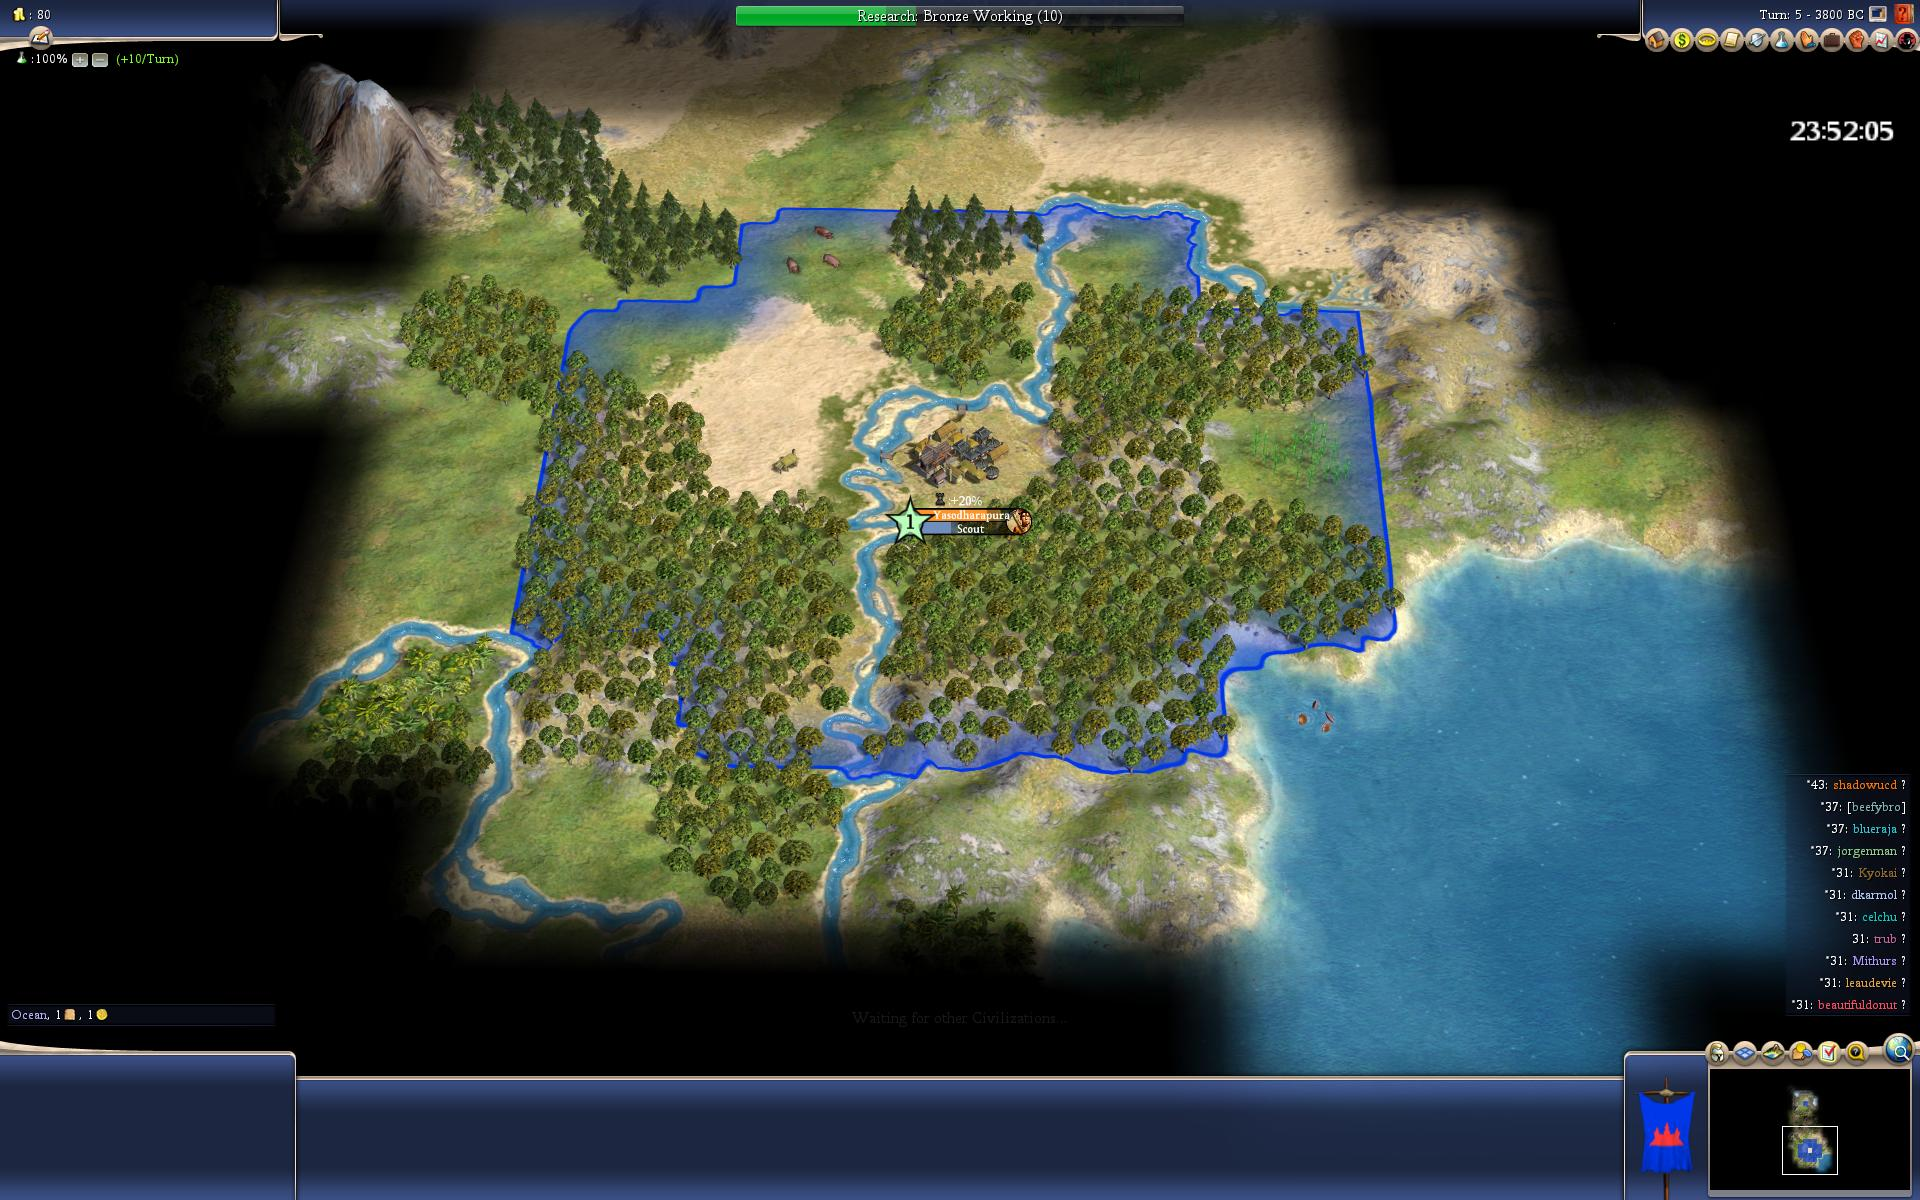
\includegraphics[width=1.0\textwidth]{turn5.JPG}

Those clams are going to be hard to utilize since they're so close to the capital.

Early scouting reveals that I'm near the north-east corner of the
map. There is tundra not-too-far to the north and ocean directly to my
east. Assuming the land is decent, this could be an excellent starting
position since being on the fringes will make it easier to defend
myself.

The first few turns went as well as you could hope. I've already
popped 3 huts, 2 with gold (roughly 40 each) and 1 with animal
husbandry (a tier 2 tech!!). My first scout headed almost due north
and will begin a clockwise scan around the capital. The second scout
will go south and also scan clockwise. Ugh, 4th hut was a map of
tundra and ocean.

Capital is going to be commerce-focussed since it only has 3 hills.

\section*{Turn ~10}

The scout gambit failied terribly. I was able to scout a few jungle
tiles to my south and then I got nailed by a panther (despite being in
a jungle) right before I could pop a hut. My other scout is wounded
and needs to heal up. After he's healed he should probably go down
south of my capital to grab that hut and scout areas closer to my
capital. One thing to note is that I've somehow met Drew but I'm not
sure how; I'm pretty sure I have not seen any of his units. It's
possible he found my borders and then ran into the fog after to avoid
being detected. This is not good on many levels; I was really hoping
Drew would be one of furthest players from me since my bet is that he
is going to play aggressively. I'll have archery soon and I'm already
in slavery, so any super-early rush against me would fail. The copper
city to my east should be city \#1.

Some new developments on the meta game front... Talking to Drew on
steam, something has happened that "if you become privy to it then we
either ally or war; endless at that". I have no idea what this could
possibly mean. I'll have to try to pry some intel from Pat or one of
the other players. It's probably one of the following:
\begin{itemize}
\item Players happening to be very close to each other.
\item Some super-attractive city location (it was this, gem city)
\item Epic random event
\item Some out-of-game event, potentially causing a player to leave the game (with cheese gift?)
\item All made-up meta game
\end{itemize}

\section*{Turn ~20}

Drew and Pat seem to be ostensibly open to peace treaties; I have not
communicated much with any other players. I've bribed Kuan into being
a meta-spy for me and he's been providing semi-valuable information
that indicates a high level of collusion among the players in
752. They are almost certainly cooperating with each other to figure
out where I am. Hopefully, it will end there until people have figured
out where all their neighbors are. Pat reveals that he is very close
to Aaron and is considering an early rush on him. Evidence is mounting
that the map is a bit smaller than hoped.

My other scout is healed and moving towards the hut SW of my capital;
hopefully it's still there (it wasn't).

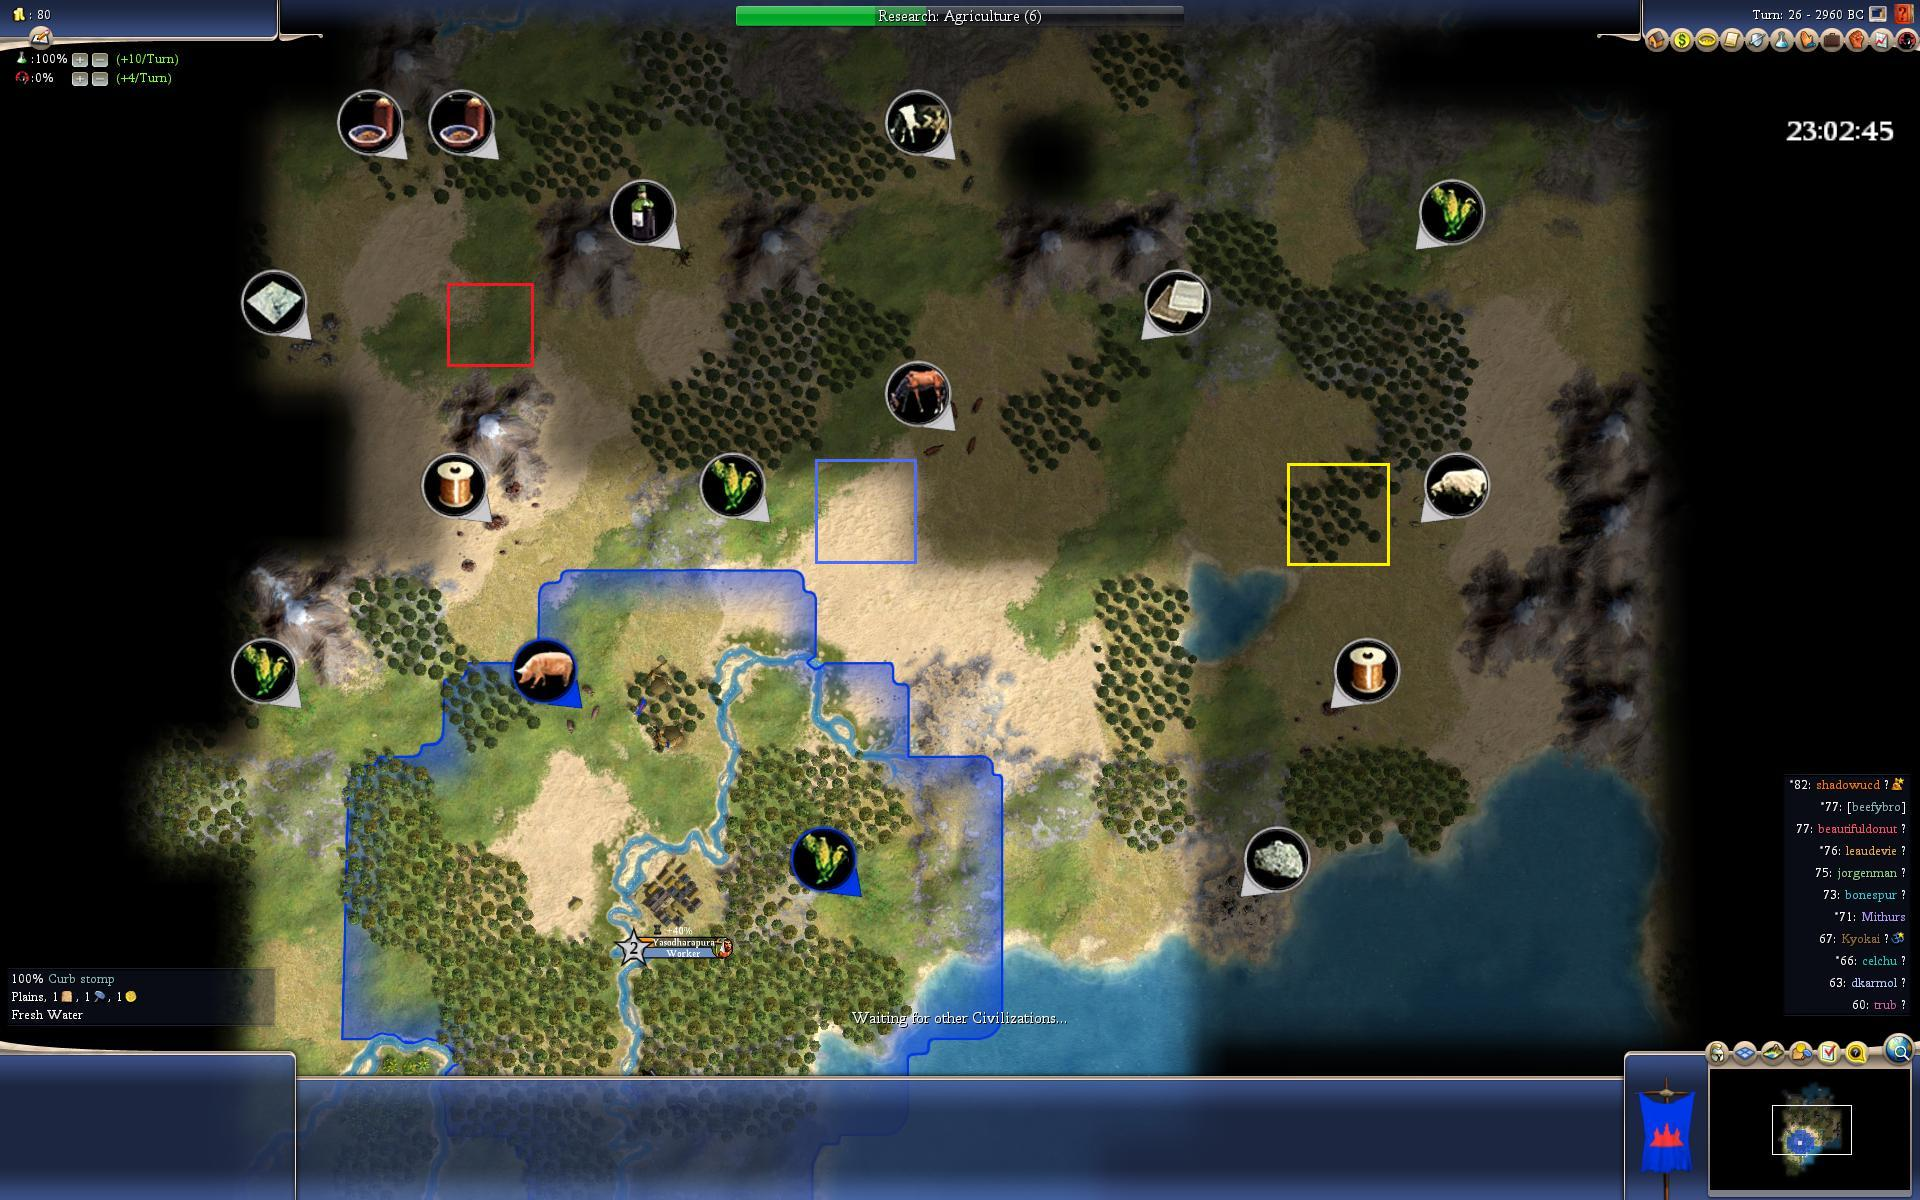
\includegraphics[width=1.0\textwidth]{turn26}

The land immediately N and E of my captial is mediocre but contains
some critical resources. I'm thinking the first city should be the red
square to claim the copper, marble, wine, and spices. With stone to
the east, a strategy focussed on more wonders is possible. The only
solid spot is blue with an abundance of food and some decent
production tiles too. Red has tons of resources but is severely
lacking in food. Yellow could be a decent early-game production/army
city. Ultimately, these choices are fairly underwhelming; hopefully
scouting off to the west will reveal some better spots.

I was thinking, with so many forest, I could go with a super-worker
gambit and make 3 early workers instead of two. In my testing, this
delays the first city by several turns, but you might have 2 extra
cities by 0 AD (you actually have to watch out for over-expansion with
this opener). The key issue will be if there's a city spot that looks
contested; unfortunately, my scouting has been so weak that I just
don't have enough information yet to make these hard choices.

\section*{Turn 33}

The super-worker gambit is complete with my 3rd worker just
produced. The idea for the third worker will be chopping, building
roads to new cities, helping new cities to get going, then on to the
next new city.

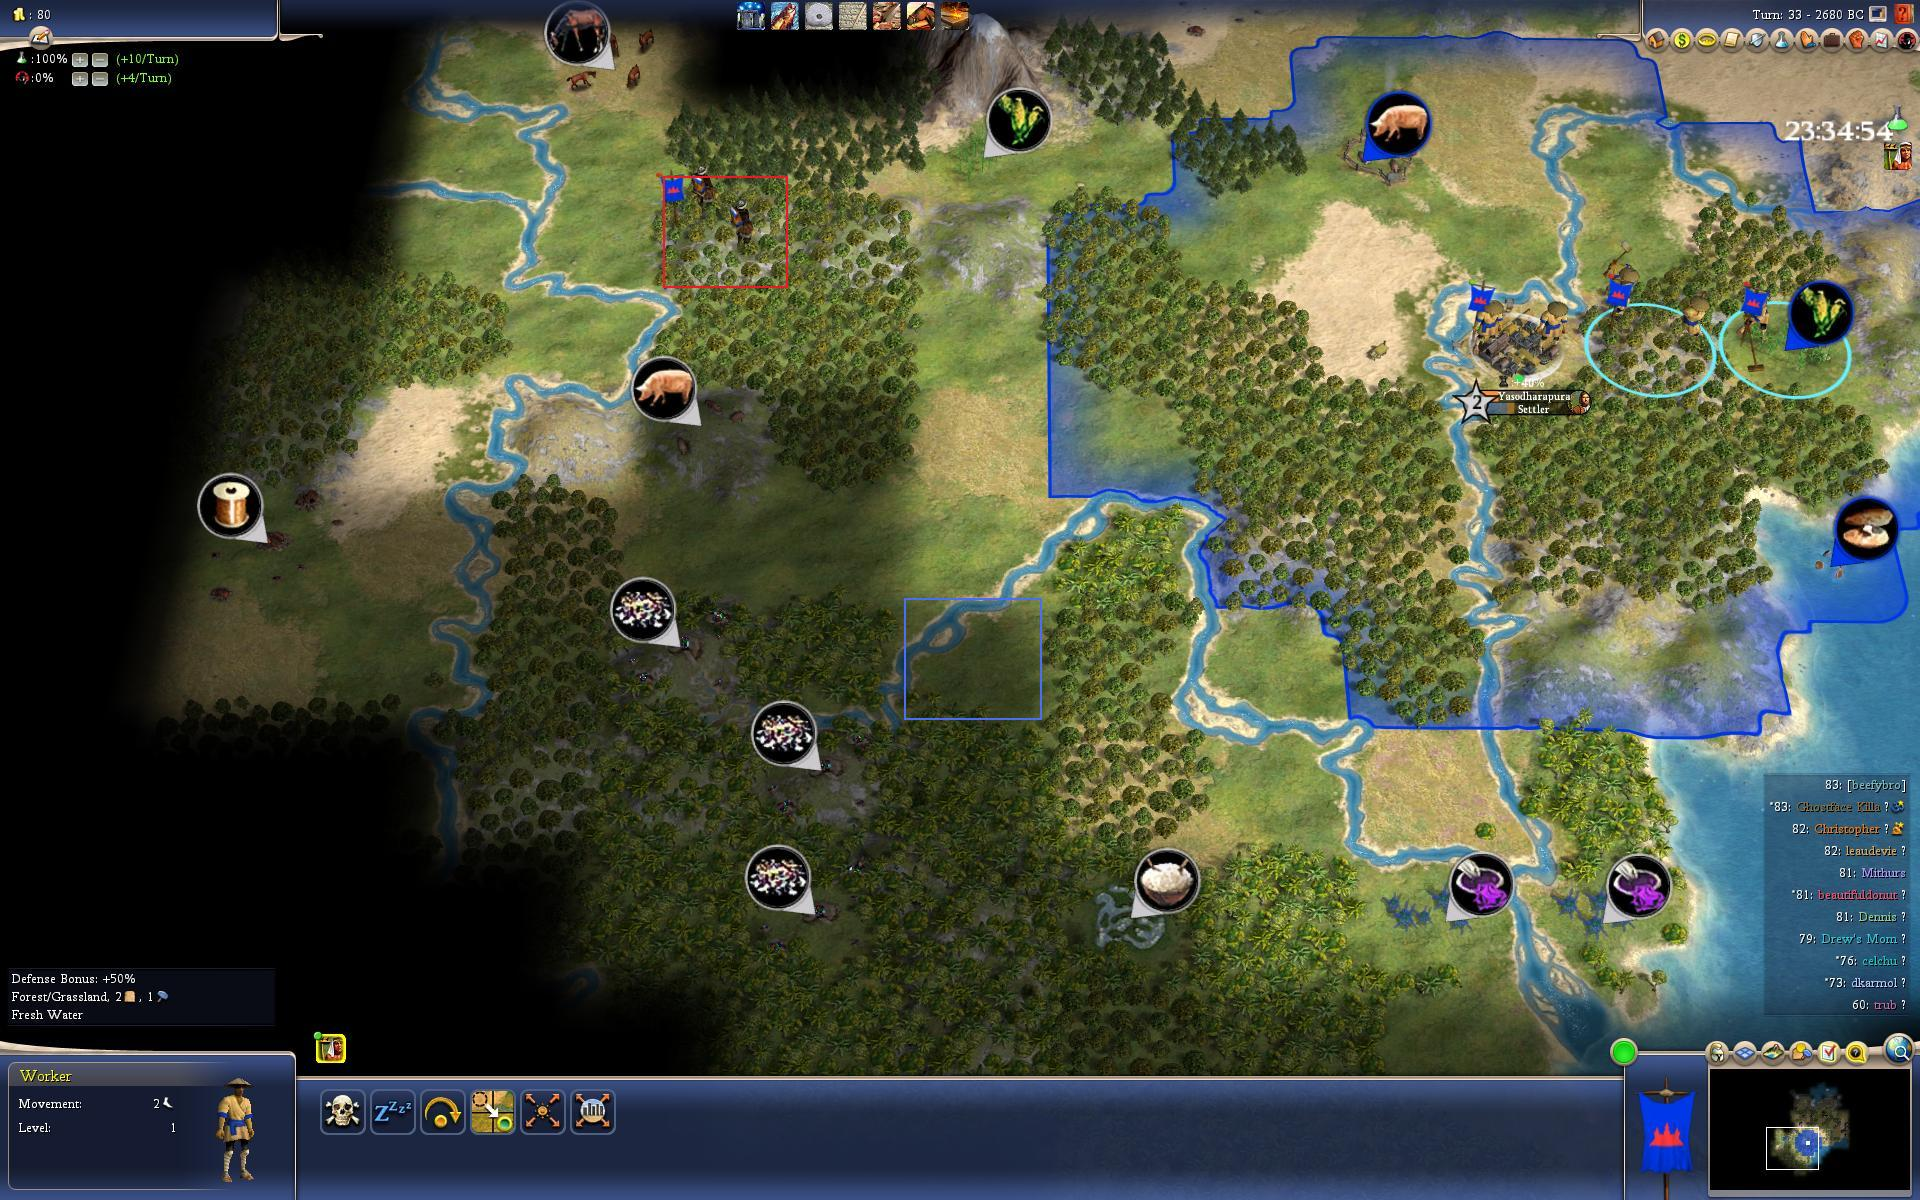
\includegraphics[width=1.0\textwidth]{turn33}

More importantly, my remaining scout has found some very good land off
to my immediate west. Drew knows about this land and it seems likely
that there will be a fight for it unless I can perform some good
diplomacy. Drew has hinted that there may be multiple players vying
for control of this land, but I haven't met anyone else yet. While
dangerous, I feel that I need to stake a claim in this area if I'm
going to have any chance to win. The red square will be my first city
in order to claim excellent land plus horses. It will be tempting to
make the blue city the second city since it will be amazing. The safer
choice would be to get a bronze city up. The red city is a little
agressive, but it's BFC is one tile from touching the BFC of my
capital, so it's hard to say that it's an unjust placement.

\section*{Turn 36}

I've decided that there can't be peace between Drew and I. I'm going
to pretend to let him have the good land to the west while I chop out
an army. My first city will be the copper/production city to the
east. Third city will be horse/commerce city to the north. I'll go in
heavy and hit his city \#2, which should take out his copper and
horses. Hopefully this will give me the momentum I need to finish him
off. I don't think I can wait until cats. Scout \#2 died to a massive
bear mauling; bleh.

\section*{Turn 40}

Drew has settled 1 west of my red city. The attack will be here.

\section*{Turn 45}

Second city founded at the decent copper site in the east. It should
be a decent early production city. I'm starting to question whether
war is the right path. If I can get the gems city and a few other OK
spots, I could probably get to 7+ cities. This is a hard
call. Fighting and winning a war against Drew would almost guarantee a
pile.

\section*{Turn 55}

I've decided to leave Drew alone for now. Demographics indicate that
I'm doing fairly well, \#1 in production and land area, \#2 in food. The
next hard decision is what tech to get next. I believe that gems can
help keep my economy humming while I over-expand; the problem is that
iron working is going to take 21 turns to research at 100\%. My gold
will probably run out in about 6 turns once my 4th city (gem city) is
placed. This would leave me with nothing useful to build in any of my
cities, except for granaries, for quite a while. I need to start
getting cottages down immediately and make sure that cities are
focussing on commerce. I also need to get a couple chariots out to do
some better scouting.

\section*{Turn 57}

Very unfortunate: Drew has settled 1W of the top gem, meaning it will
be very difficult to capture that gem within my borders and much
harder to keep the peace. I still settled in the original planned
location; culture should allow me to gain the upper hand in this area
early on. Drew was enraged and renamed his gem city \verb|with stupid ->|.

It looks like Lynda is my eastern neighbor, yikes.

\section*{Turn 58}

Drew has made it clear to me that peace between us is impossible. Here
is the plan: Angkor Wat will pop it's borders before Drew's nearby
city, giving me line-of-sight and easy attack on that city. Since
connecting my bronze is going to take too long, I'm going to have to
use chariots. The extra movement point will be very nice in the
upcoming surprise attack. The idea will be to mass-up chariots and
leave them sitting at the red square. Once it looks like I have a
decisive advantage, they will strike, hopefully taking roads so that
they can hit on the same turn as the declare.

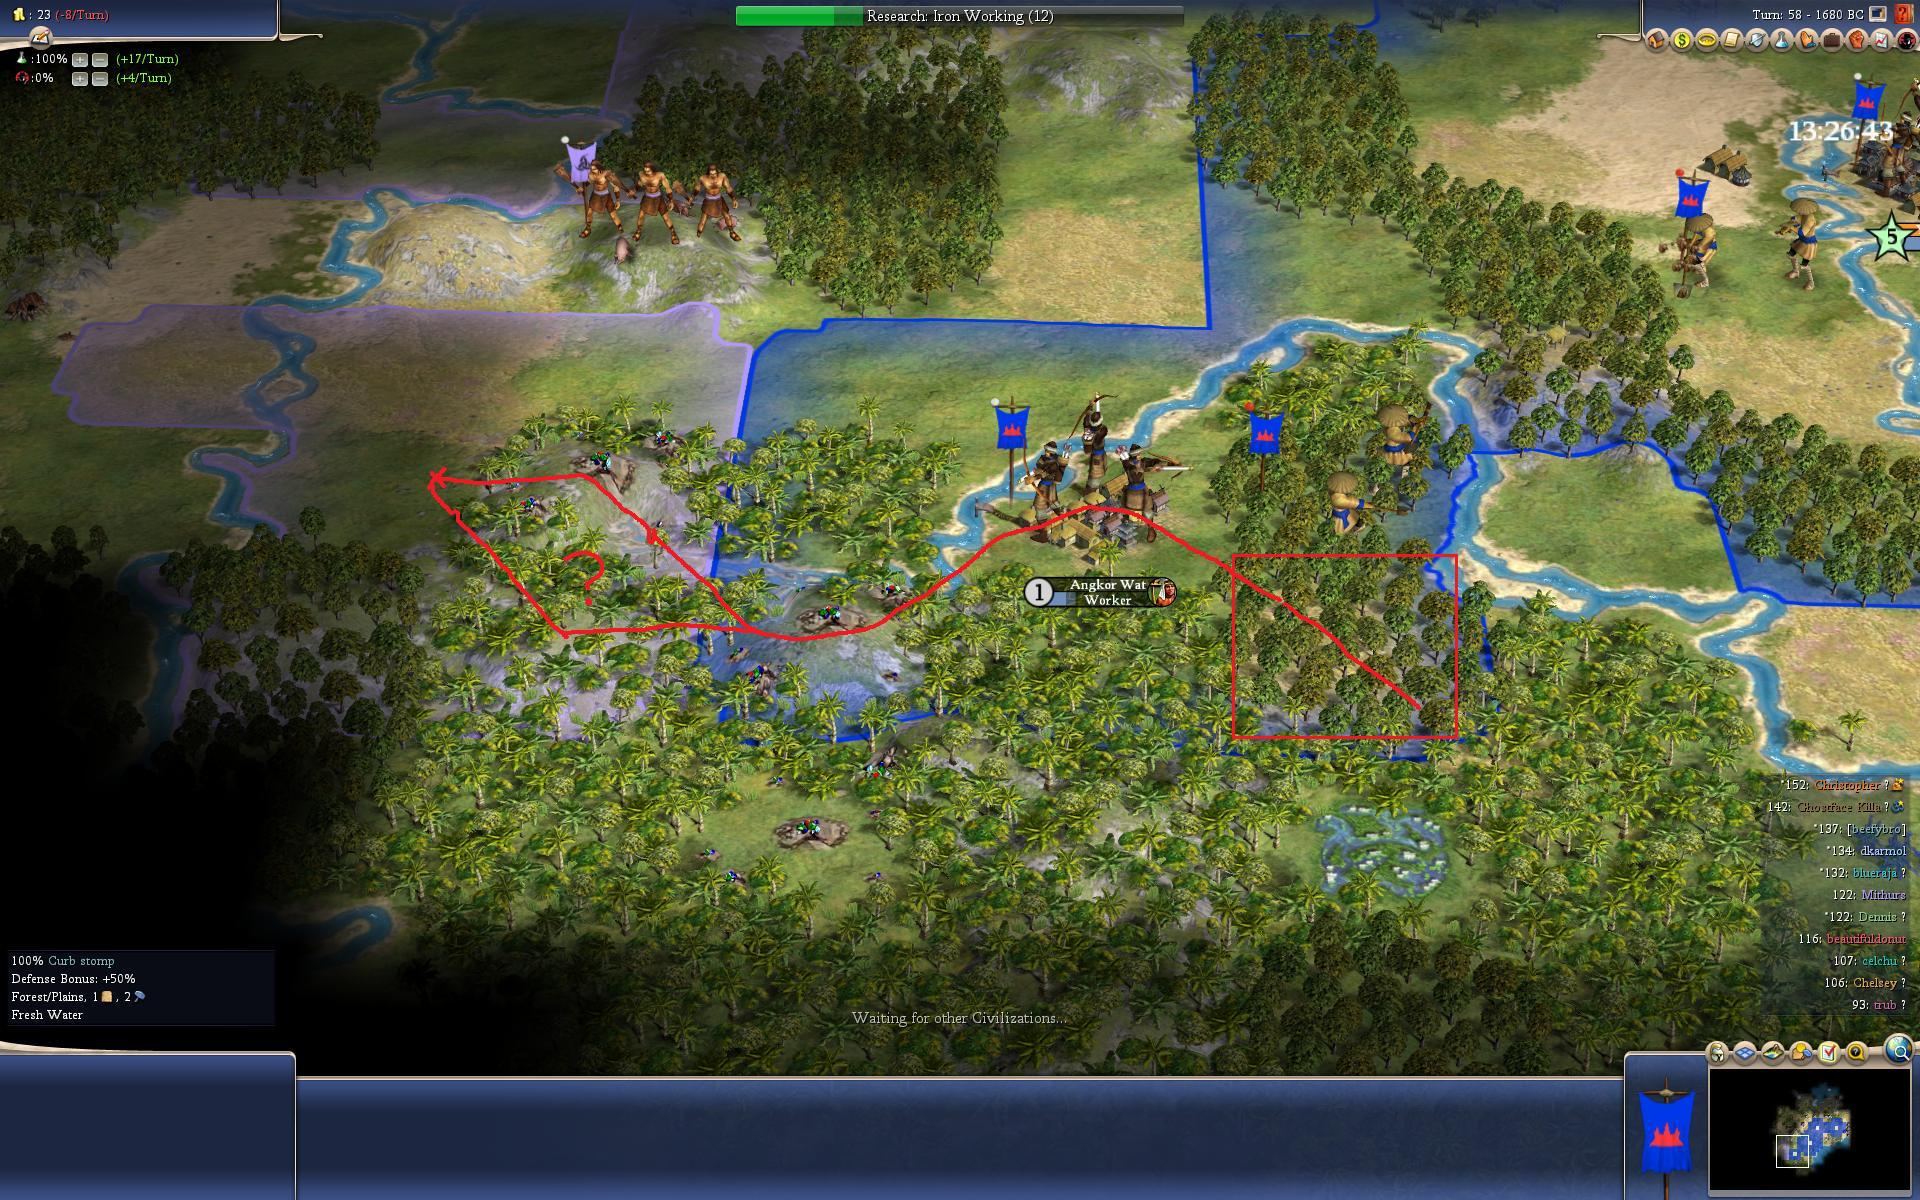
\includegraphics[width=1.0\textwidth]{turn58}

Roads will need to be built without giving the attack away or tempting
Drew to steal a worker. Note that this window will open up in 6 turns
and will not stay open long. Probably 10 turns. I'll be lucky to have
2 chariots ready by then. I should probably start chopping the capital
again soon.

It should be noted that capturing this city should deprive drew of
copper, allowing me to overwhelm him with metal units to finish
him. I'll have to be sure to go heavy on spearmen since horses will be
his only strategic resource. Drew thinks I'm weak militarily, so
hopefully this will come as a complete surprise.

Demographically, things are going well, especially land area:

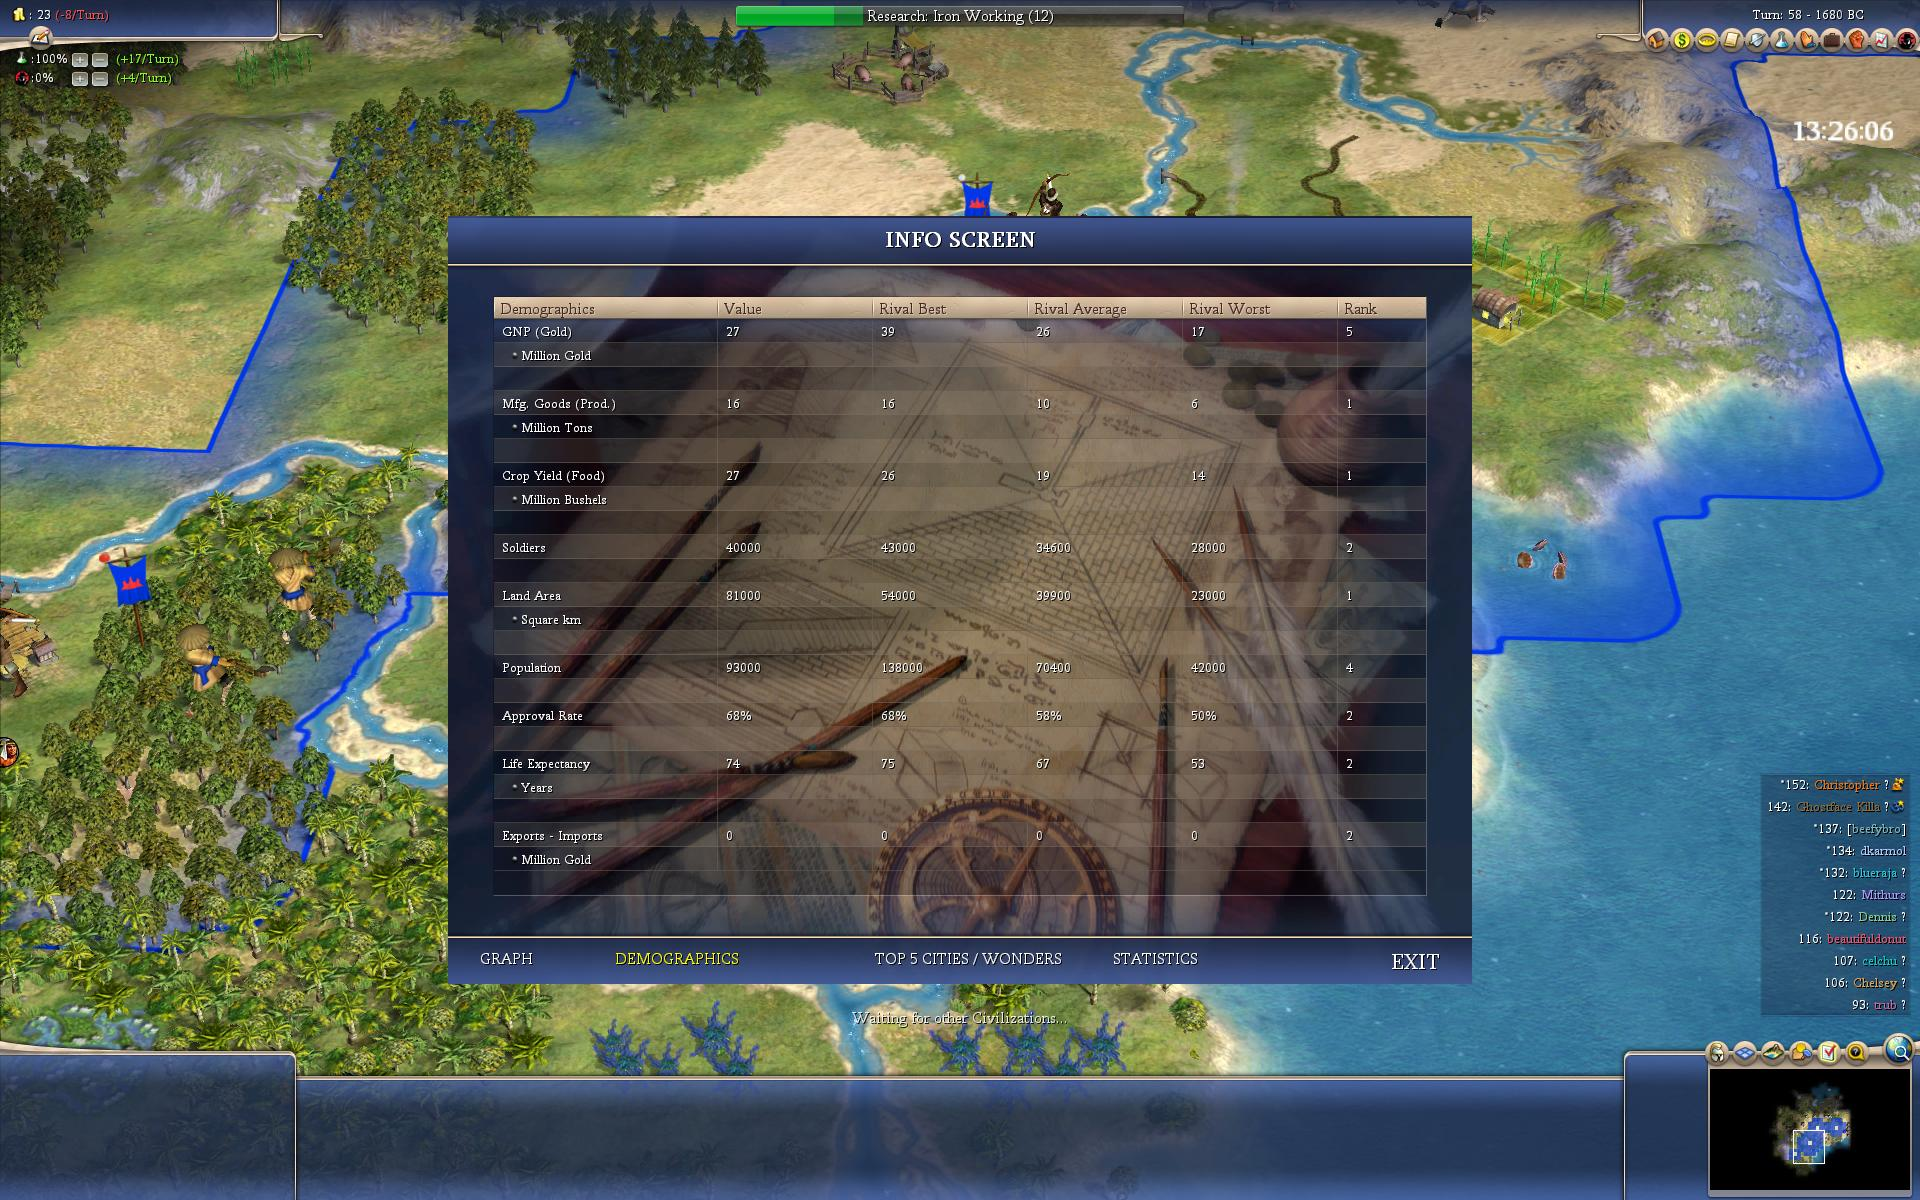
\includegraphics[width=1.0\textwidth]{turn58-2}

\section*{Turns 60-67}

War with Drew. When I moved my worker over to the gem west of town, I
sent an archer with him just to be sure Drew wouldn't be tempted by
the worker steal. Drew correctly deduced that this movement meant two
things: Ankor Wat was undefended and my archer had lost his
fortification bonus. Since Drew had several warriors in the area, he
thought that he may have a chance at taking the city. In hindsight,
moving this archer was a mistake since I would have seen any potential
worker steal coming 1 turn in advance. It goes without saying that any
chance for longterm peace between Drew and I is gone.

The ensuing war was not helpful, but neither side took serious
losses. I whipped an archer in my capital and it promptly lost an 85\%
battle to one of Drew's warriors. Fortunately, I was able to connect
my horses and kill a warrior with an archer. Ankor Wat was saved by
the archer's +50\% city defense attribute which scared Drew off. This
was lucky; I think the smarter play would be to sacrafice a warrior
just to see how much damage it could do to the archer, if serious
damage was done, this would give him a good chance of taking the city
with the second warrior.

\section*{Turn 67}

Peace with Drew. I think getting chariots out slightly before him
scared him into peace. I wonder if he realized how dangerous his
position at "With stupid" was after the border pop of Ankor Wat,
giving me full visibility of city (only protected by a single warrior,
but other troops in the area). Accepting peace was the hardest
decision of the game so far; I think my 2 chariots probably could have
taken the city, but it would be a huge gamble. I decided to opt for
peace, hopefully luring Drew into false sense of security. This peace
treaty means I cannot attack until turn 78.

\section*{Turns 68-77}

Build-up to war!

Rationale: Having Ankor be at max effectiveness (harvesting all 3
gems) is key to my strategy. My economy is weak and I need a large
boost in commerce to keep up with the financials and allow for further
expansion. "With stupid" simply has to be destroyed. What's more, I
believe "stupid" is Drew's only source of copper, so losing this city
potentially allows me to conquer him entirely.

A well-balanced army is being assembled at the red square, keeping the
units out of Drew's line of sight. By turn 77, I need to build a road
on the purple square and have the stack on that square. The road
network will allow me to get to the blue square with one move once war
is declared. It seems very hard to believe that drew will have enough
units in the city to defend it.

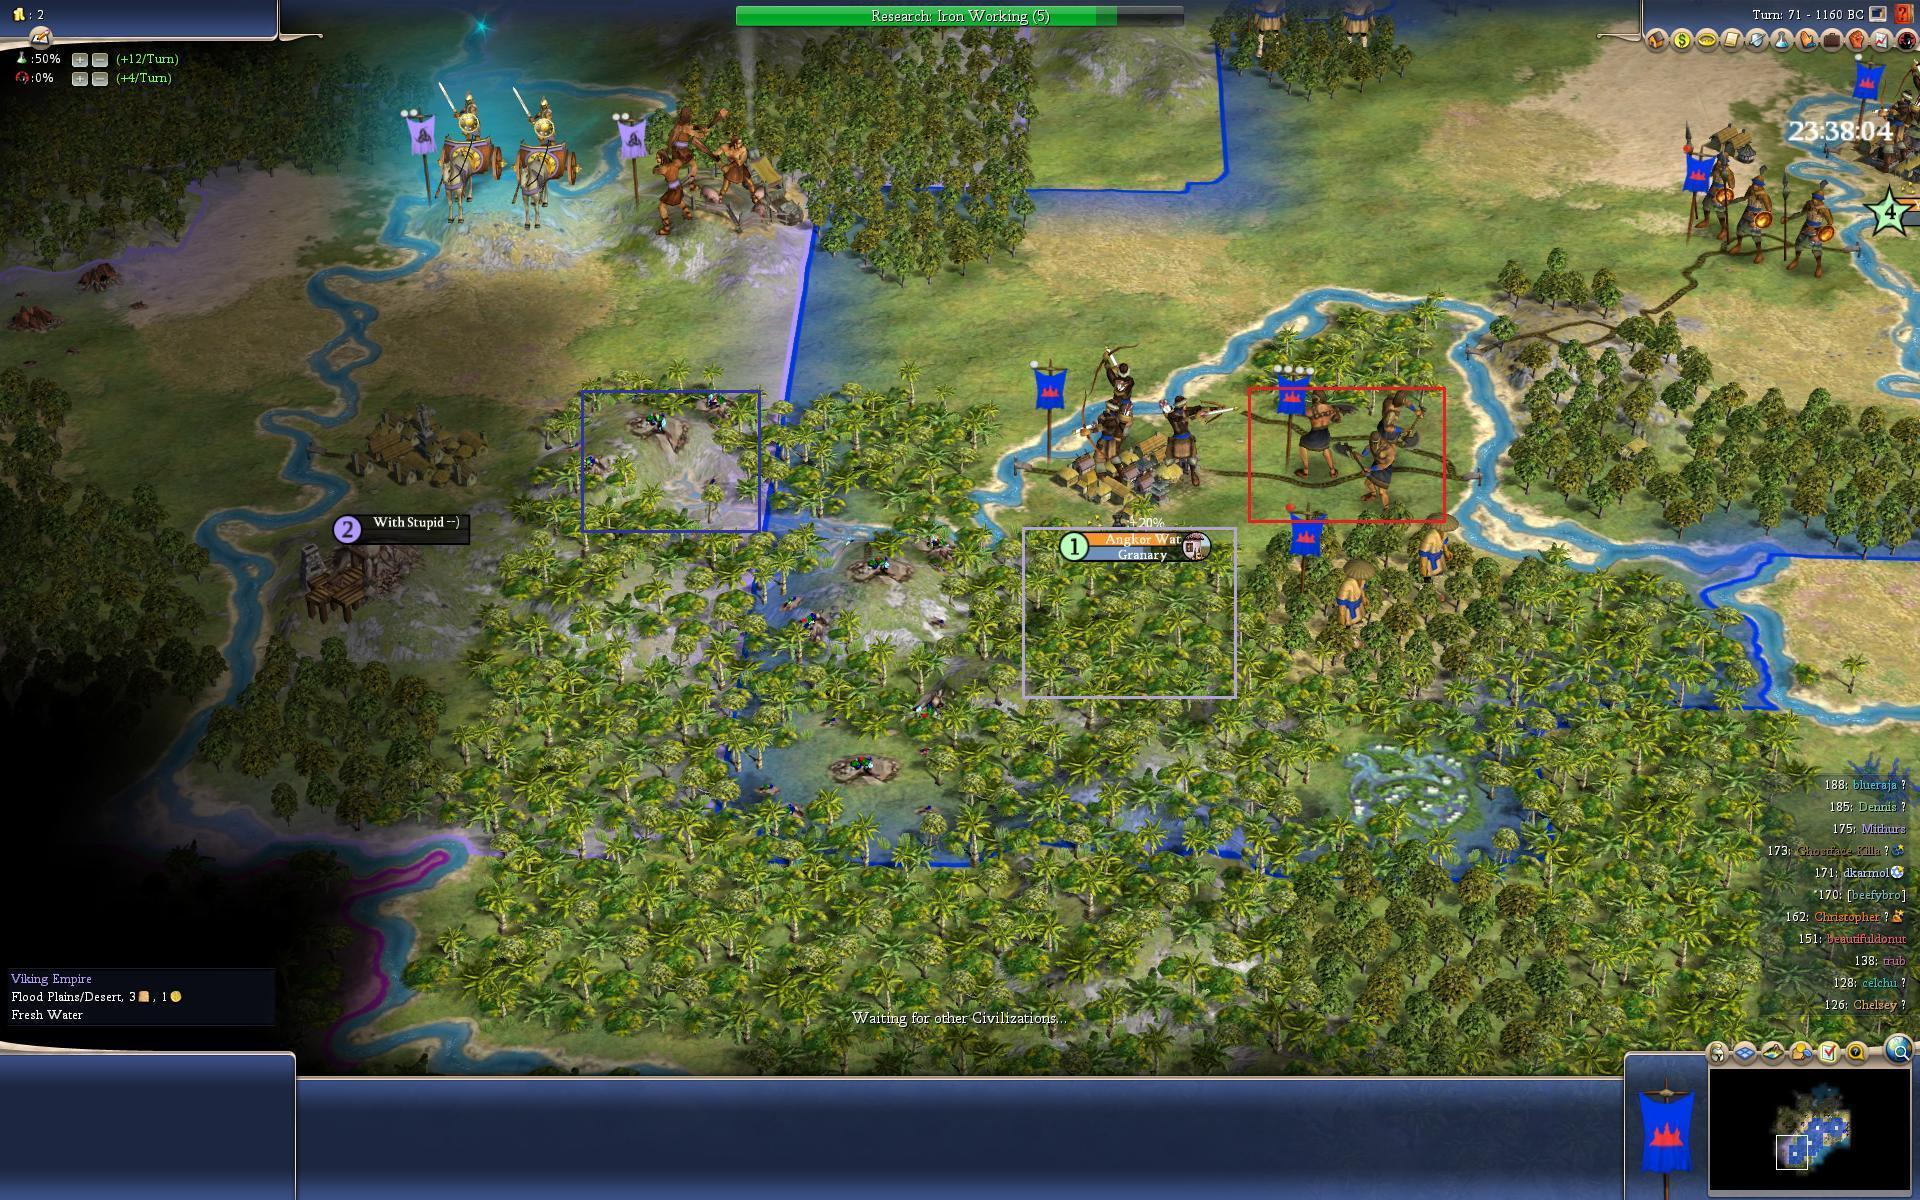
\includegraphics[width=1.0\textwidth]{turn71}

There are a number of things working in my favor here:

* Element of surprise. I've tried to keep up the ruse of peaceful meta
game to keep drew from feeling threatened. Also, Drew thinks that the
copper node to the north west of my capital is my only copper source
and therefore I do not have metal connected yet, making me not much of
a threat.

* Superior army. Drew's copper node is 2 west of "stupid". Drew's
borders only just expanded to encompass this copper last turn and
he'll need to build two roads to connect it. This should leave him
without metal until just before the war starts. At this point, I
should have 4-5 metal units. I also have lots of reason to believe I'm
sinking more production into military that Drew is; he's probably
working on his libraries at the moment.

* Drew is still not in slavery, making it harder for him to whip a
panic army.

Unfortunately, the power graph is going to give me away very soon; I
can only hope that Drew won't have time to react. The demographics are
already of the verge of giving me away.

Dave Cop's borders have come into view near Ankor. When I declare on
Drew, I'm going to open diplomacy with Dave; I will offer to burn
instead of capture Drew's cities in exchange for assistence or at
least non-intervention on his part. This will open up land to his
north for settlement.

\section*{Turn 73}

I am almost 100\% certain that my attack is going to catch Drew
completely off guard. The only problem now is the diplomatic
situation. Dave K is not happy with me to my east. Lynda is supposedly
making a large army. And Dave C is talking about all the axemen he has
and a supposed alliance with Drew.

I am going to open up diplomacy with Lynda to see if she's open to any kind of agreements.

\section*{Turn 74}

Lynda appears to be open to some kind of agreement against Karmol, but
she hasn't gotten back to me yet.

Drew and I have agreed to reduce the spying on each other so that we
can put points into other players. He doesn't know that I don't want
to spy on him because I don't think he's going to survive the upcoming
war.

Demographics show that my military is 50\% bigger than anyone
else's. My economy is poor however... need to get those gems online
ASAP now that I have iron working.

Unfortunately, the discovery of iron working has really rocketed my
score and players are starting to notice. The diplo situation could
get ugly in a hurry.

\section*{Turn 77}

Attack!! The initial attack shows exactly what I hoped for; Drew is
caught completely off guard and still has a mere warrior defending
"stupid", so that city is mine for sure. This will limit Drew to
producing archers and chariots, so I'll need more spearmen for
sure. Drew was initially so demorilized that he retired from the game;
after a few minutes he reconsidered and rejoined.

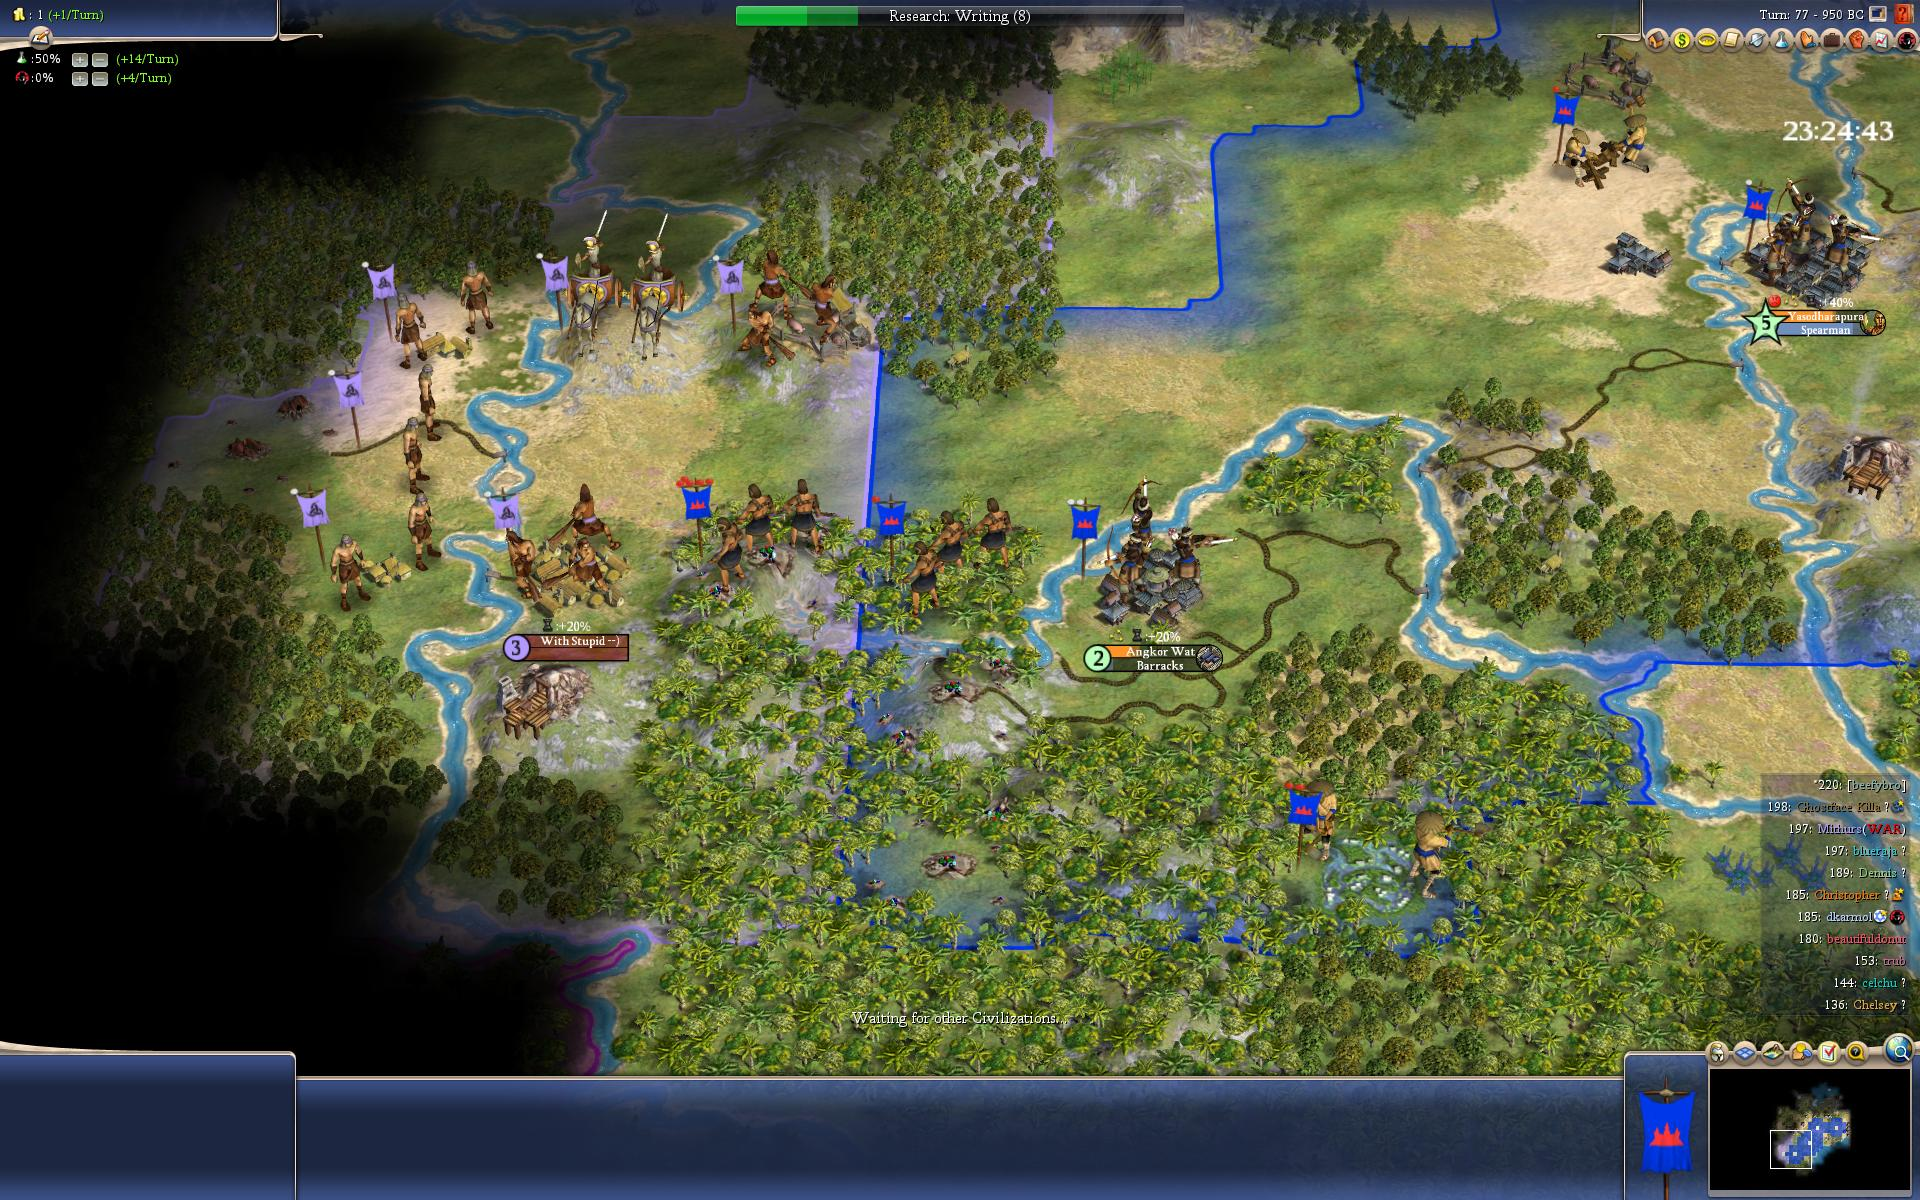
\includegraphics[width=1.0\textwidth]{turn77}

The trick now is knocking Drew out of the game without other players
getting involved. I've emailed some proposals to Dave to see if I can
keep him out of the fight. Assuming these work, the only problem is
Karmol.

As a side note, Drew is in utter disbelief (to the point of raising
the possibility that I somehow cheated!) as to how much production
I've turned out at this point in the game. This confirms the strength
of creative/expansive and early chopping. I saved a lot of hammers on
cheaper workers, not having to build monuments, and cheaper
granaries. Combine that with the mega-worker gambit, massive chopping,
and a capital that was surrounded by forest, and you end up way ahead
in production.

\section*{Turn 78}

Drew retreated his units out of "stupid" (wisely) and the city was
taken without a fight, giving me 40g. Next up is the horse/pig city to
the north.

Hopefully Drew won't get archers anytime soon.

On the diplomatic front, Lynda has agreed to a 50-turn defensive
alliance against Dave K. Dave C has agreed to stay out of the war with
Drew in return for a guarantee that I raze "stupid", giving him some
breathing room to the south. These are very positive developments. A
big attack by any player would probably save Drew since it would force
me to retreat my units for defense.

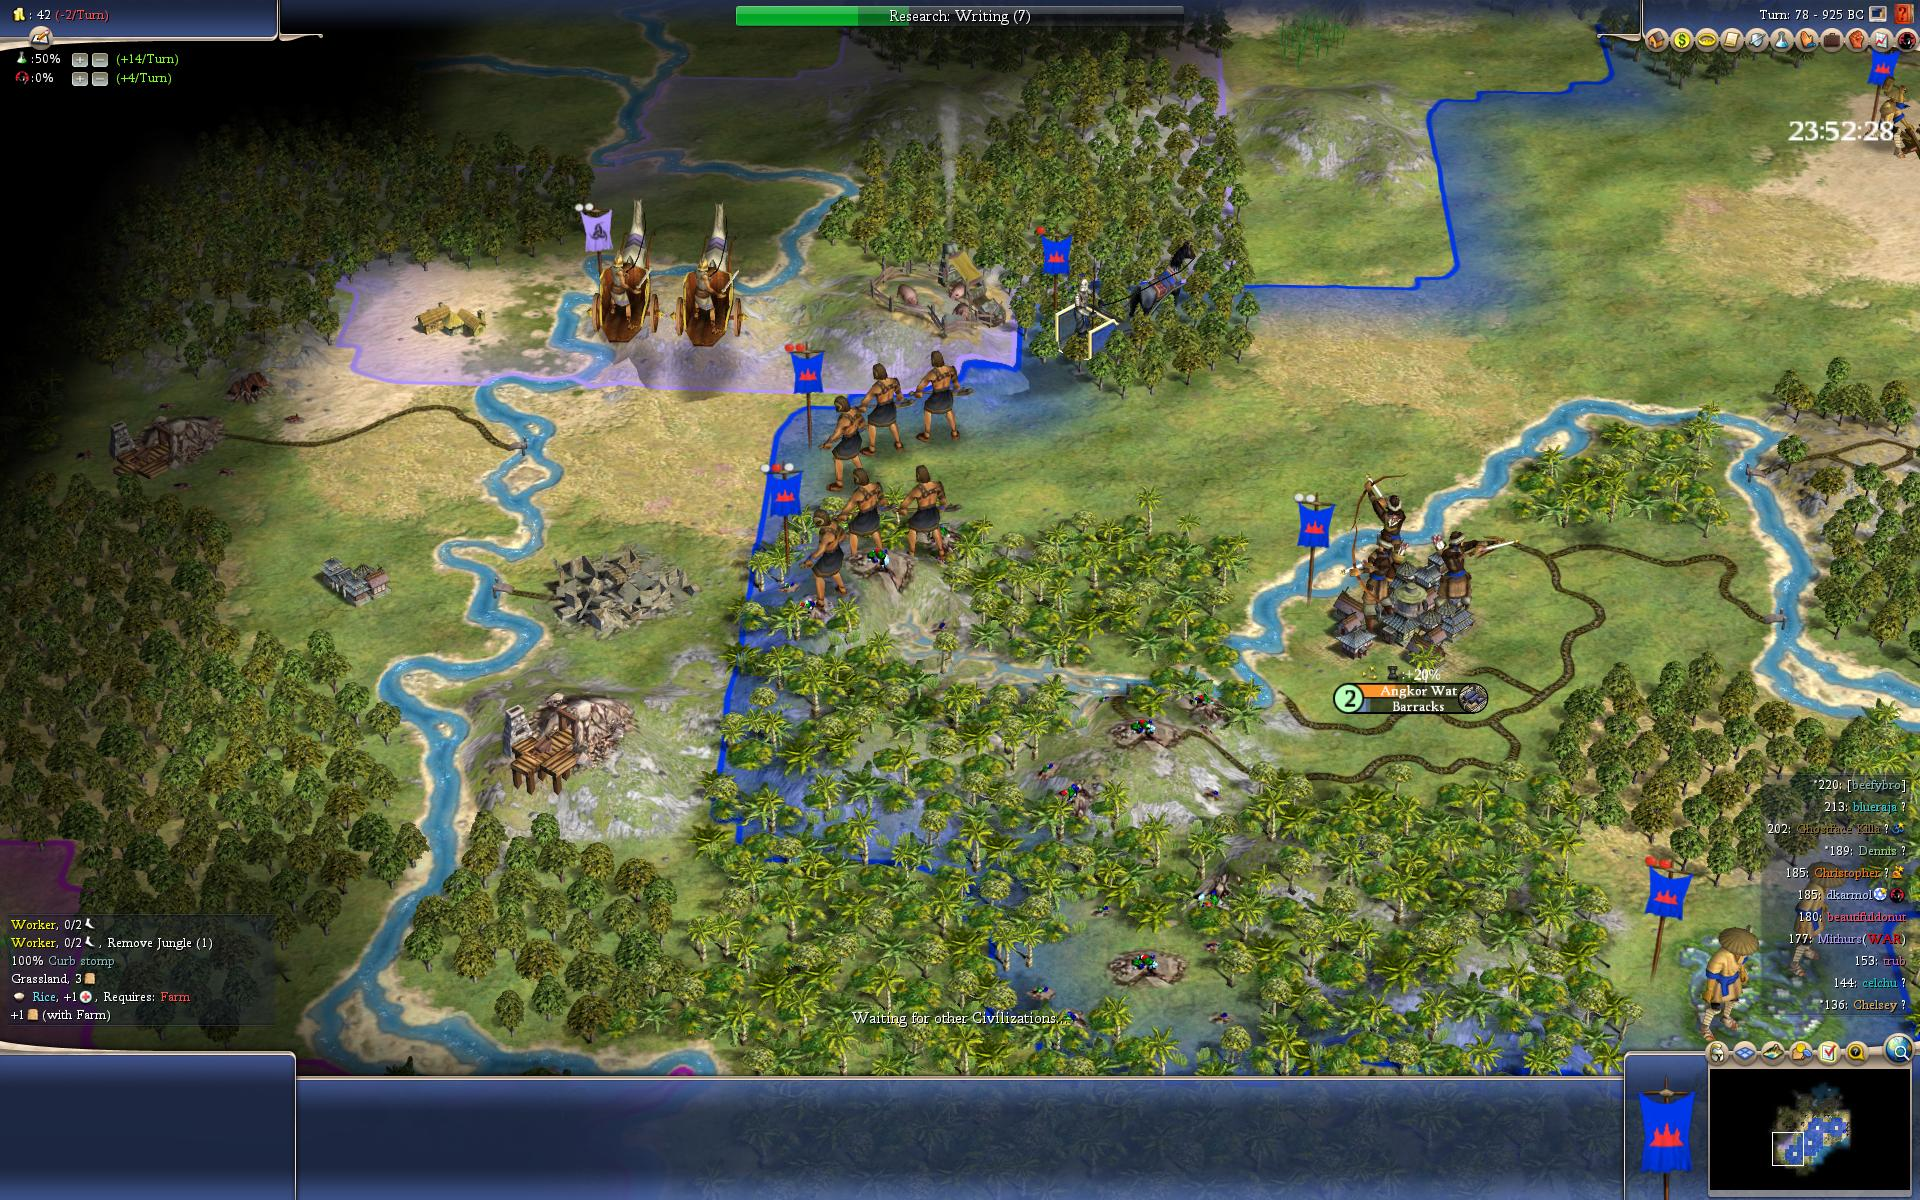
\includegraphics[width=1.0\textwidth]{turn78}

\section*{Turn 79}

Drew has 2 chariots and 3 warriors defending the city. My chariots
seem to be the least useful unit I have in my stack, so I will
sacrafice them, at 50/50 odds +5\% withdraw chance to weaken the
chariot defenders. Then I will attack with the city raider axeman to
take out the last chariot. Then all that remain are warriors. I should
probably attack with the spearman as well, since the spearmen will be
less useful once he starts to make archers.

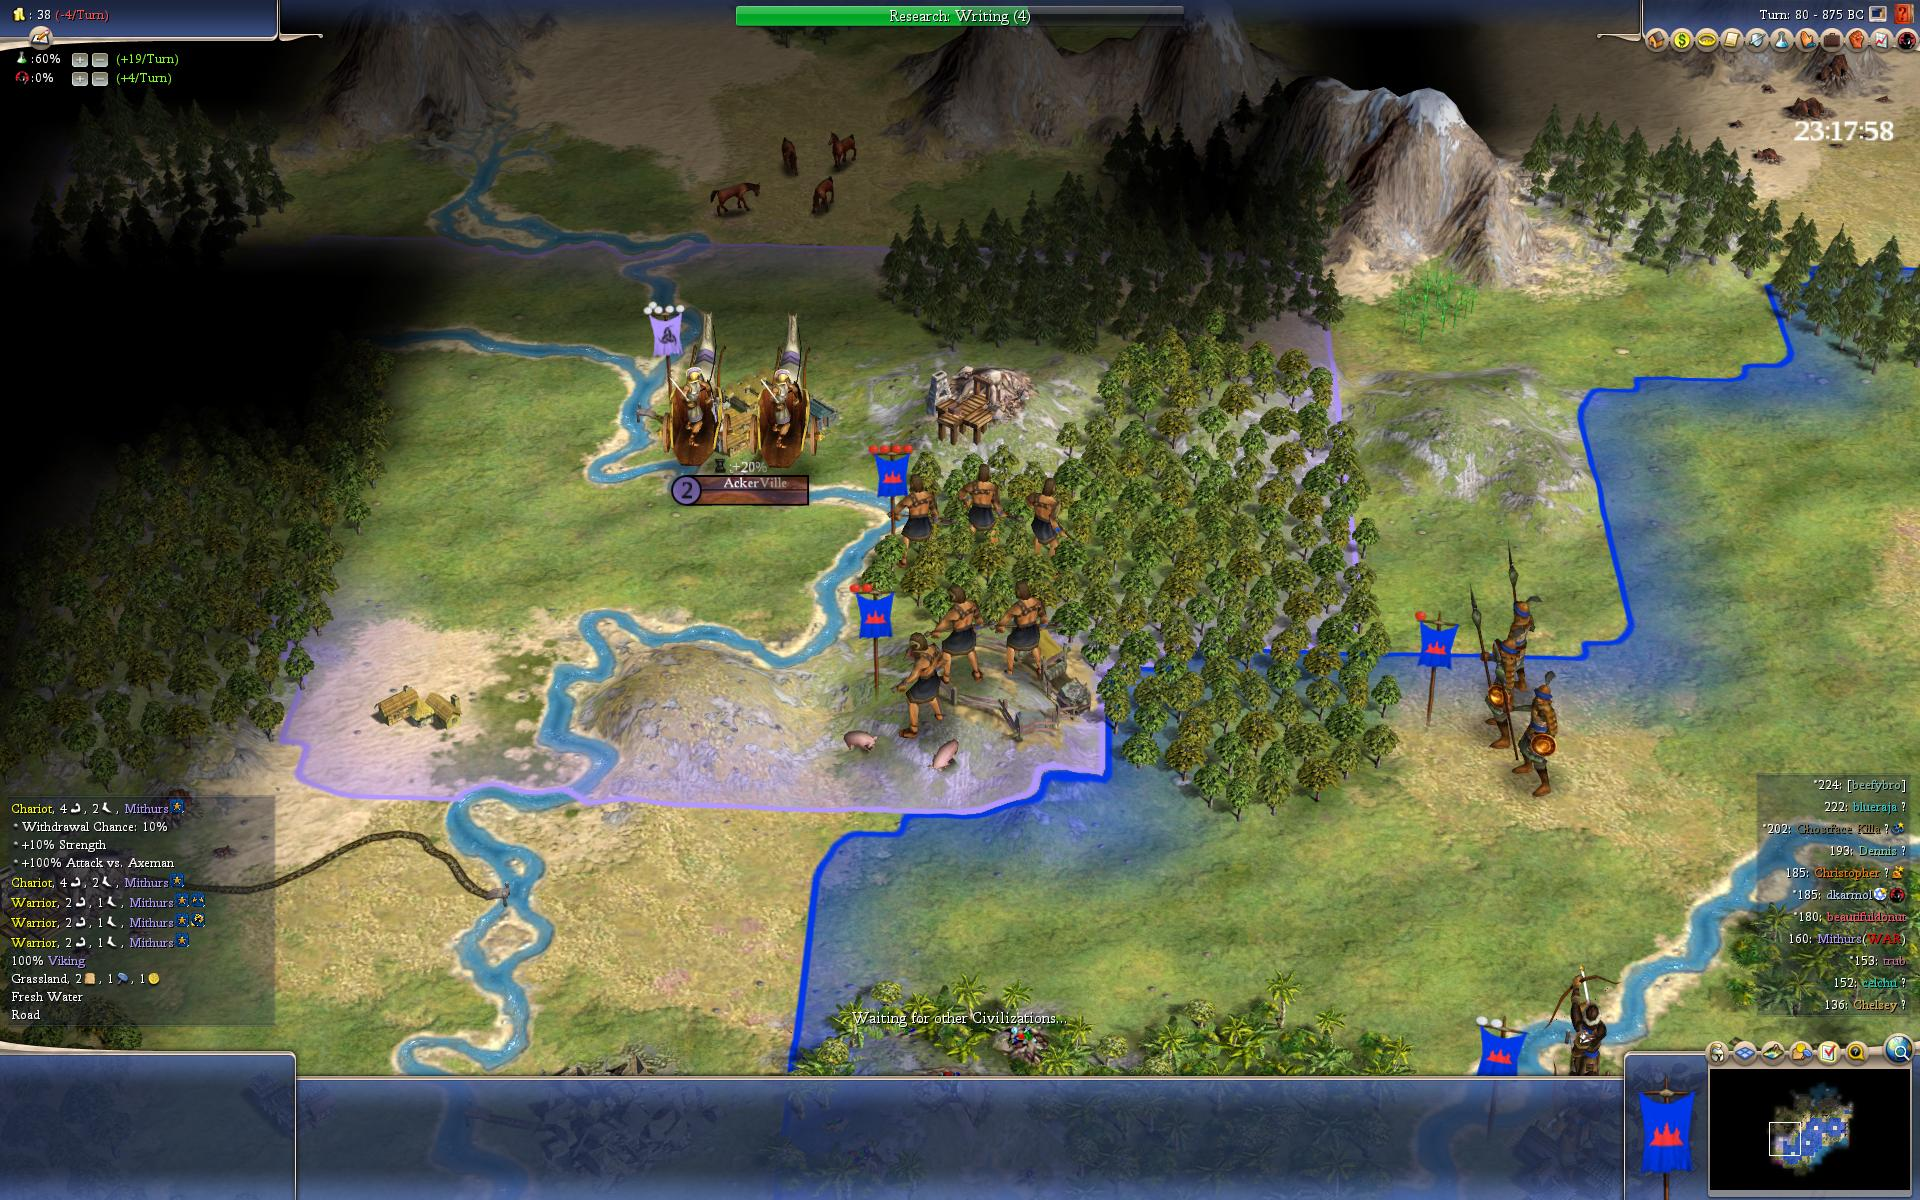
\includegraphics[width=1.0\textwidth]{turn79}

This is going to be closer than I'd like.

\section*{Turn 80}

Drew whipped a chariot and moved an additional chariot into the city,
putting him up to 4 chariots and 3 warriors. He supposedly has archers
next turn, so I probably won't be able to take the city with this
current force. I could stay and pillage, but it's probably now best to
end the war. Drew and I have agreed to an asymmetric NAP; 50 turns for
me, 100 turns for him; so he won't have the option of attacking me for
quite a while. This is a pretty good deal and I don't feel like the
war was a waste. My fear is that Drew will plop a city down in the
same spot as before, so the culture of Ankor Wat need to be a high
priority to discourage this.

So the next big issue is where the next city should go. There are 3 possible spots:

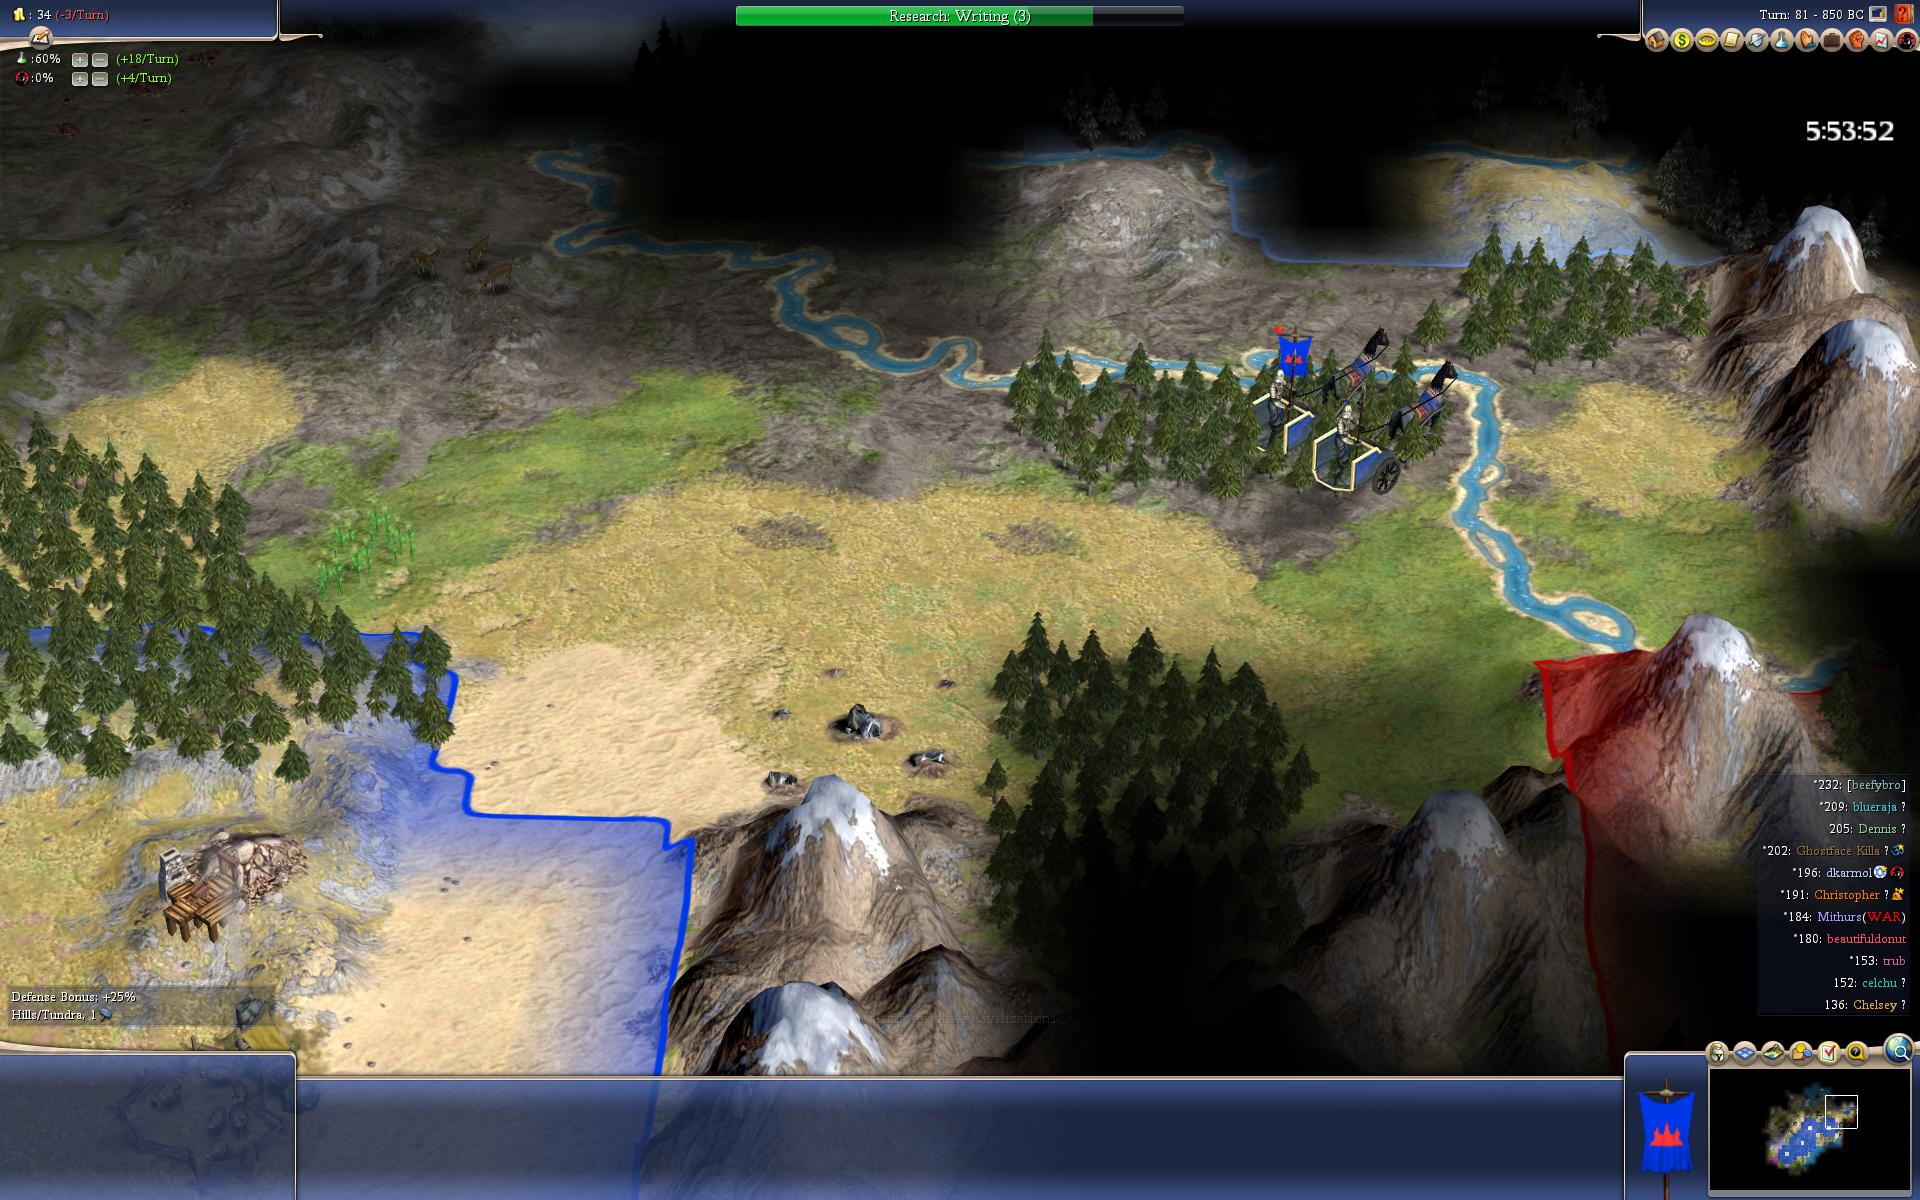
\includegraphics[width=1.0\textwidth]{turn80-1}
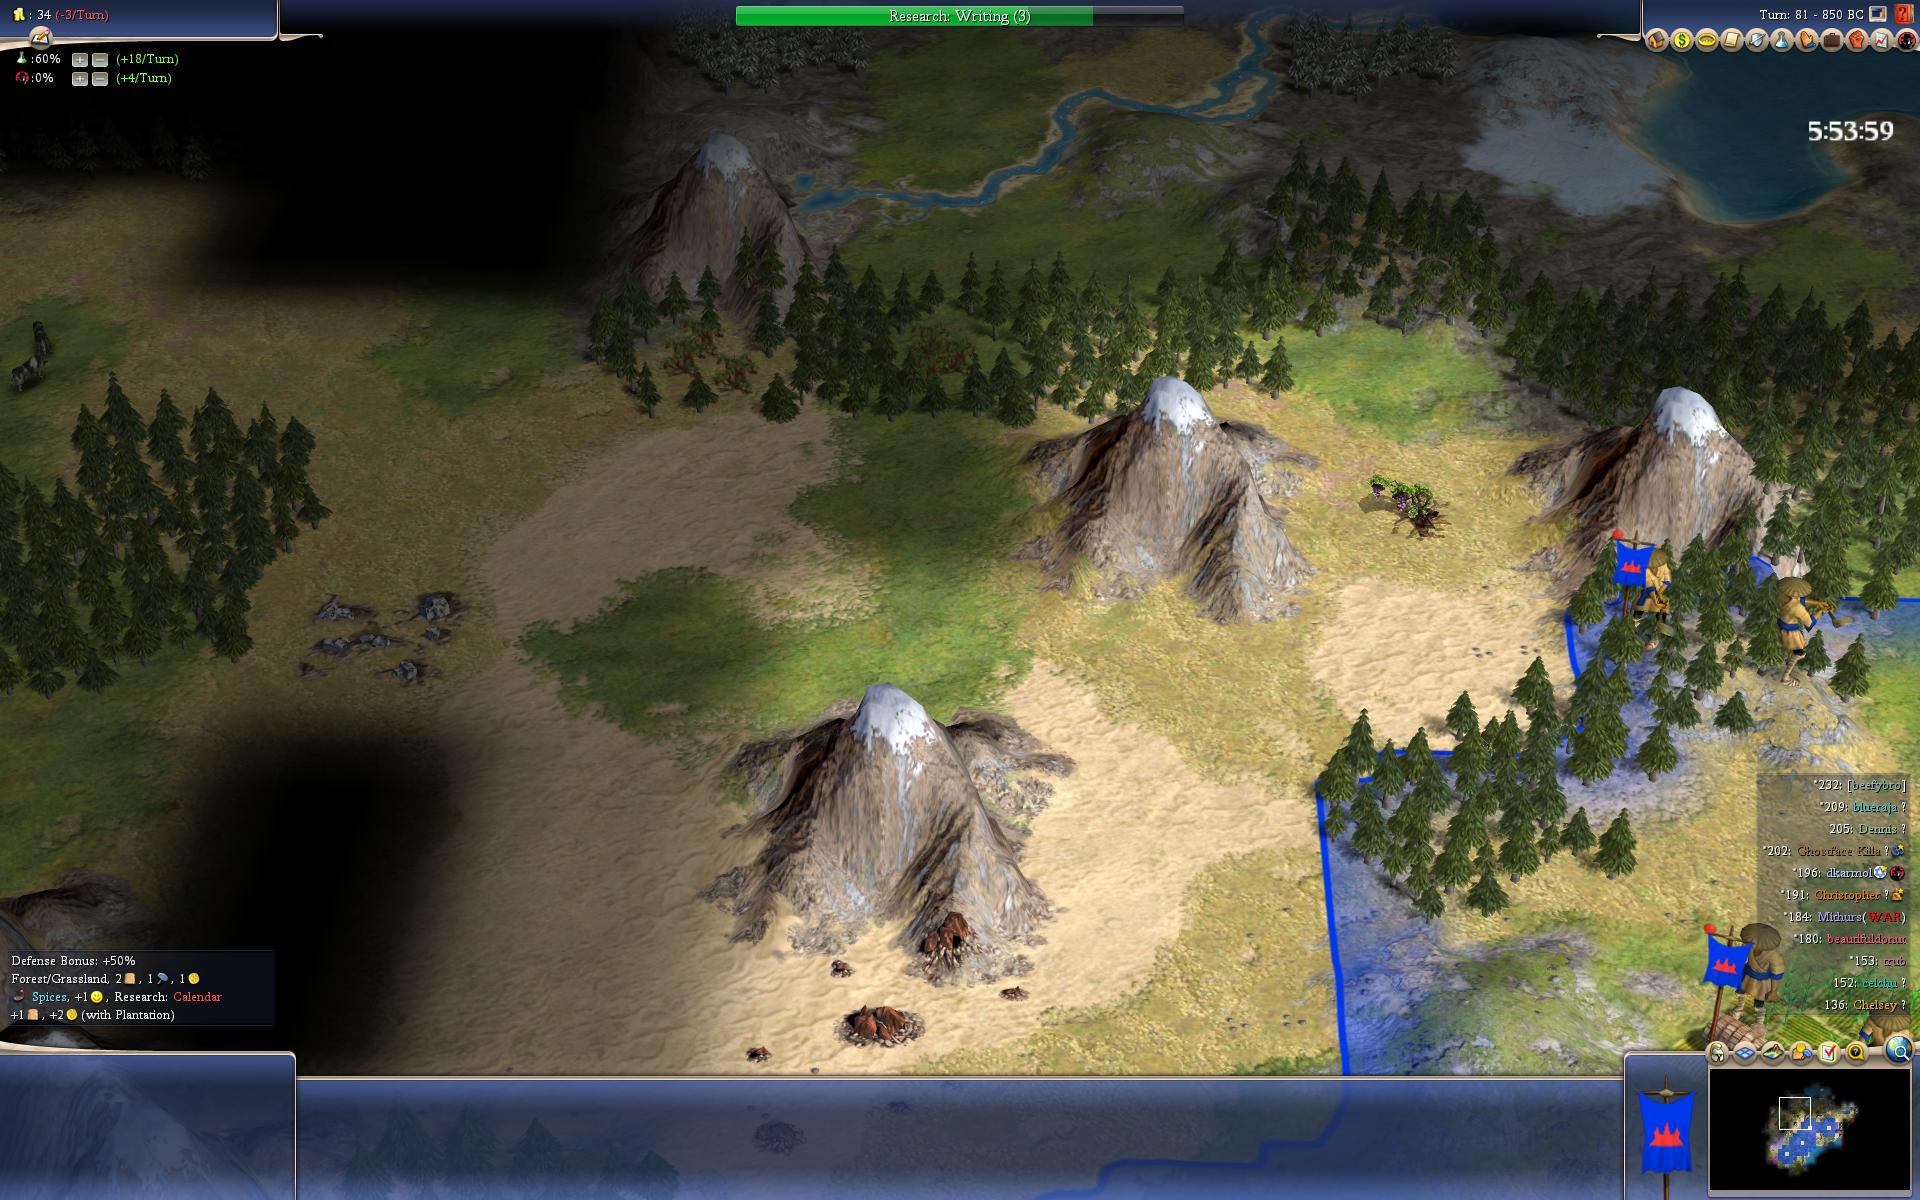
\includegraphics[width=1.0\textwidth]{turn80-2}
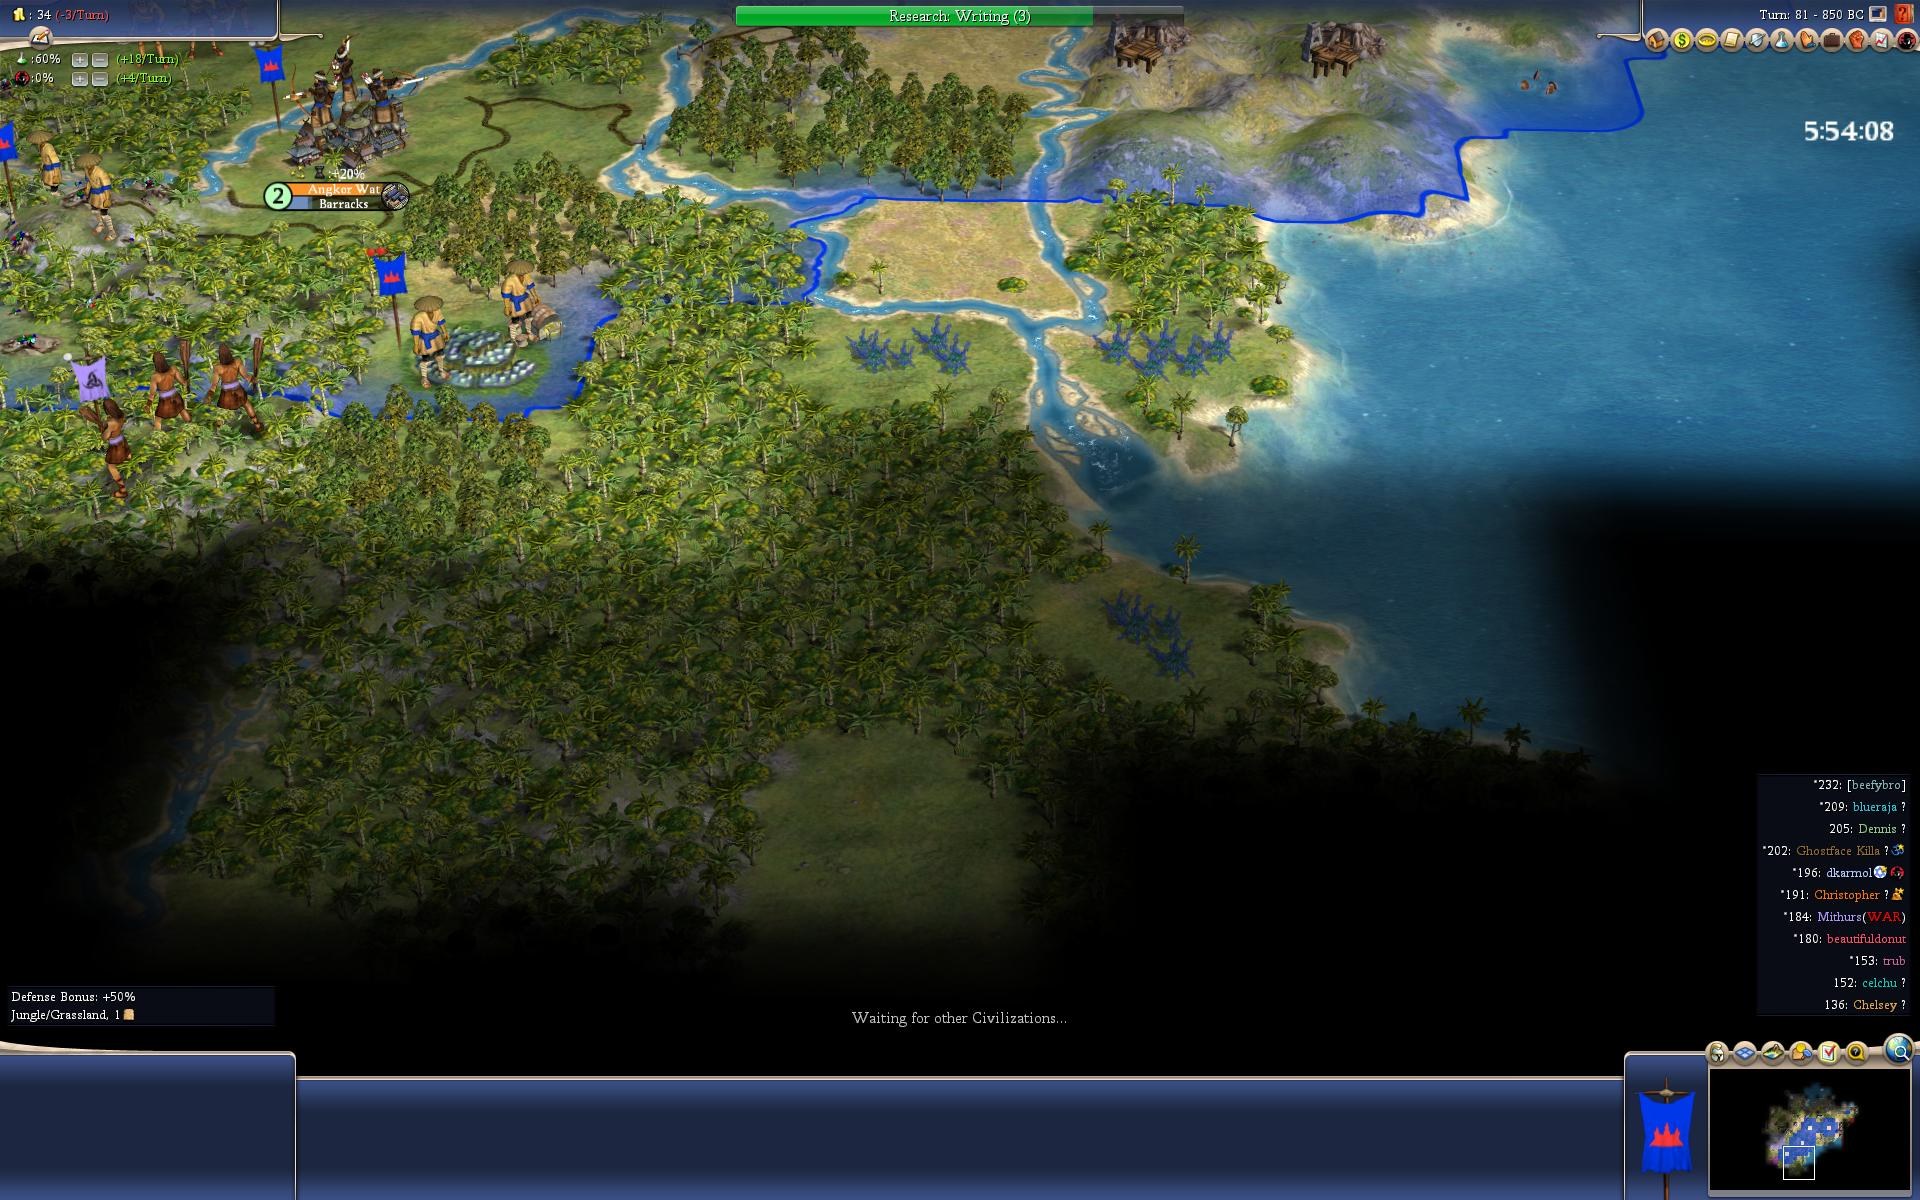
\includegraphics[width=1.0\textwidth]{turn80-3}

The spot near Dave K is probably the most interesting with corn, deer,
and is my only possible iron. Downsides are how far away it is and
it's placement will surely upset Dave K.

The Dye spot is decent, but heavily jungled and without food nodes.

The northern spot is also far away, but picks up lost of happiness resources.

\section*{Turn 90}

I'm paying the price for forgetting to add a no-resettlement clause to
the peace agreement between Drew and I. He immediately realized that
the culture he had established on critical tiles still remained even
though the city is gone, so I'm going to have to give him a free gem
to bribe him not to resettle.. ugh; nothing gets past that weasel.

On to the major issue: city \#5. I initially thought my only option was
to steal the iron city from Dave K, but after a long discussion with
Drew, I decided to be more diplomatic about things. I approached Dave
K with an offer: I'll agree not settle that spot in exchange for him
trading my the extra iron he has in exchange for gems and dye. This is
a pretty good deal; the city is pretty far away and would represent a
big tax on my economy in the near future.

I went ahead and founded city\#5 in the jungle to grab the dye. To my
surprise, the location 1S of the original planned spot is actually
quite good, 4 dye and 1 copper in the BFC. The danger is angering Dave
C and/or Aaron; Aaron seems to not be too offended by the city plant;
I still need to figure out what's going through Dave's head. An offer
of free dye might be in order.

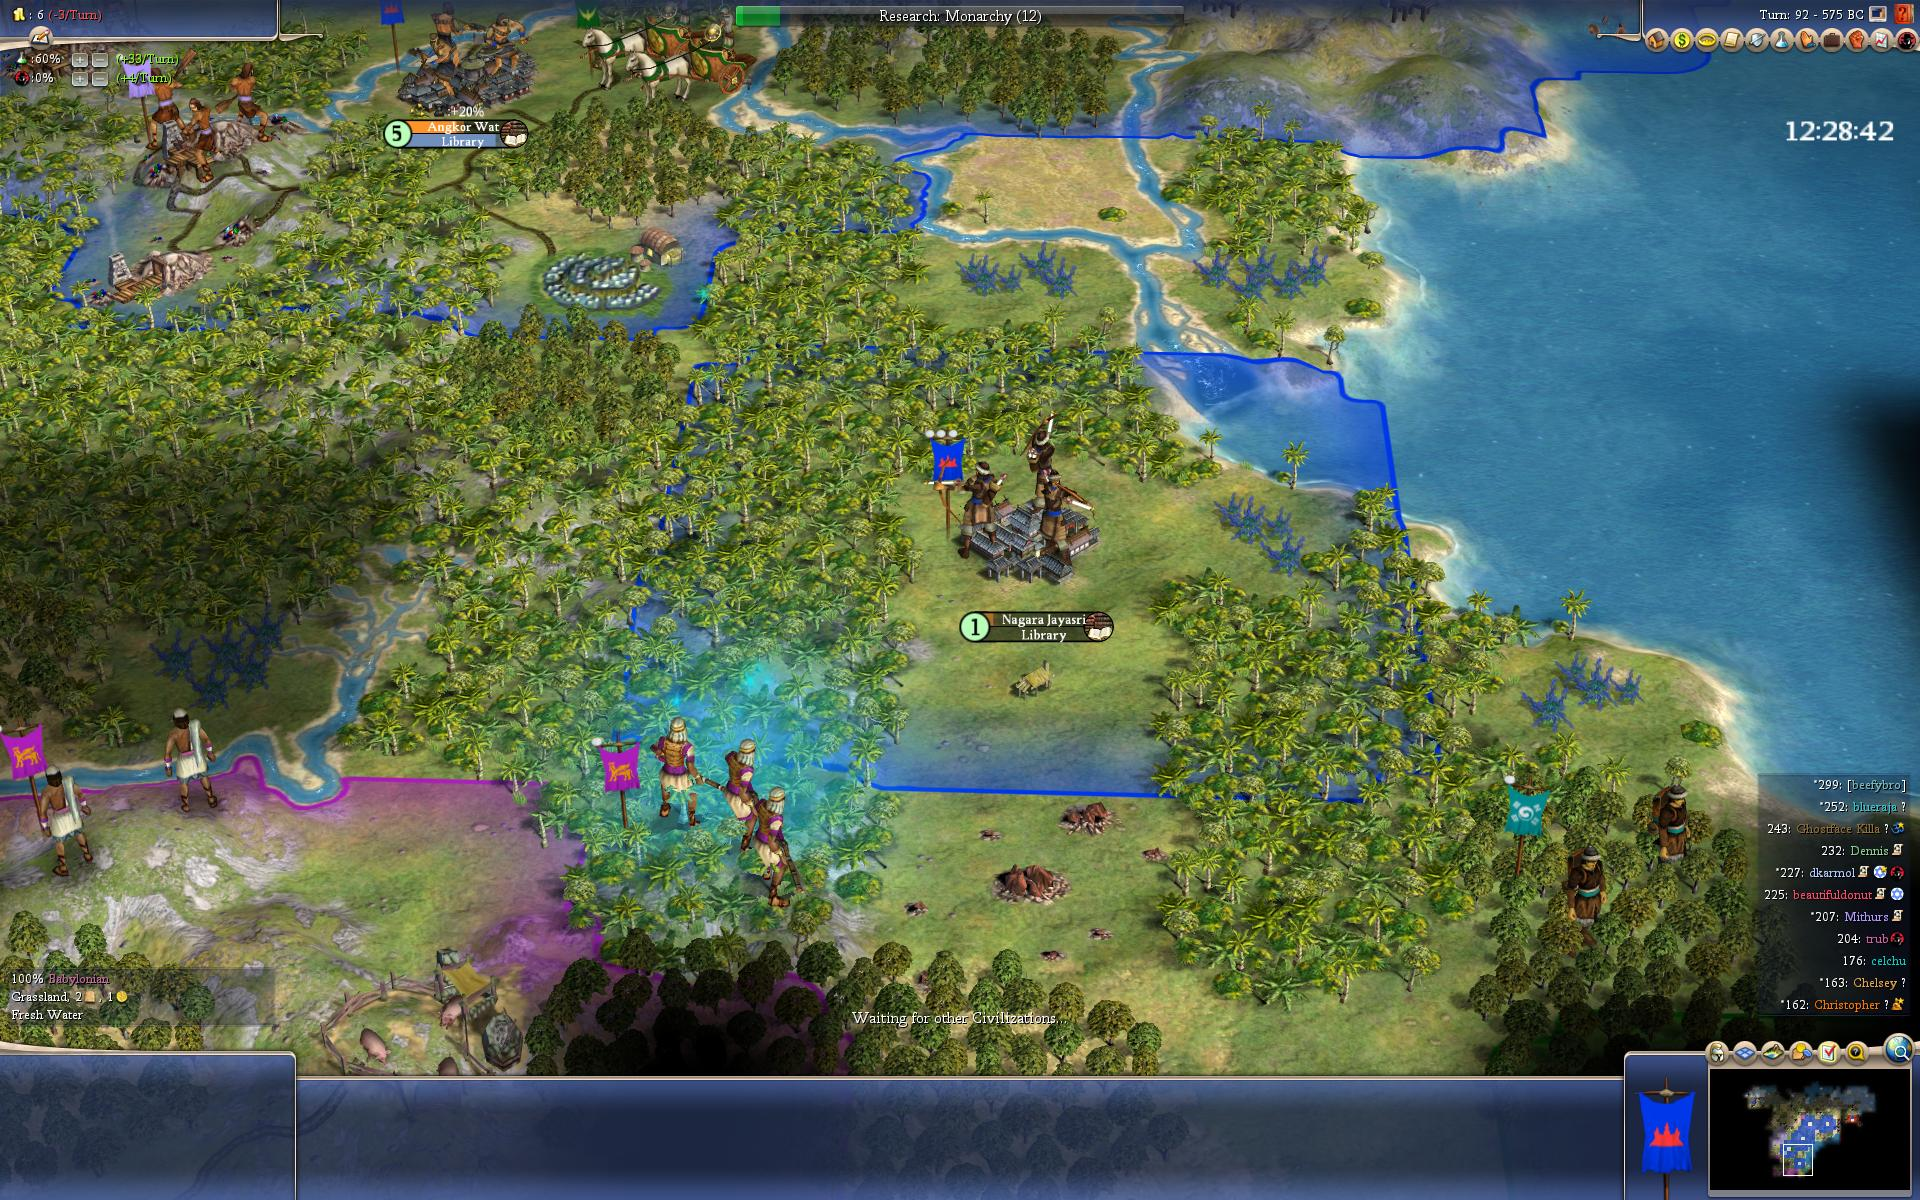
\includegraphics[width=1.0\textwidth]{turn90-1}

City \#6 will go 2N and 1E of the wine, giving me a coastal city that
grabs wine and cow. Drew is going to take everything west of this
spot, which I suppose I can live with.

City \#7 will be a very mediocre city on top of the stone:

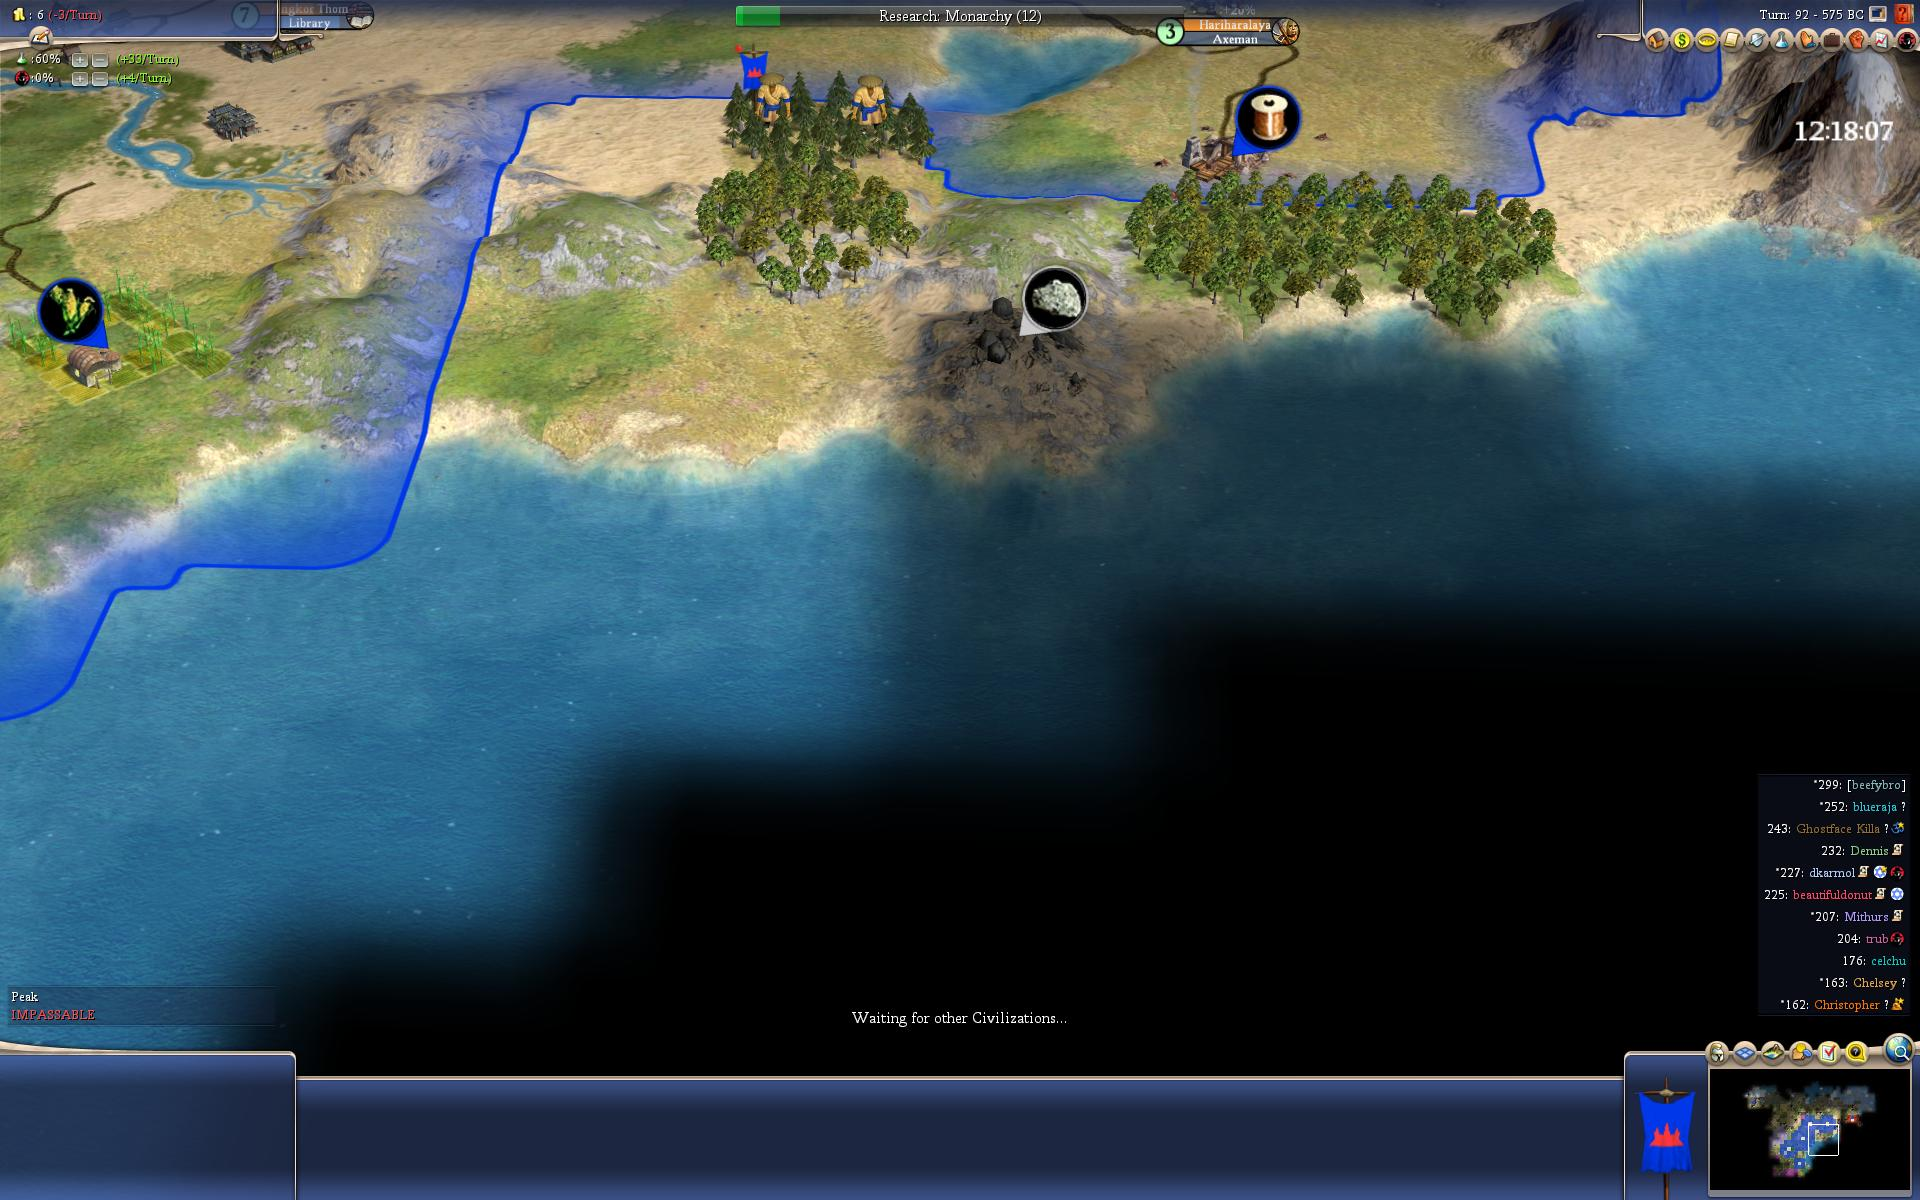
\includegraphics[width=1.0\textwidth]{turn90-2}

With farms on green tiles, using beauracracy to spread irrigation, this will be an OK coastal city.

I'm dominating demographically:

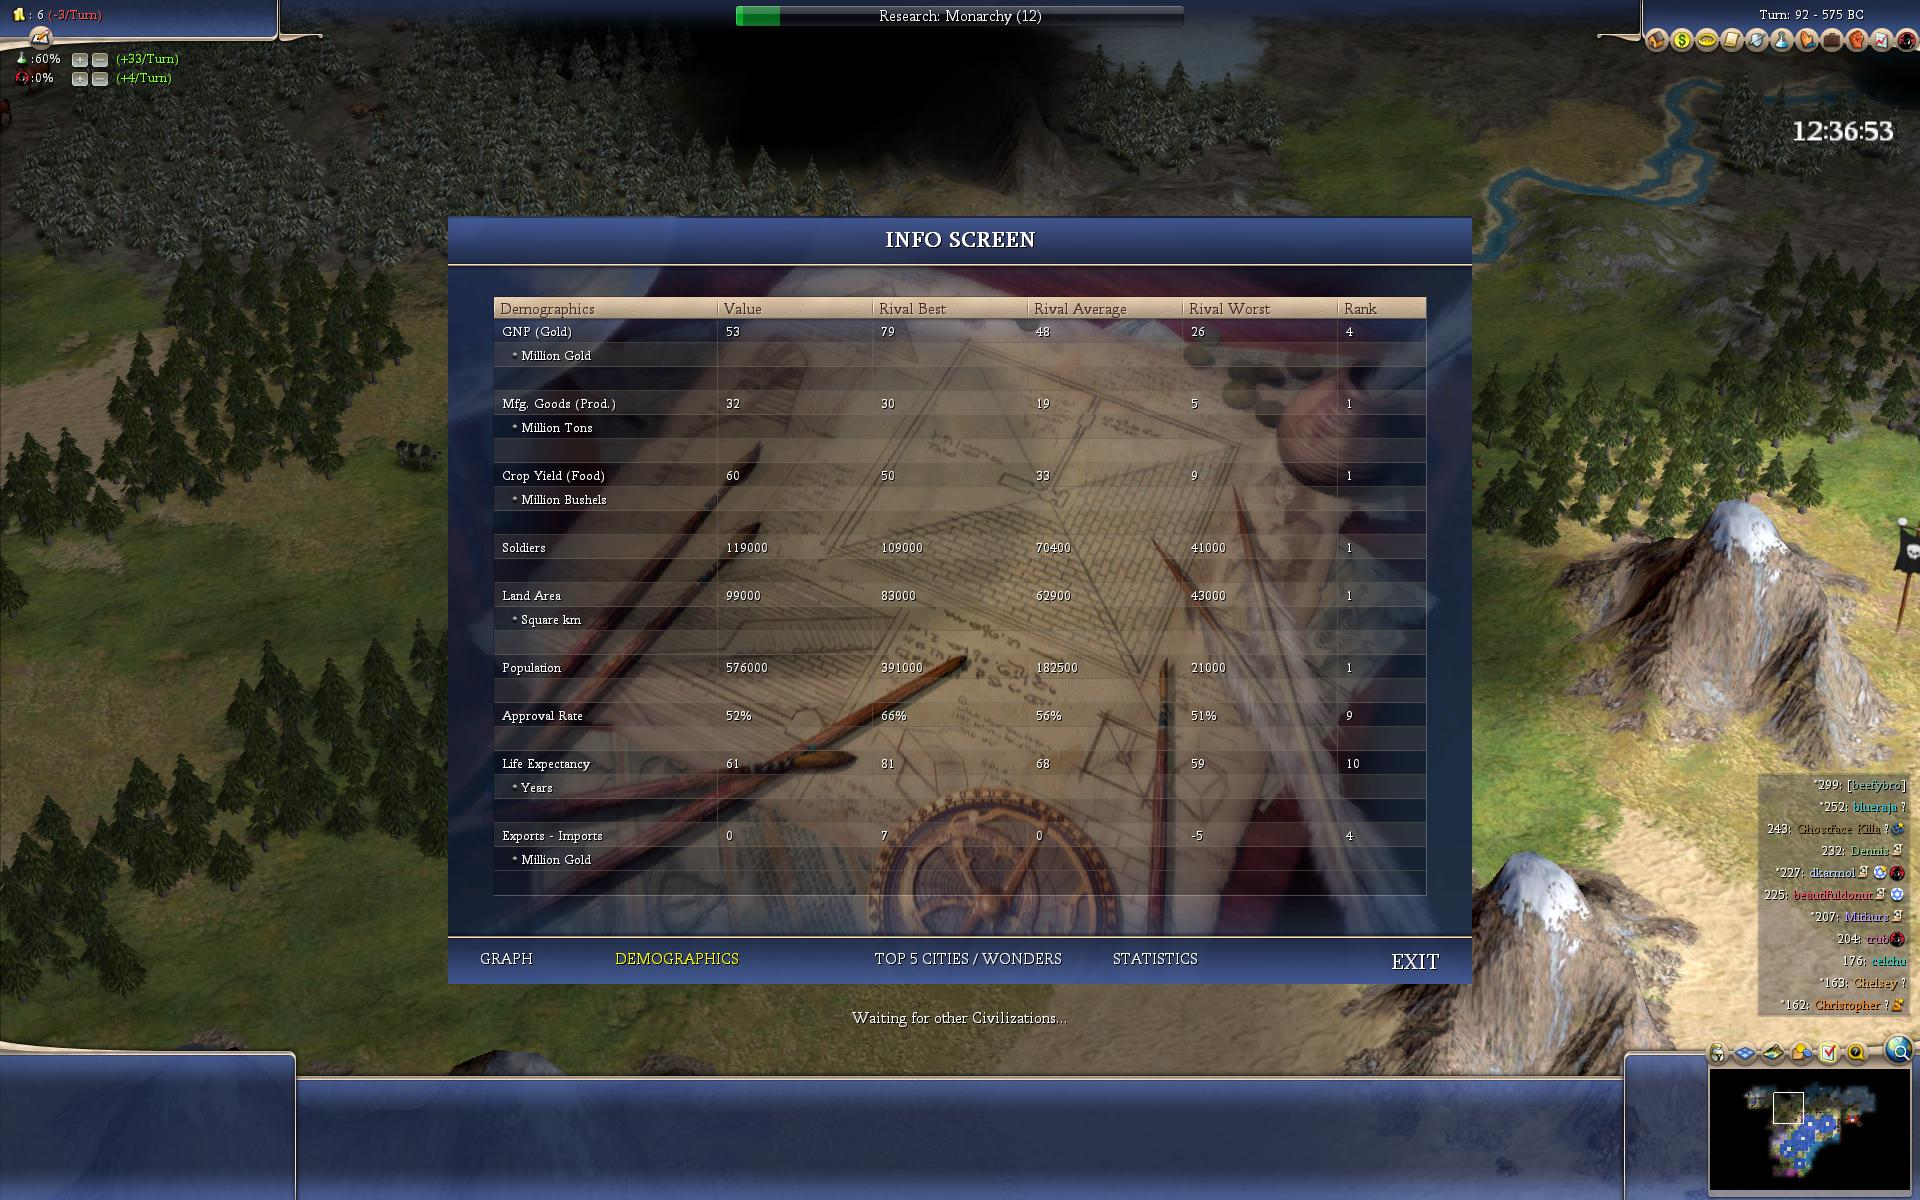
\includegraphics[width=1.0\textwidth]{turn90-3}

and it's starting to show in the score as well; bring on the pile!

After libraries are done, I'll switch over to heavy commerce in all cities except the military pump in order to pick up monarchy fast.

\section*{Turn 103}

Switch to monarchy went well and all cities are now growing again. The
science slider is worryingly low at 40\%; the fact that I'm running 2
scientists in 2 cities is keeping my science rate decent. Hopefully
code of laws and courthouses will fix my bugetary problems.

Demographics show dominance but not runaway:

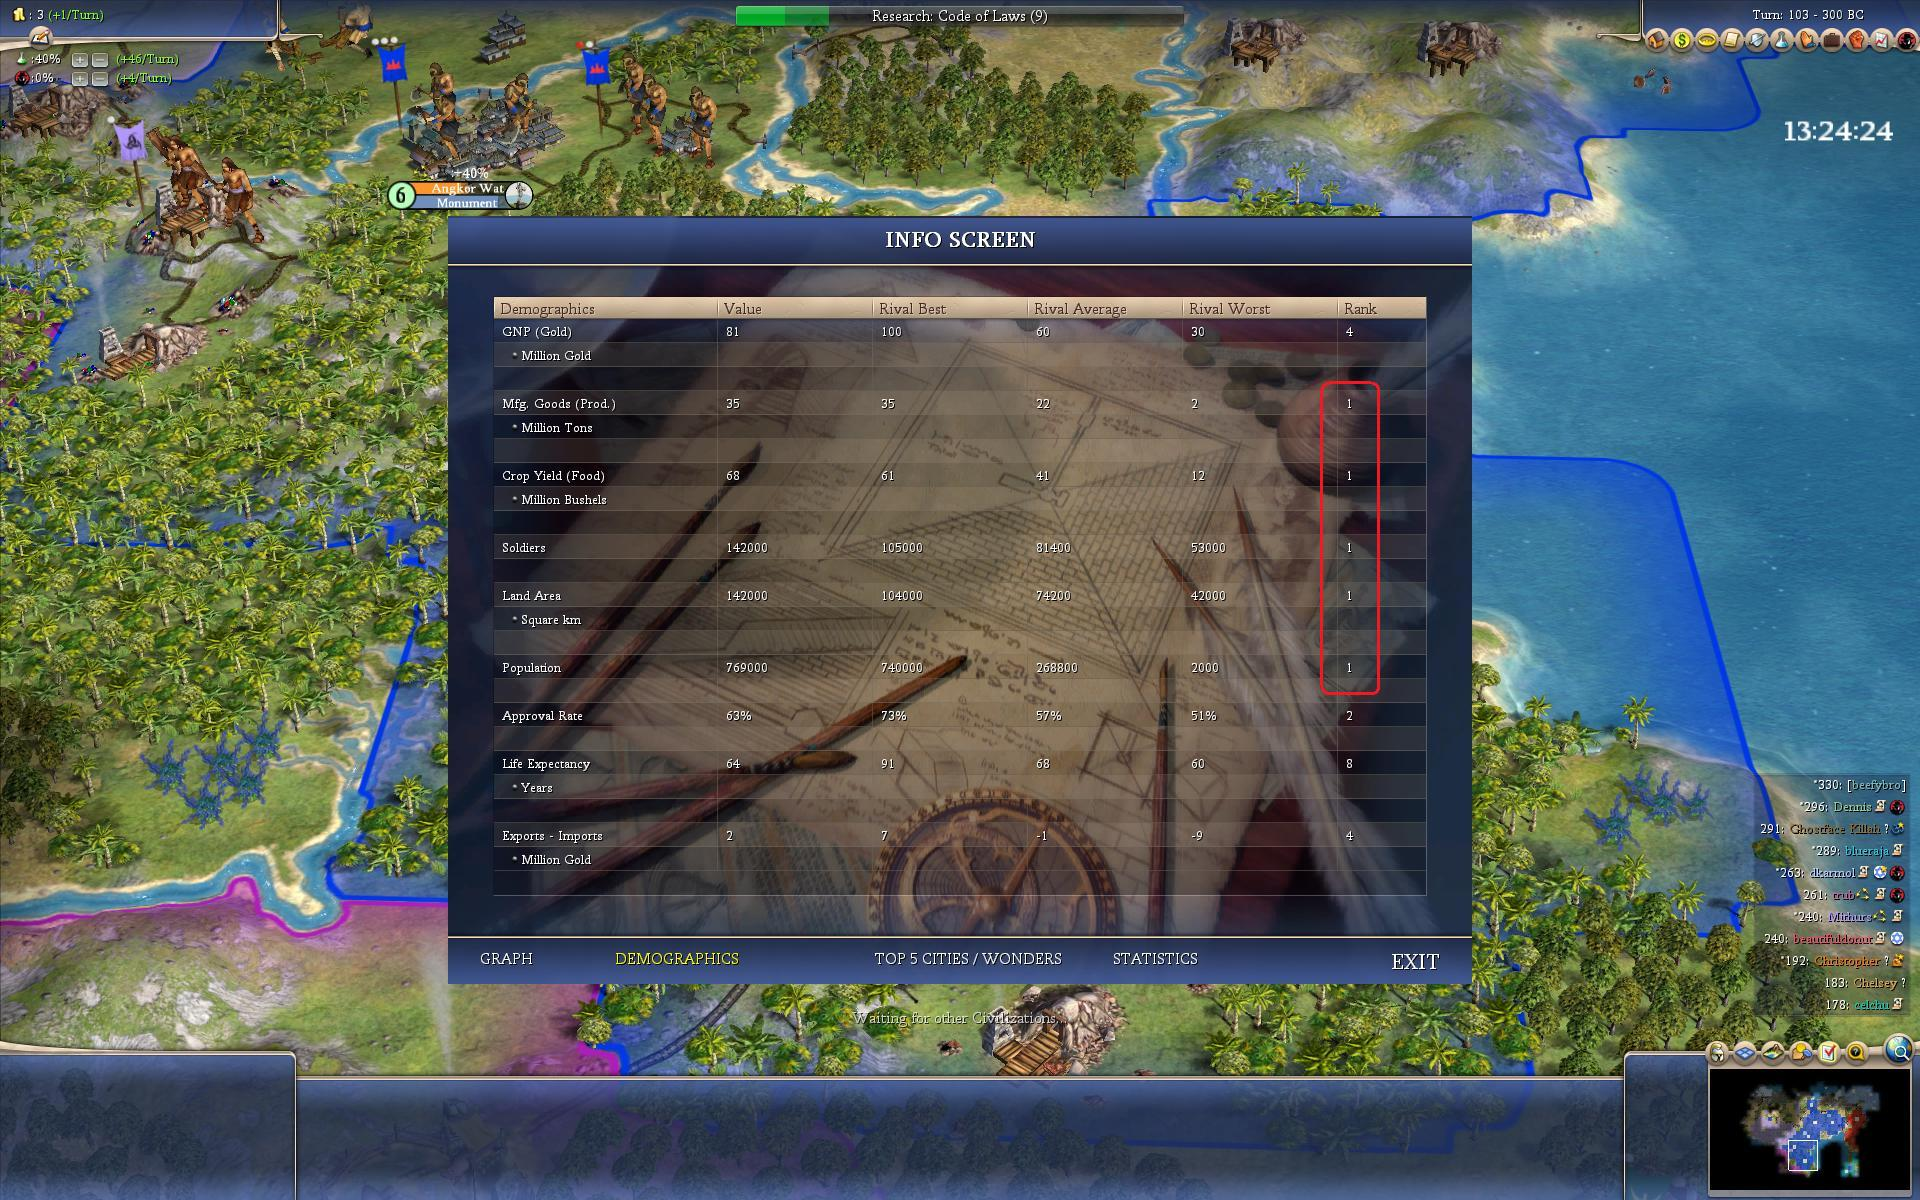
\includegraphics[width=1.0\textwidth]{turn103}

City \#6, described in the earlier post, was founded. Hopefully harbor + trade routes can make this an OK city.

The interesting short-term decisions are all related to the order in
which techs are researched. I'm tempted to beeline civil service for
beauracracy. Other options are to get sailing for better trade routes
or math and calendar to pick up resources.

In the longer-term, I really don't have a good idea of where to go
with my civ. My army is large and is costing me maintenance, but I
don't really have a good target for attacks. Drew continues to settle
all over me but we have a NAP until turn 130. After city \#7, there are
not really any good spots to settle. I'm in a good position with the
land I have, but it's not dominant; I'll need a couple more solid
cities before I can get complacent and unfortunately this means
war. Double the unfortune because Drew is the only logical player to
attack unless I want a very stretched-out empire. I'd rather have him
as an ally, but I don't see how that's going to work. He's managed to
carve out a large plot of land for himself and will be a rival as the
game goes on.

In the meantime, I need to discover the other players for routes and tech bonuses.

Plan: Instead of going too deep for CS, I'm going to go: Fish,
Sailing, Masonry, Math, Currency, Calendar, *then* CS. That should
yield benefits for my economy without stalling my tech for too
long. After that, possible engineering rush for castles, nortre dame,
and trebs?

\section*{Turn 104}

Negotiations with Dave K don't seem to be going anywhere, so I'm just going to take the iron city.

\section*{Turn 109}

Tensions with Karmol are skyrocketting... there has been drama on the
mailing list over server issues that I won't get into here and then
there's this city placement by him:

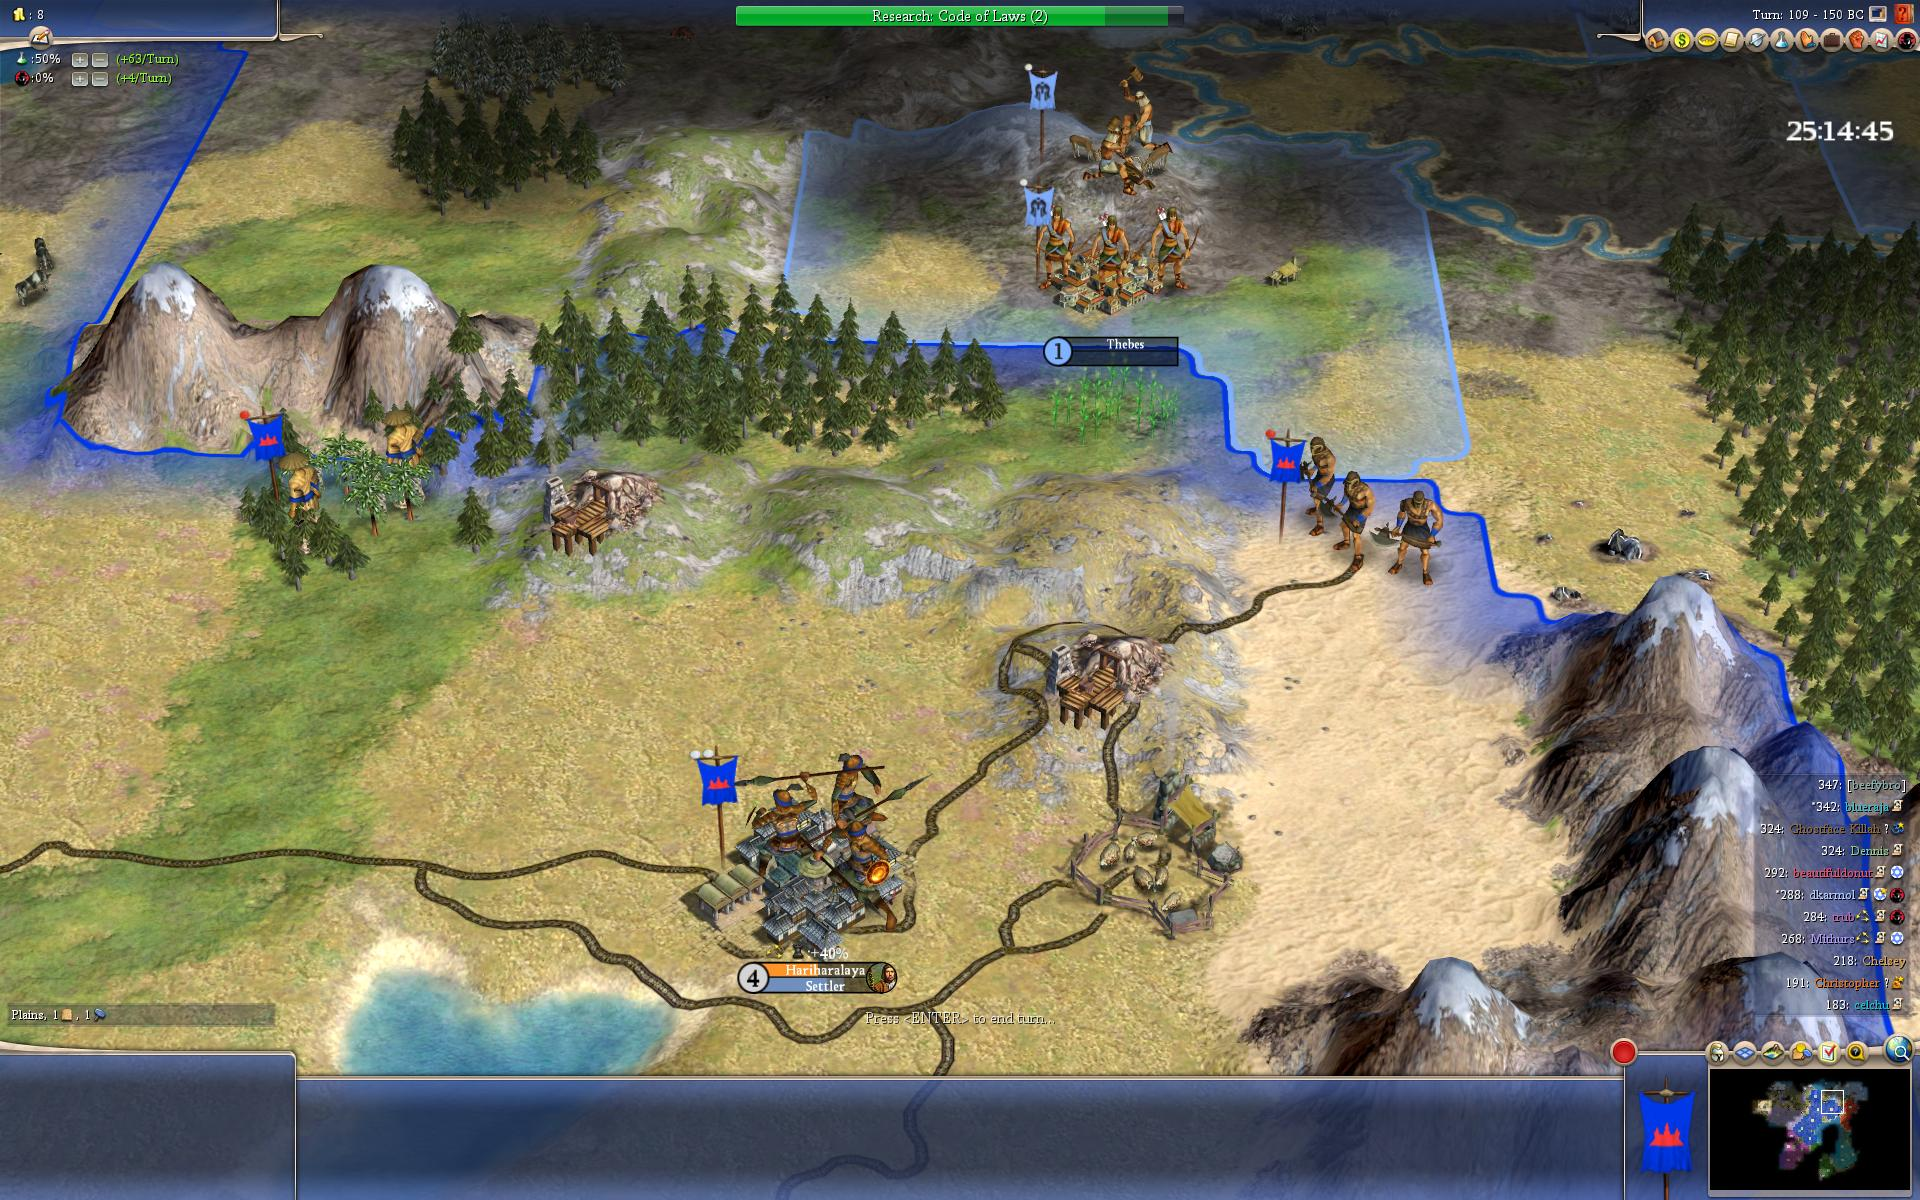
\includegraphics[width=1.0\textwidth]{turn109}

This is a bad city plant for so many reasons that I don't know where
to begin. I think he must have been seduced by the fact that this
would be an epic production city if my borders weren't all over it.

The culture situation simply doesn't add up here for Karmol. My city
to the south is my oldest city (besides my capital of course) and it
has built up a huge amount of culture in this area. Even as creative,
he's probably looking at 30+ turns until he overcomes my borders to
the south; without any buffer between this city and my borders, the
city is virtually indefensible. So what does Karmol do? He puts a
single archer in it even though he can see my axeman 2 tiles away
*boggle*. I guess a super-aggressive plant like this could make sense
if it were backed by a large army and/or the diplomatic situation
between us was good. I can assure you that this isn't the case. I've
made it clear to Karmol that picking up that iron was a high priority
for me and I approached him with a couple of deals that would have
been mutually beneficial; his response is always "I'll get back to
you", which of course never happened. This city placement makes any
deal with him impossible: it prevents me from settling in the area and
it does not pick up an additional iron (that he could trade to me) in
a reasonable amount of time. This makes the decision for me pretty
easy: WARRRR! If the archer gets lucky and defeats the axeman, it will
surely fall to the spearman.

\section*{Turn 111}

Karmol's city was captured easily; however the diplomatic picture is
muddy. Karmol claims that he founded the city at that spot due to
misinformation from me regarding the location of the iron. It's
certainly possible, however you'd think he would double-check before
making the plant that he did. Anyway, like I said to Karm, it was all
a moot point after the city was founded. The position of the city
meant no possibility of iron for a long time and that's not
acceptable, so down it went. Now comes the hard part of figuring out
what to do with Karmol diplomatically. I'm kind of tempted to just
finish him off; it seems unlikely that we can work together after
everything that's happened.

Other factors:
\begin{itemize}
\item I have a big army and nothing to use it on... until now
\item I need to expand in some direction to keep up with Pat. Karmol's direction is as good as any as he is fairly weak.
\item I was not keen on being dependent on him for iron
\end{itemize}

In other news: Drew and I have reset the countdown on our NAP, so it's
back to 50/100. I need to remember to keep this deal quiet. He will
also start giving spices for gems.

\section*{Turn 113}

The great scientist/academy rush worked like a charm. My economy has
gone from parity with the other top players to dominant:

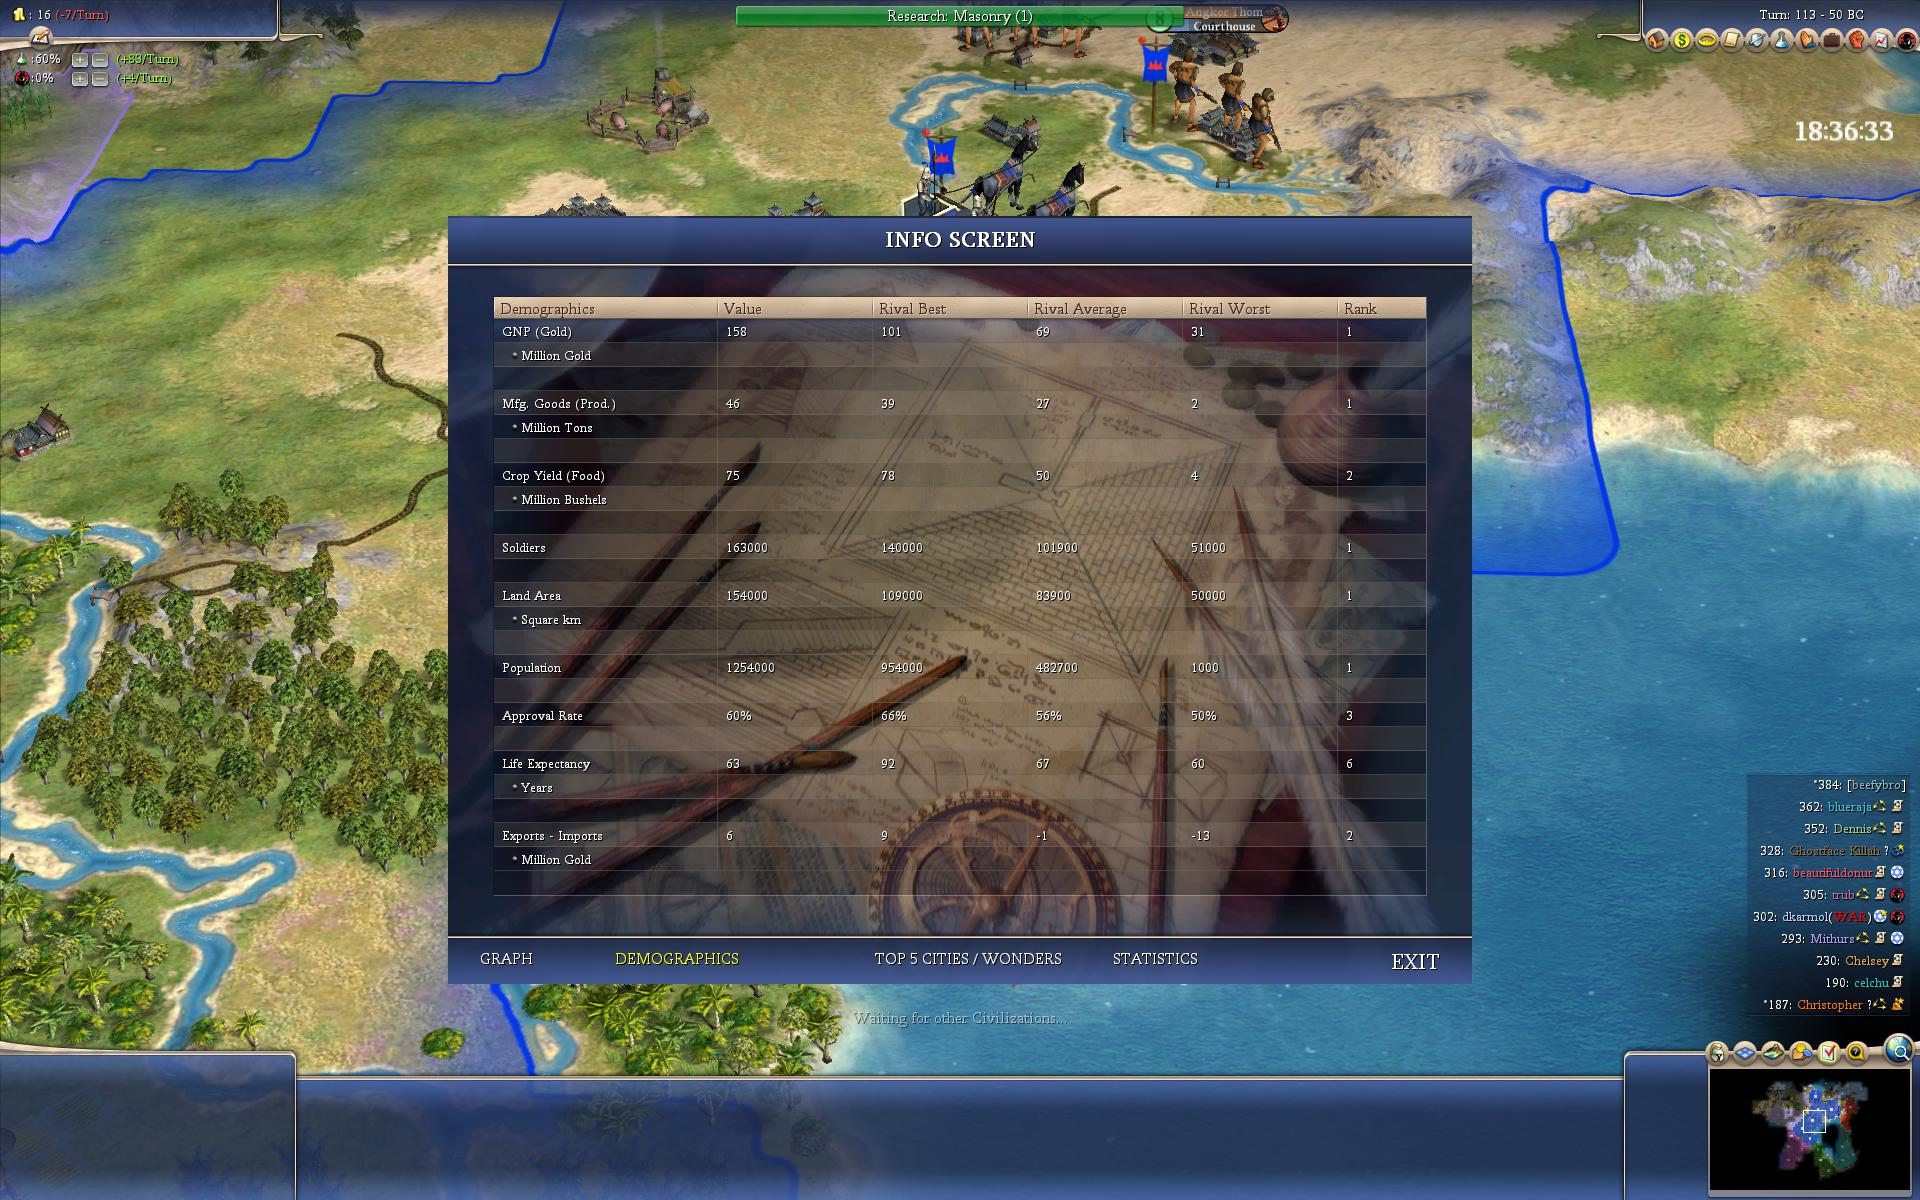
\includegraphics[width=1.0\textwidth]{turn113}

I will try make peace with Karmol; the settler to claim the iron is 1
tile away. If he signs the peace treaty, there will be nothing he can
do about it for 10 turns.

\section*{Turn 116}

The stealing of the iron city is complete; Karmol signed the peace treaty and I plopped the city:

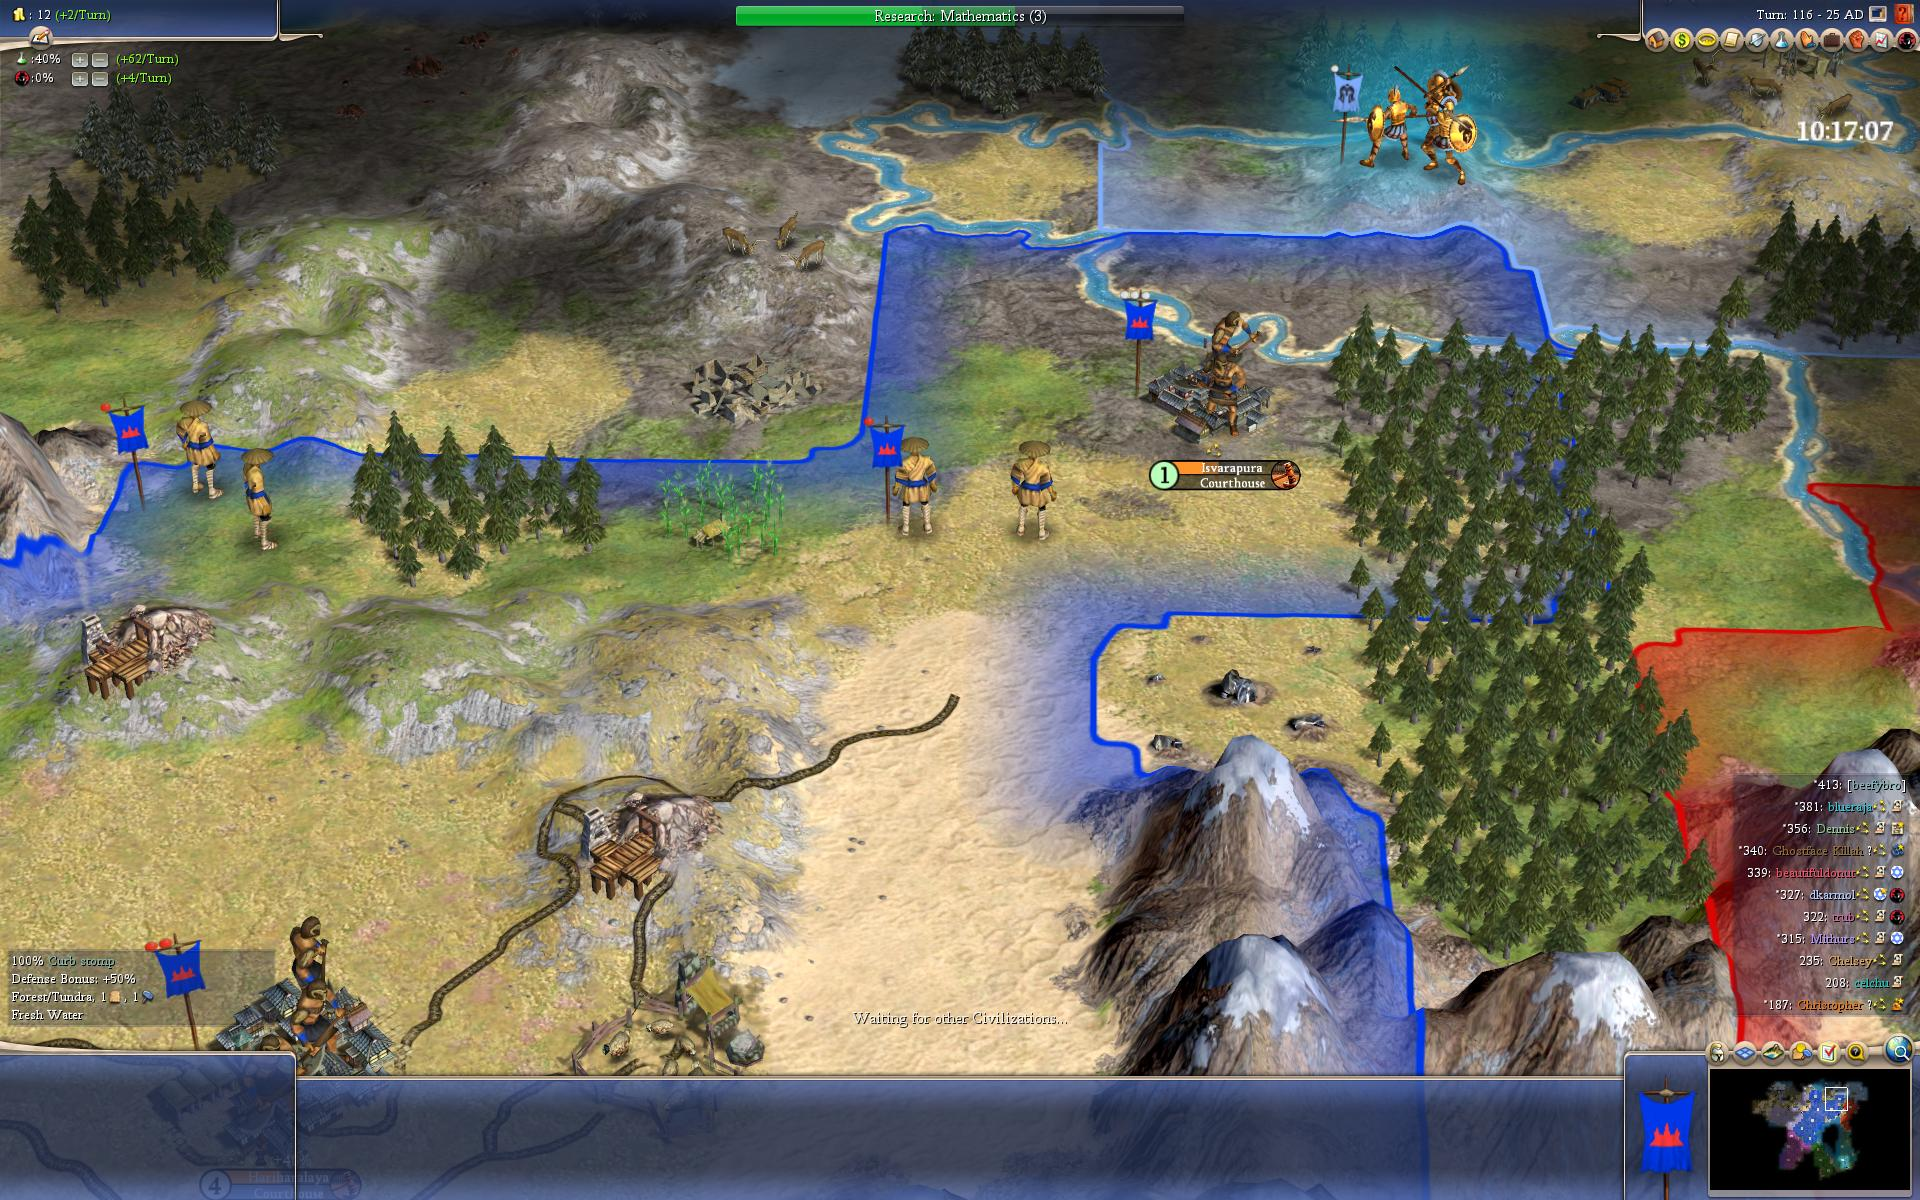
\includegraphics[width=1.0\textwidth]{turn116}

Karmol is going to be extra pissed, so I'm moving 5 units in to defend
the city. I have had to lower my tech rate down to 40\% to support all
the cities, so my economy has cooled off a bit, but is still \#1
(barely). In any event, I think this city could become a good GPP farm
one day.

\section*{Turn 124}

Other players are popping wonders and I'm beginning to lose my
advantage; the most worrisome is Pat's completion of GL, propelling
him to the \#1 score.

I have shifted my focus from a total emphasis on research to a more
balanced approach and I'm no longer running any science
specialists. My happy cap has increased considerably with new
resources coming online and monarchy spam, so I'm more
growth/production oriented for now with cities needing to grow and
make courthouses and barays. This shift has weakened my dominant GNP
position:

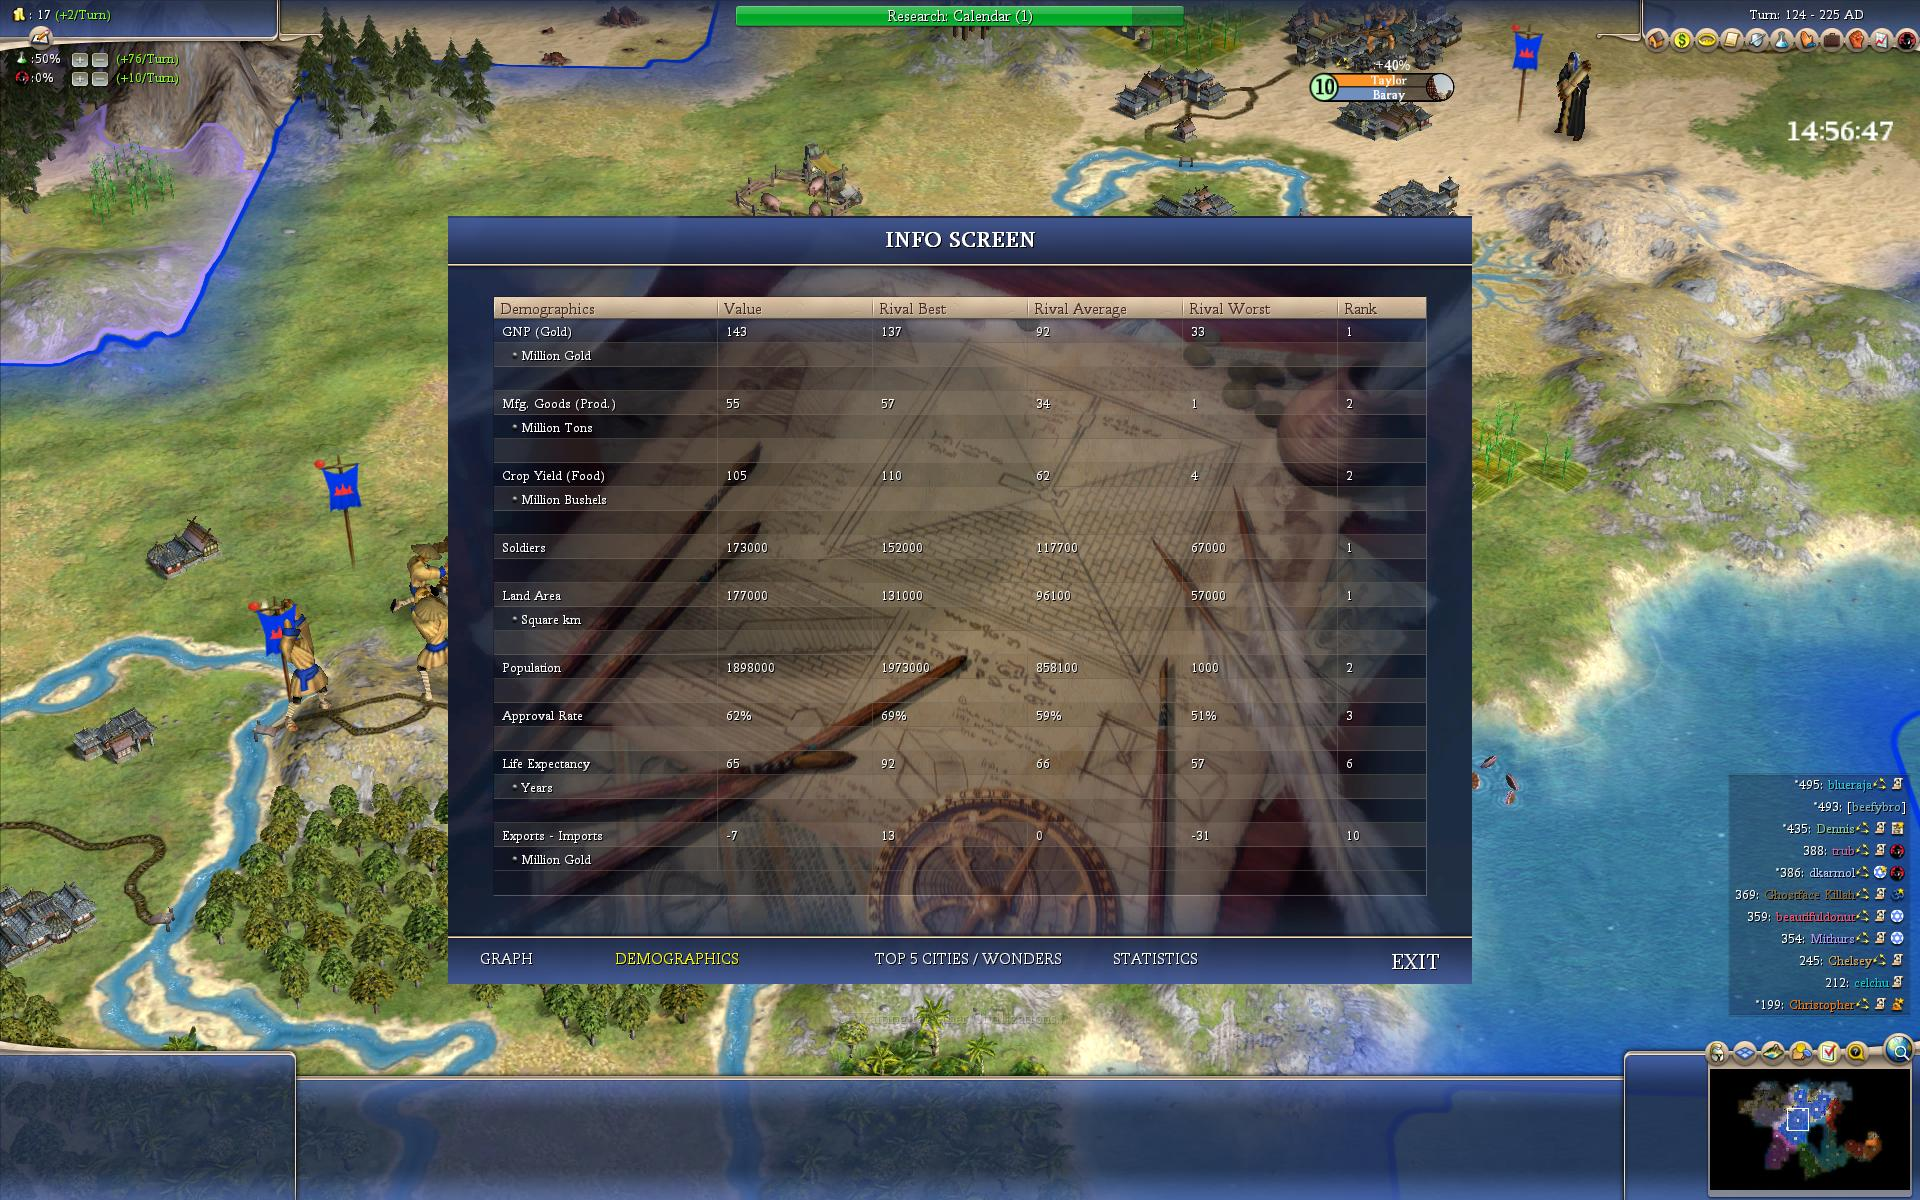
\includegraphics[width=1.0\textwidth]{turn124}

My production feels weak and I'm falling behind. Judaism needs to be
spread quickly to all cities and the switch to OR made; also, metal
casting needs higher priority so I can start getting forges up. With
my recent thinking, the current tech order is: Metal Casting,
Polytheism, Monotheism, Civil Service, Currency, Machinery,
Construction, Engineering

After Machinery is complete, I will start pumping maces. After
engineering, pump trebs. Once I have a large army, I will try to take
DaveK's capital.

\section*{Turn 126}

DaveC's power is skyrocketing and this needs to be investigated. I
should be able to afford to send one chariot that was providing
happiness to the capital down to investigate. Hopefully, if he is
preparing an army for some kind of attack, I can observe it in his
territory and therefore give myself some warning.

\section*{Turn 136}

Pat and I continue to vy for \#1 with the top player switching nearly
every turn. Demographically things are headed in the wrong direction
fast with me conceiding the lead in all of the most important
categories:

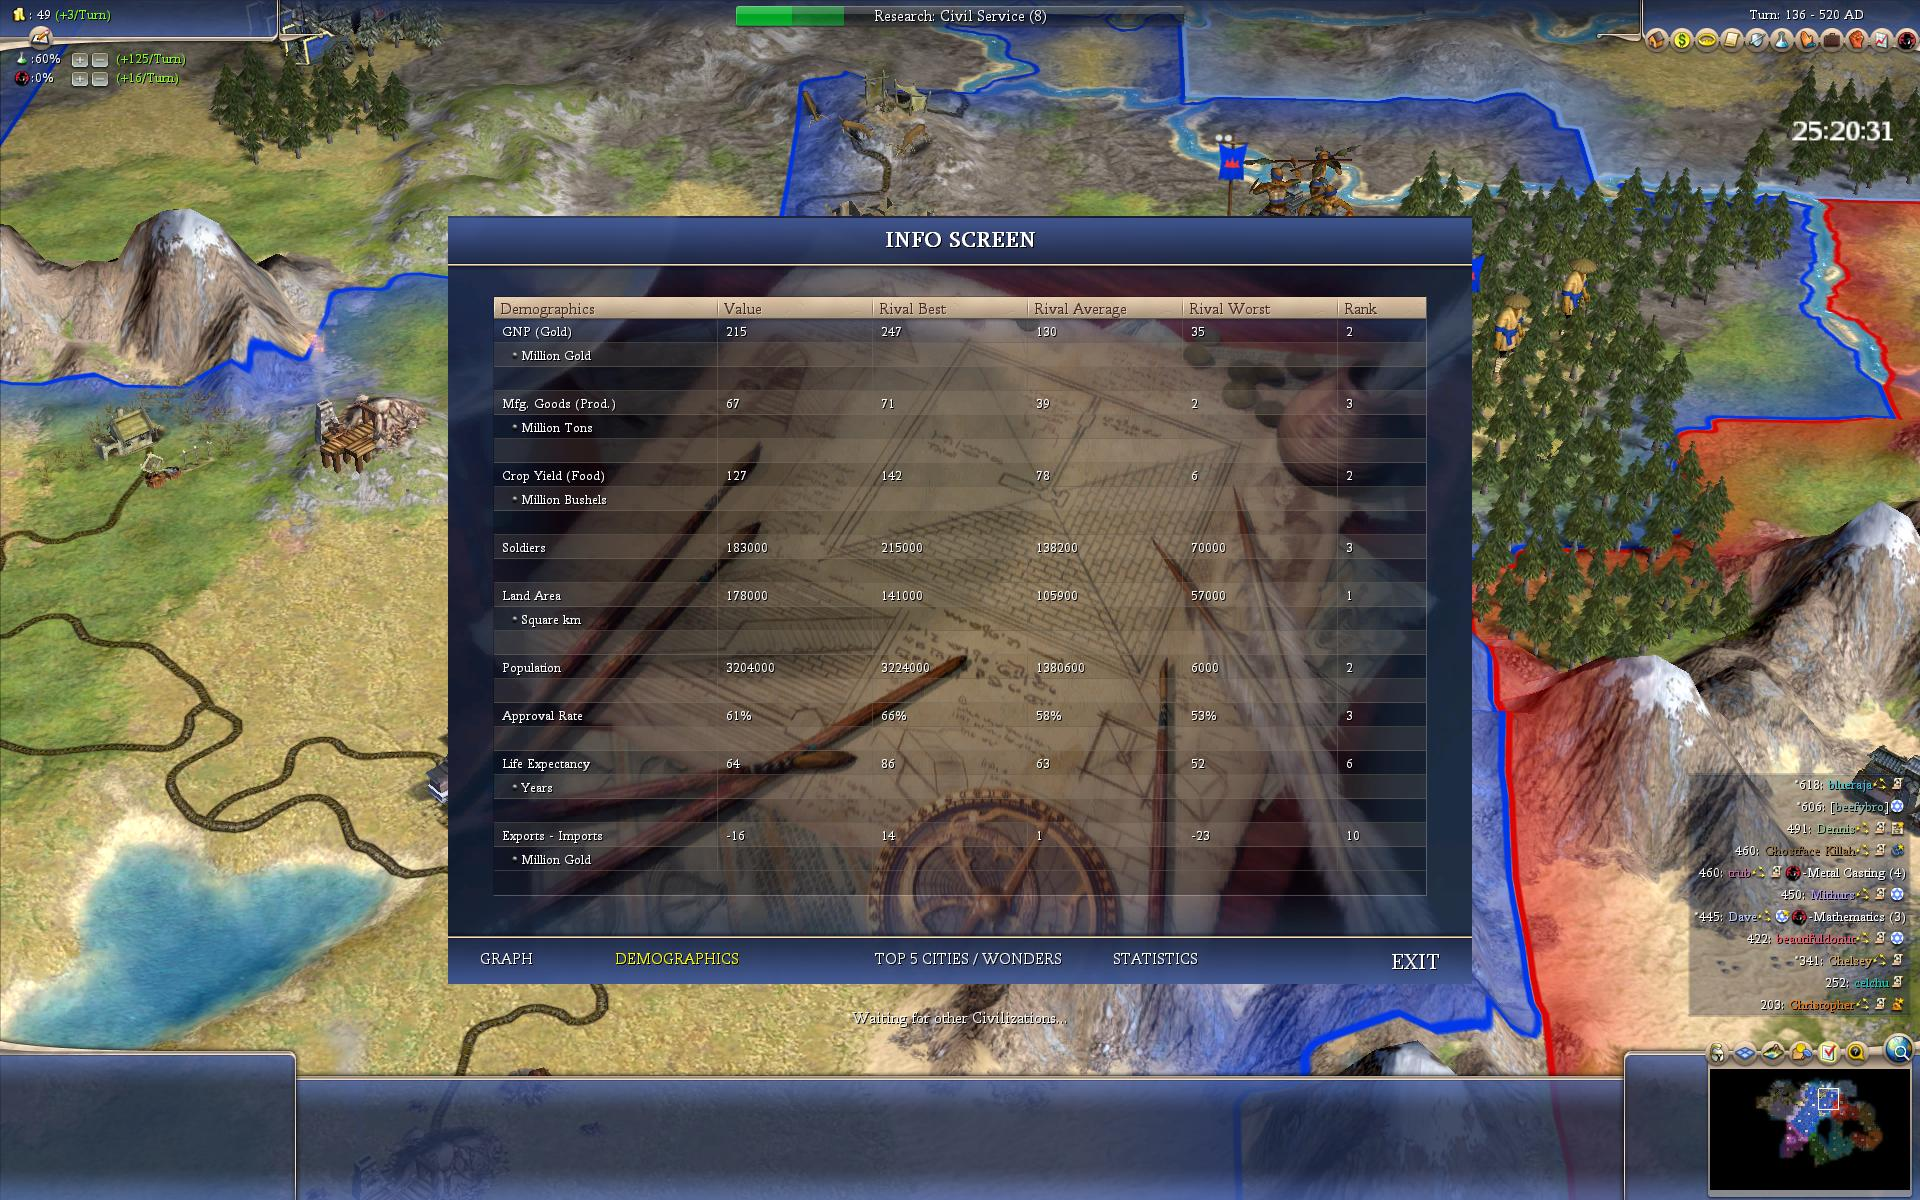
\includegraphics[width=1.0\textwidth]{turn136}

A barb city has spawned in an interesting spot just north of the iron
city I stole from Dave. It looks like Dave is sending over a couple
phalanxs (axemen) and I've sent over 3 axemen and a chariot. Ideally,
Dave sacrafices his units, damaging the archers, and I take the city;
pesimally, I do all the heavy fighting and he gets the city. I have
more units there so this should play out in my favor, but extreme
caution needs to be taken here. There are some interesting double-turn
possibilities as well.

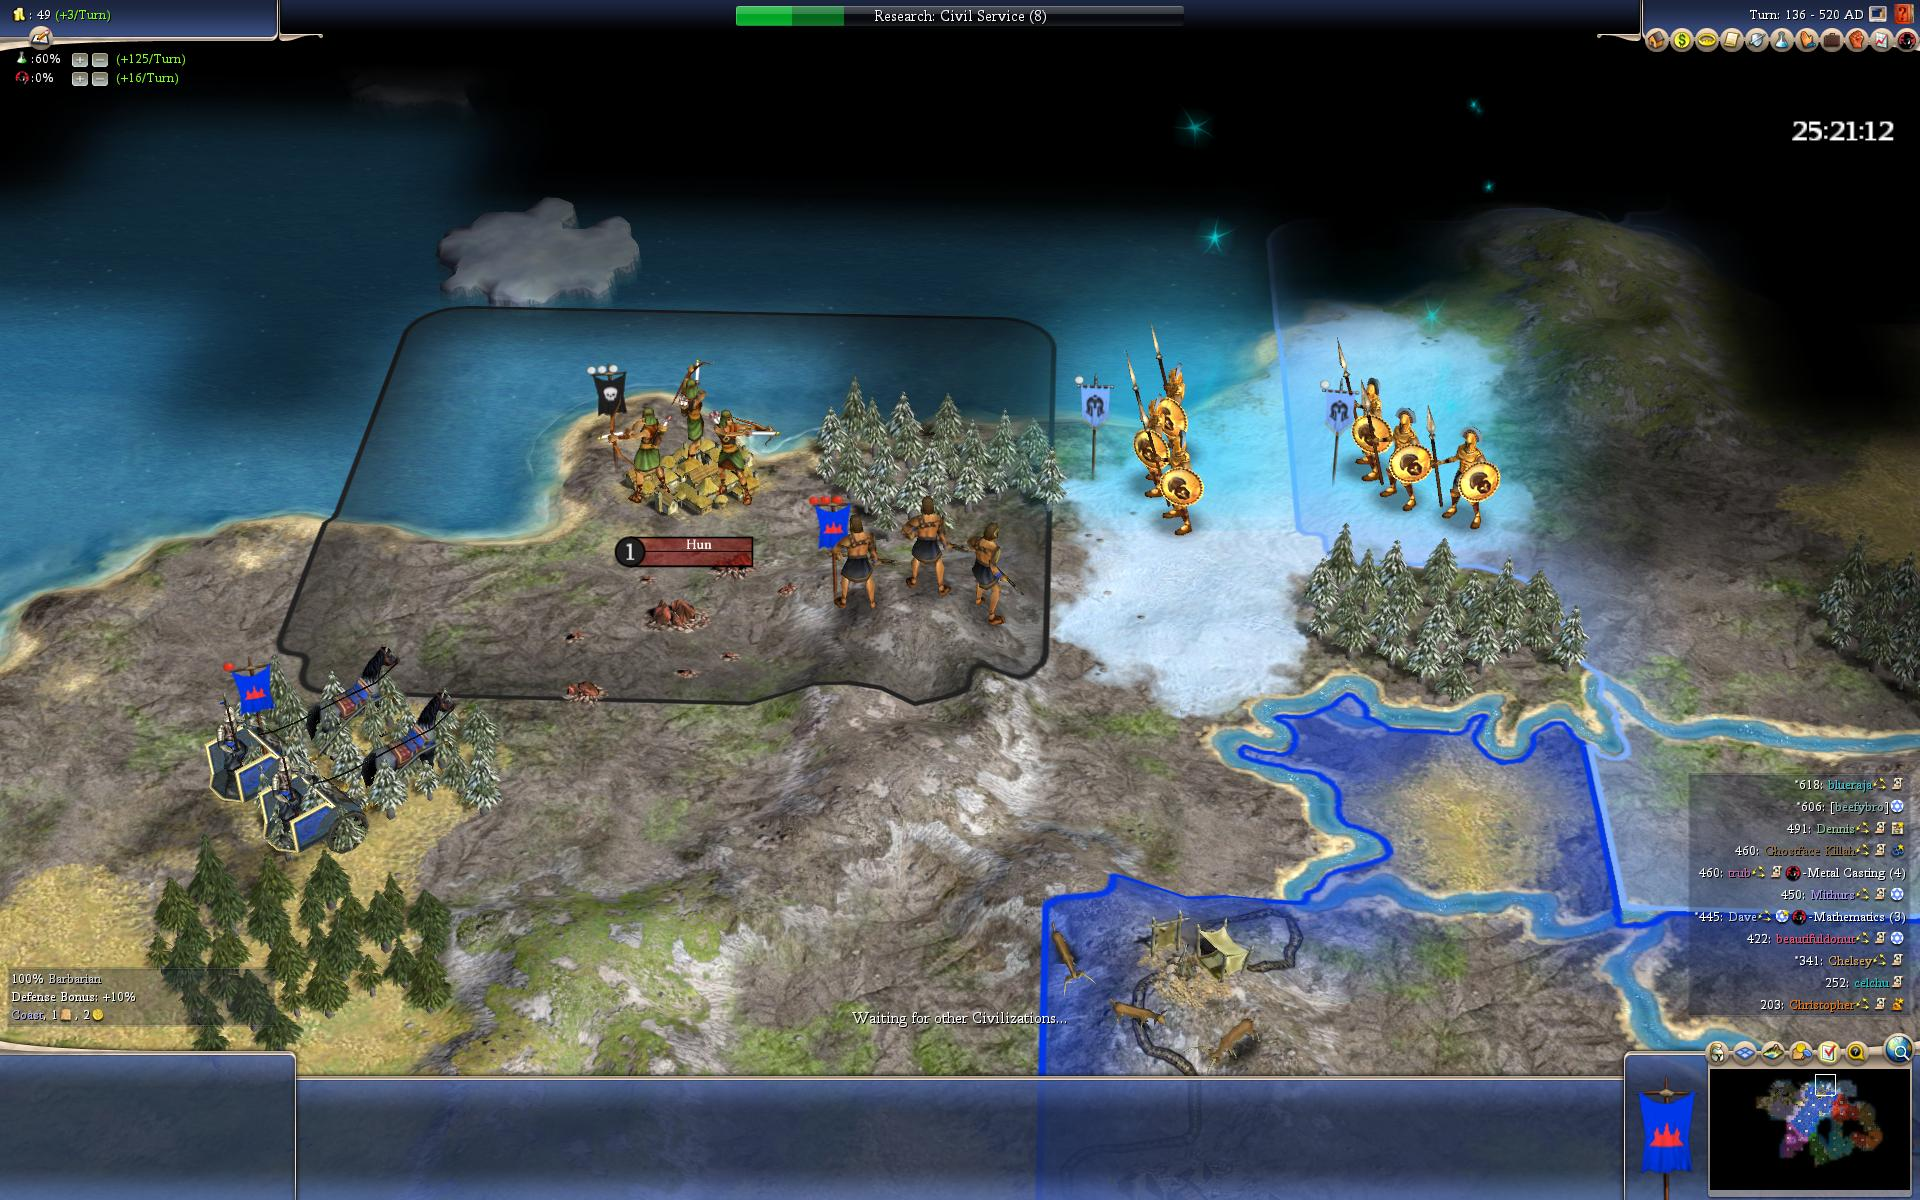
\includegraphics[width=1.0\textwidth]{turn136-2}

Another choice is what tech to get after CS. Currency for economic
growth or machinery to begin the transition to military. I think it's
pretty safe to say, with the demographics going the way they are, I'll
need to take over DaveK in order to have a chance at this.

\section*{Turn 140}

Things are finally getting interesting. I've agreed to participate in
a triple-team pile on Aaron with DaveCop and Pat. In exchange for my
help and free dye, Dave is going to agree to a 100-turn NAP and give
me rights to Aaron's northern-most city. This is a great deal for me
as it ensure a long peace to my south so I can hit Karmol with
everything. Cop also wants a jewish missionary.

With war starting to break out, machinery is definitely the next tech after CS.

\section*{Turn 144}

Aaron's northern city has 2 longbowmen, one of which has city-defense
level 2, so I won't be taking the city without trebs. I have been
pillaging the city's improvements (27g collected so far), but he
hasn't done a very good job of improving the surrounding terrain so I
will run out of things to pillage soon. The interesting issue is
whether to go south and start pillaging the capital's towns. DaveCop
has requested that I not do this... I'm going to wait for a few turns
to see if he really has any chance to take the capital.

The switch to beaurocracy and organized religion is complete and the demographic effect is obvious:

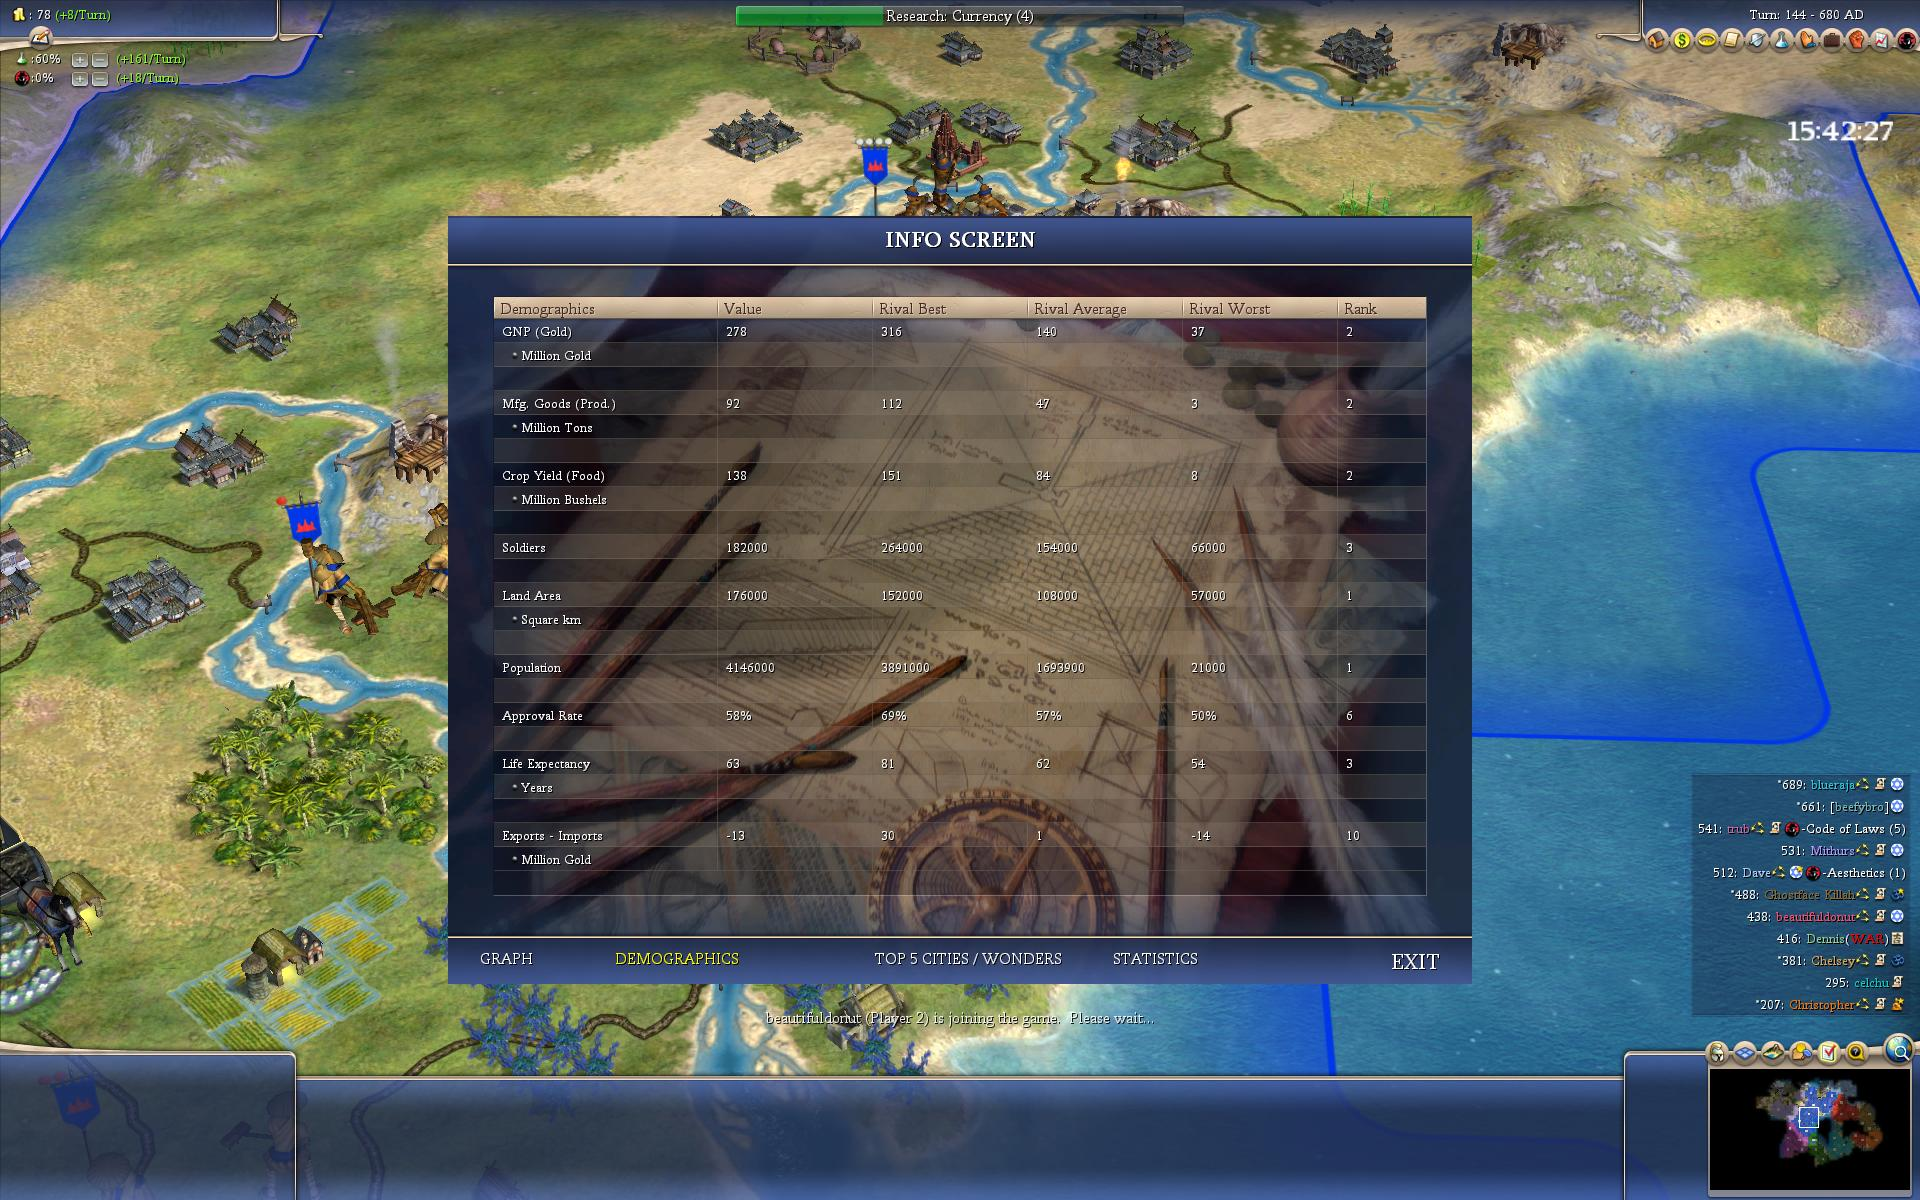
\includegraphics[width=1.0\textwidth]{turn144}

Pat is still ahead in GNP and MFG due to his golden age; once that
wears off, I'll have a better idea where I stand. It still looks as
though my current land will not be enough...

\section*{Turn 148}

Lots of interesting developments.

1) With the discovery of currency, forges, bureaocracy, organized
religion, etc, I am now nearly at parity with Pat in GNP and MFG
despite him being in a golden age. With some skillful peaceful
teching, it is possible that I could pull away without having to go to
war. I'll have to see exactly where Pat is at when his golden age
ends. With long NAPs with most neighbors, I could switch to caste
system and go heavy scientists in all cities when there wasn't any
useful infrastructure to create. This could get me to liberalism
first...

2) There are several excellent pillage tiles near my force that's
attacking Aaron. If I can convince DaveCop that he cannot take the
capital (5 double-promo'd longbows on a hill), then perhaps he will
let me pillage those tiles. The income from pillaging would allow me
to run deficit research and could ensure that I get liberalism.

3) DaveKarm is beelining theology and is clearly going for the
apostolic palace. This will make it very difficult to attack he or any
other jewish civilization. I could still maybe beeline his capital
before he called a "stop the war" vote or I could convince some jewish
players to vote against it. In any event, it makes my previous plans
to attack him less appealing.

4) Lynda appears to be interested in dye; perhaps I can get some GPT from her.

\section*{Turn 151}

Pats golden age is finally over and it looks like we are roughly at
parity; he is slightly ahead in GNP and I have an edge in MFG. With
him being financial and having the great library, this is still not a
great position so I still need to go to war. I think I can convince
Lynda, Drew, and DaveCop to vote against a "stop the war" resolution
which opens the door for war against DaveKarm again. The attacking
force will be trebs, maces, and knights.

The war between Brad and Lynda appears to be legit, so there's no reason to pile Lynda.

\section*{Turn 160}

The game is back up after a long downtime over holiday break. Recent
developments have reinforced my belief that I'm not quite in a winning
position with my current land; particularly worrisome is Pat's huge
lead in food collection (I now have enough espionage points on Pat to
see his demographics):

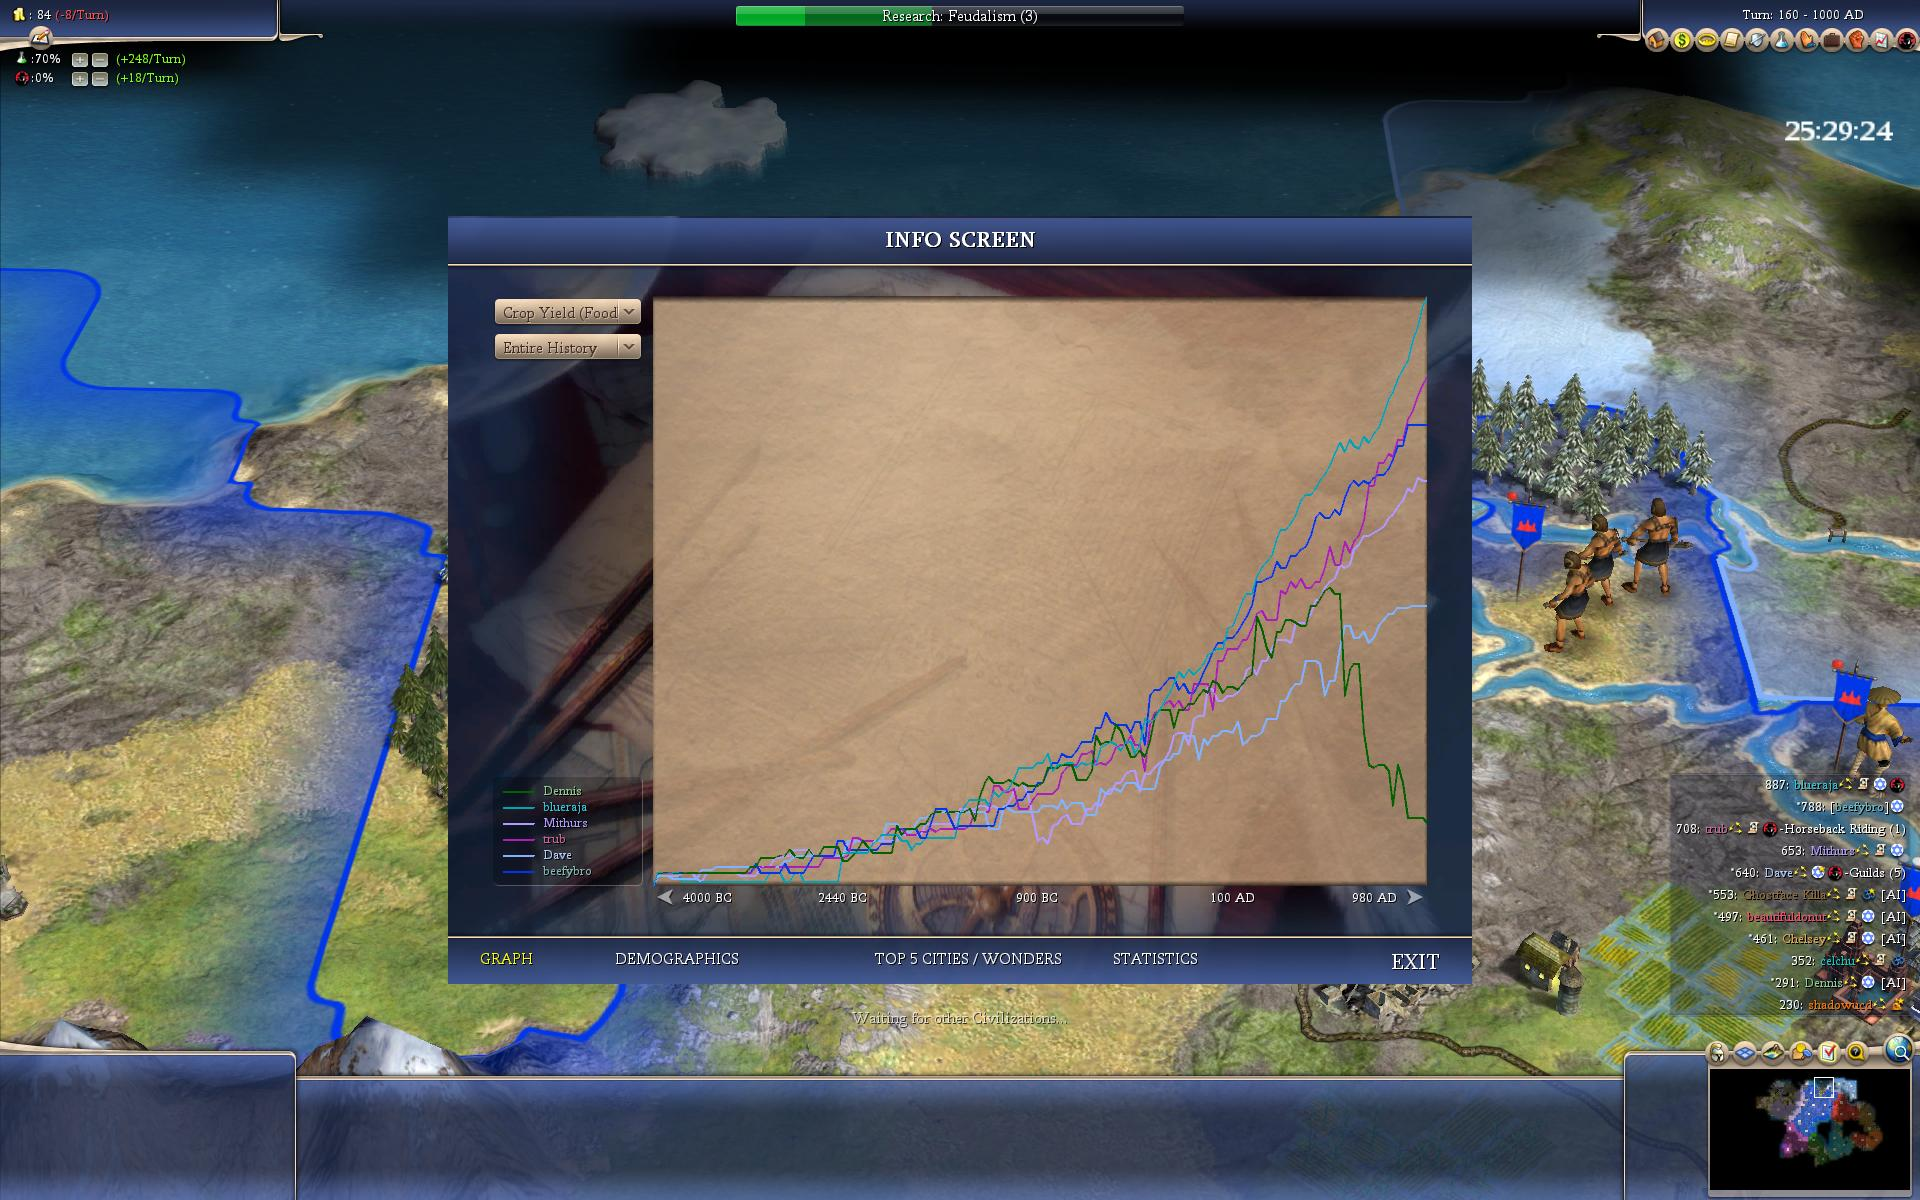
\includegraphics[width=1.0\textwidth]{turn160-1}

My economy is almost as good as his and my MFG is still slighlty above:

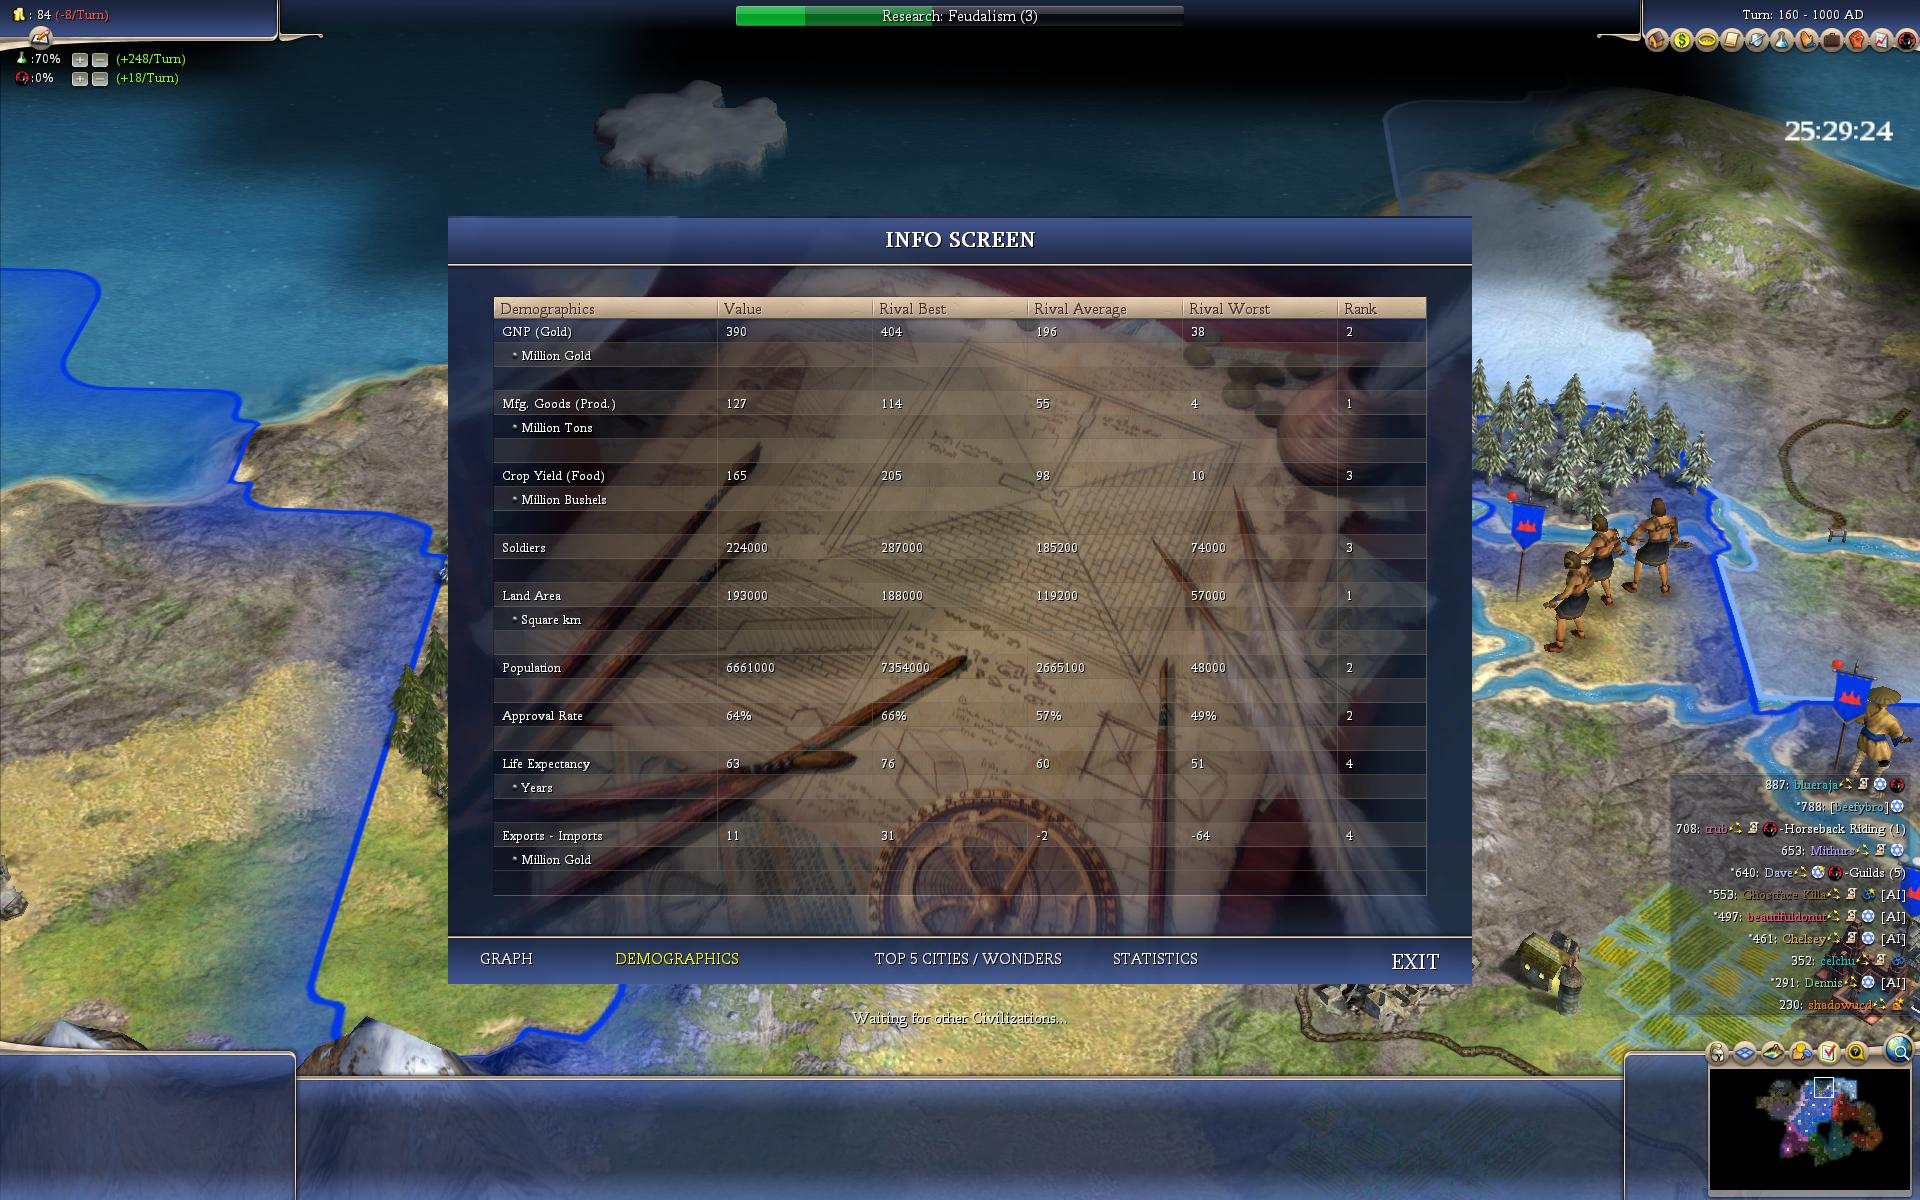
\includegraphics[width=1.0\textwidth]{turn160-2}

... but with such a huge food advantage, his civ will surely outgrow
mine over time, which is basically what I've been seeing over the last
50 turns or so. One comforting thing is that I appear to be the only
one with good courthouse infrastructure:

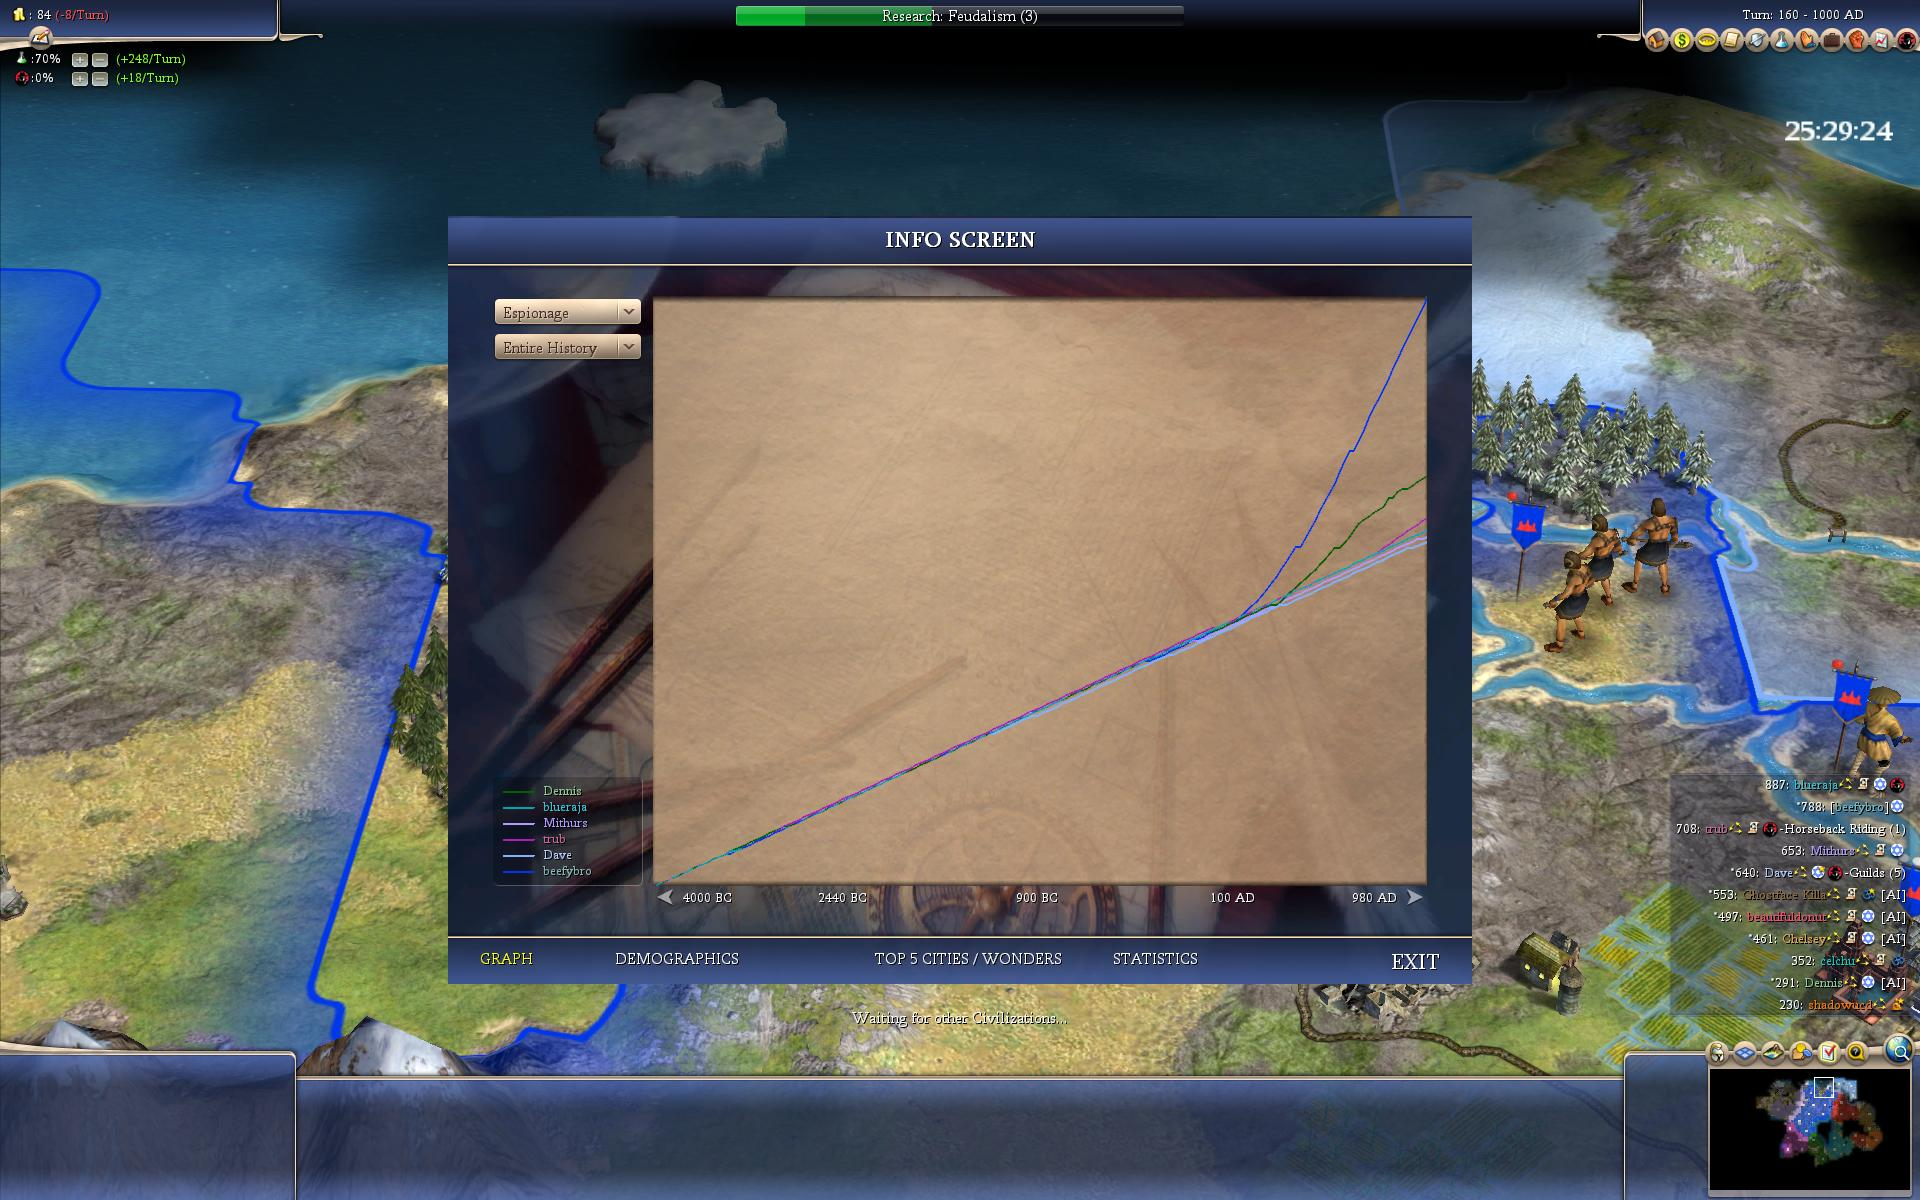
\includegraphics[width=1.0\textwidth]{turn160-3}

It's astonishing that Drew and Pat, despite having large empires, have
not built a single courthouse! It goes to show how IMBA the financial
trait is that they could get away with such a gross oversight and
still have healthy economies.

The site of my next city will be here:

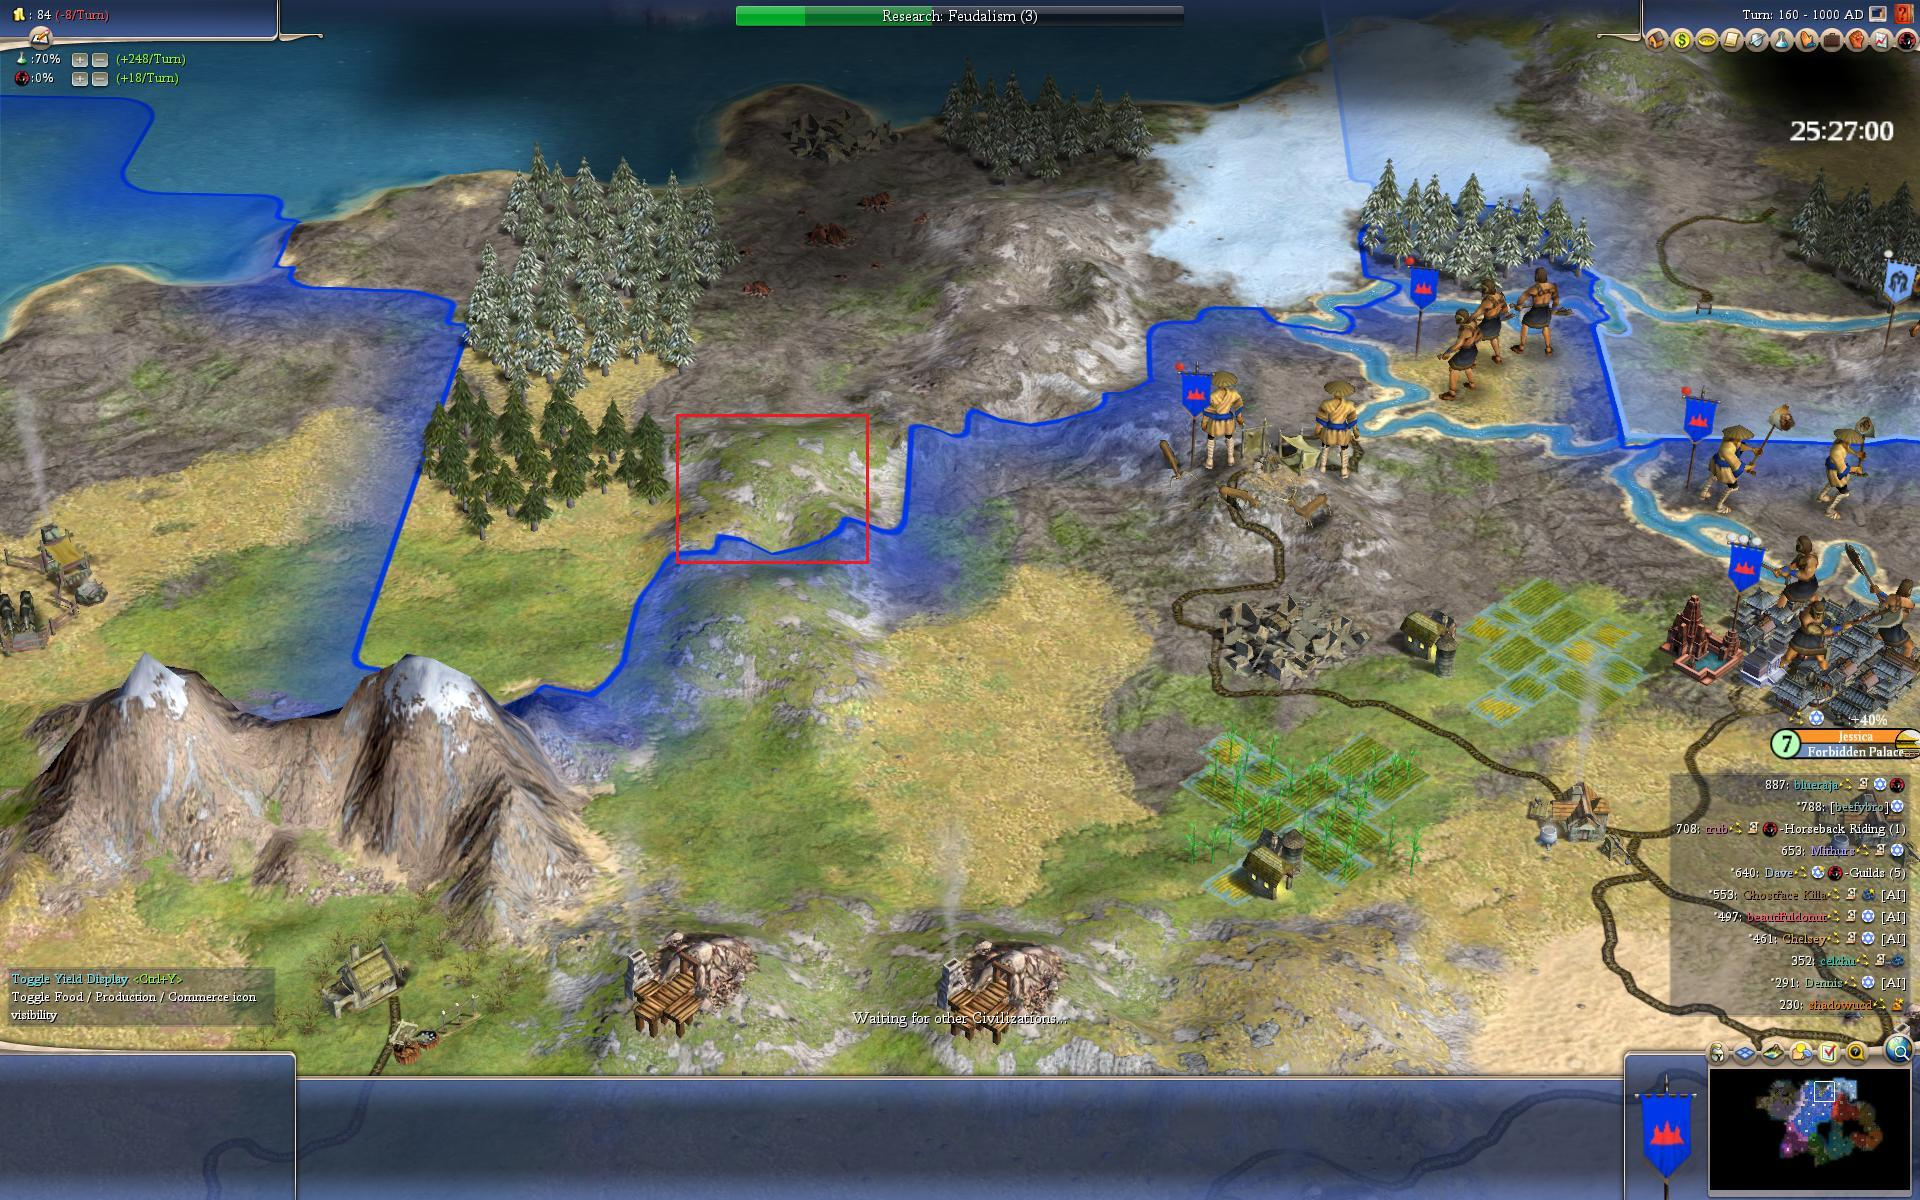
\includegraphics[width=1.0\textwidth]{turn160-4}

With biological farms and lumbermills, this could be an epic production city in the late game.

With no hope of winning Aaron, Lynda, Brad, and Chelsey have all given
control of their civs to the AI. I went ahead and ended the war with
Aaron since I wasn't going to get much more out of it and the AI was
willing to pay me 20g for peace. With these recent developments, Pat
is in an even better position than before; his neightbors consists of
2 warring AIs (Lynda and Brad), one crippled AI (Aaron), and two
crippled humans (Chris and Max). Hopefully DaveCop can expand out to
Pat and at least put a little pressure on him.

I'm still terrified about the effect the AP will have over the
game. All potential targets of mine are jewish, so I'll have to deal
with stop-the-war votes constantly. I can maybe cajole Drew into
voting my way with threats/bribes, probably DaveCop too. If DaveCop
converts to Judaism and converts more cities, that might give me
enough votes.

\section*{Turn 162}

Pat and I have reached a deal: I will vote him in as president, pay
him 2g/turn, and vote for all the proposals he raises as AP
president. Drew is unofficially on-board too, but I may have to extend
my side of the NAP to seal the deal.

I did some research into the AP in the event that Karmol wins the AP
election despite my efforts. 10 turns after the election, a proposal
can be made; *any* possible proposal can be raised. Every ten turns
after that, another proposal can be raised. After 4 proposals, another
election occurs. So, if I play things right, I'd have a 10-turn window
to take a city. I'd have to take a 10-turn break after that, but that
might be OK as it would give me time to heal and Karmol does not have
the productive capacity to build much in that time frame.

I had been improving the road network near Karmol to prepare for the
upcoming attack. He noticed the roads going up and correctly deduced
that I am preparing for an attack. This was a pretty huge mistake on
my part since I'm many turns away from attacking and the roads could
have waited. Even worse, Karmol was preparing an attack on Lynda/Brad
and his army would have been completely out-of-position to deal with
an attack from me (I can see all of Karmol's territory due to my big
spying advantage over him). Now, his sizeable (but mostly obsolete
stack: 6 cats, couple archers, swordsman, xbow, longbow) is defending
his capital. On the bright side, once this army and routed and capital
captured, Karmol is done.

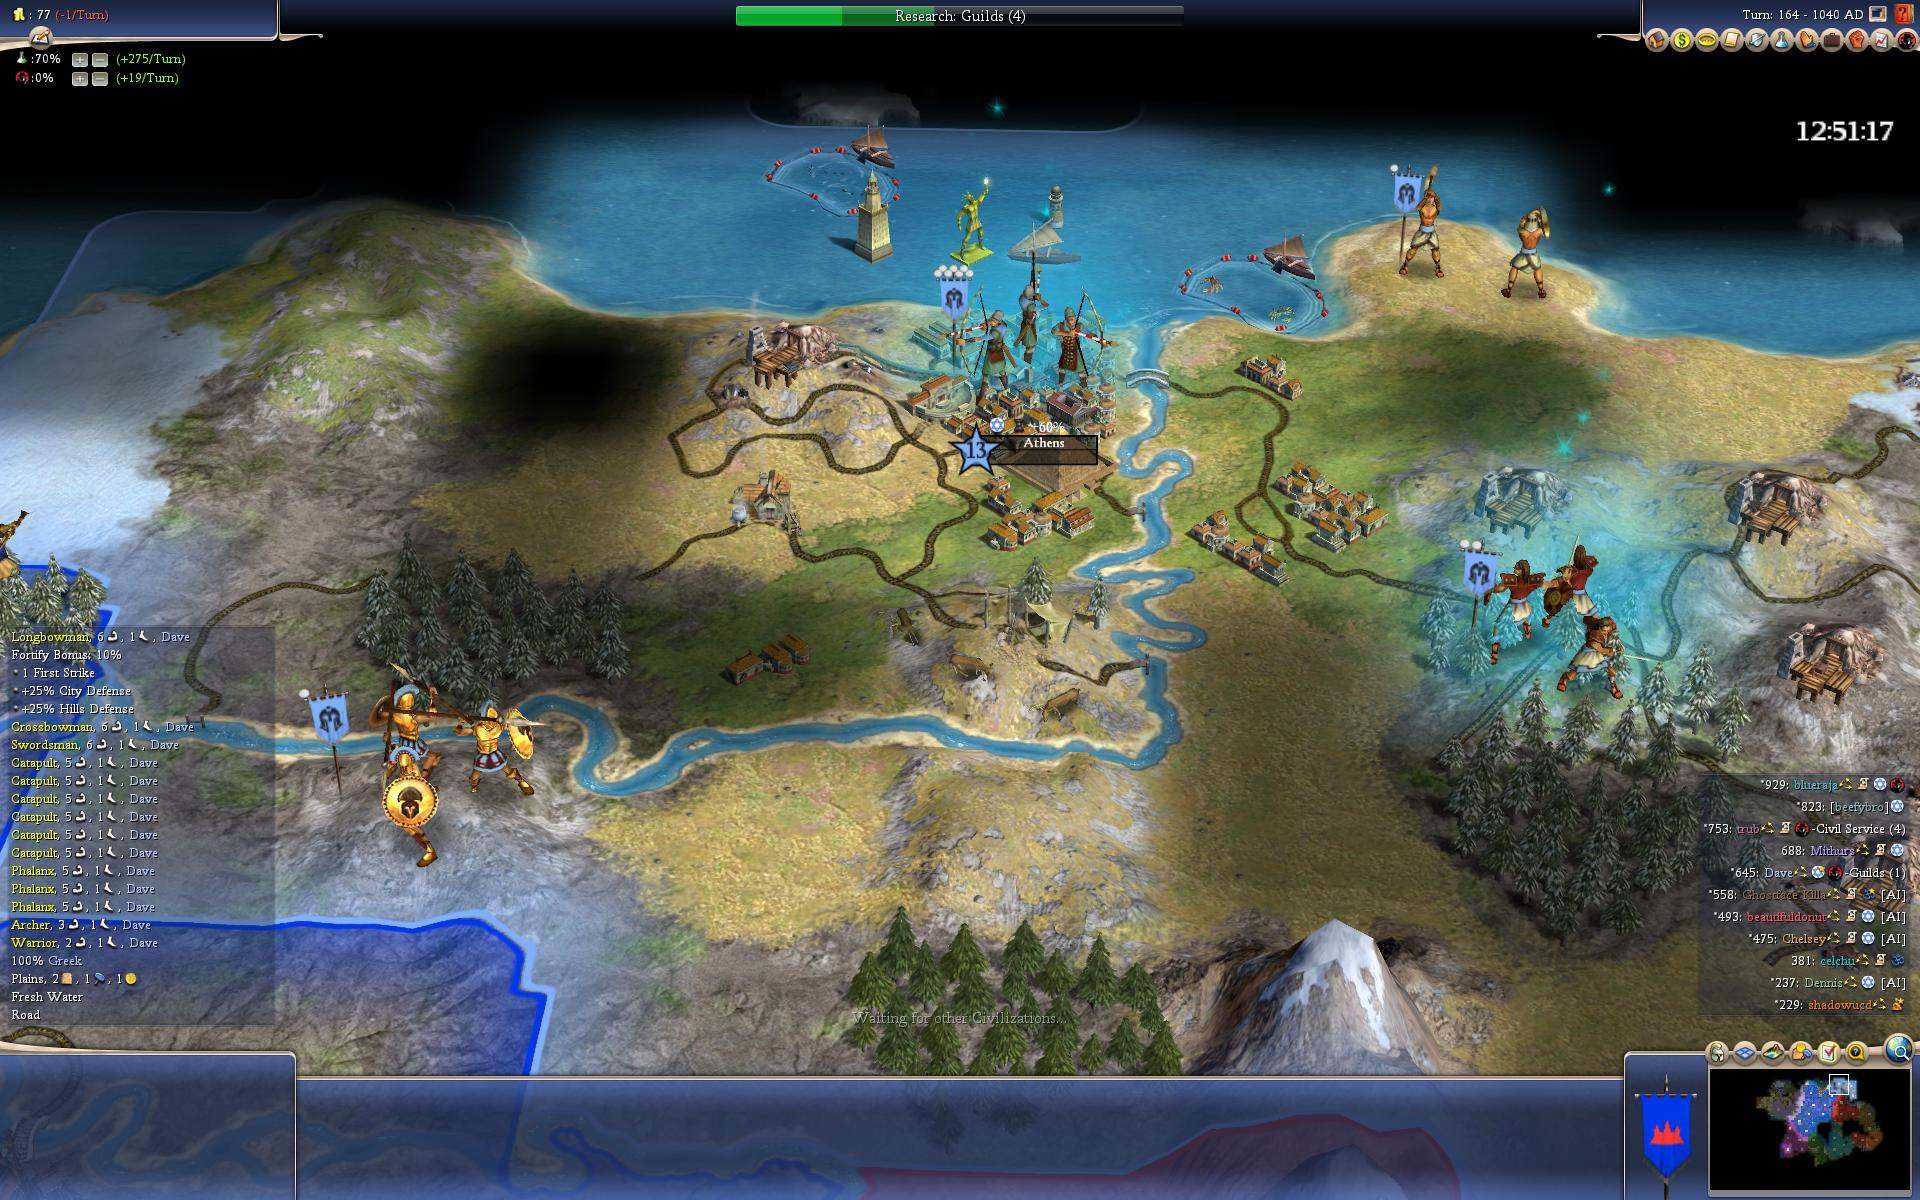
\includegraphics[width=1.0\textwidth]{turn164}

In order to get units faster, I should probably spend a few turns a
0\% science so I can upgrade my better axemen to maces. I should also
look for units that are defending cities that are no longer under any
threat, move them into position, and upgrade.

\section*{Turn 165}

I think I've found the perfect staging area to attack Karmol: the red
square in the screen shot below. With a road on the tile with the
axeman, I can get to the hills next to Karmol's capital in 3 turns and
he won't be able to see the stack.

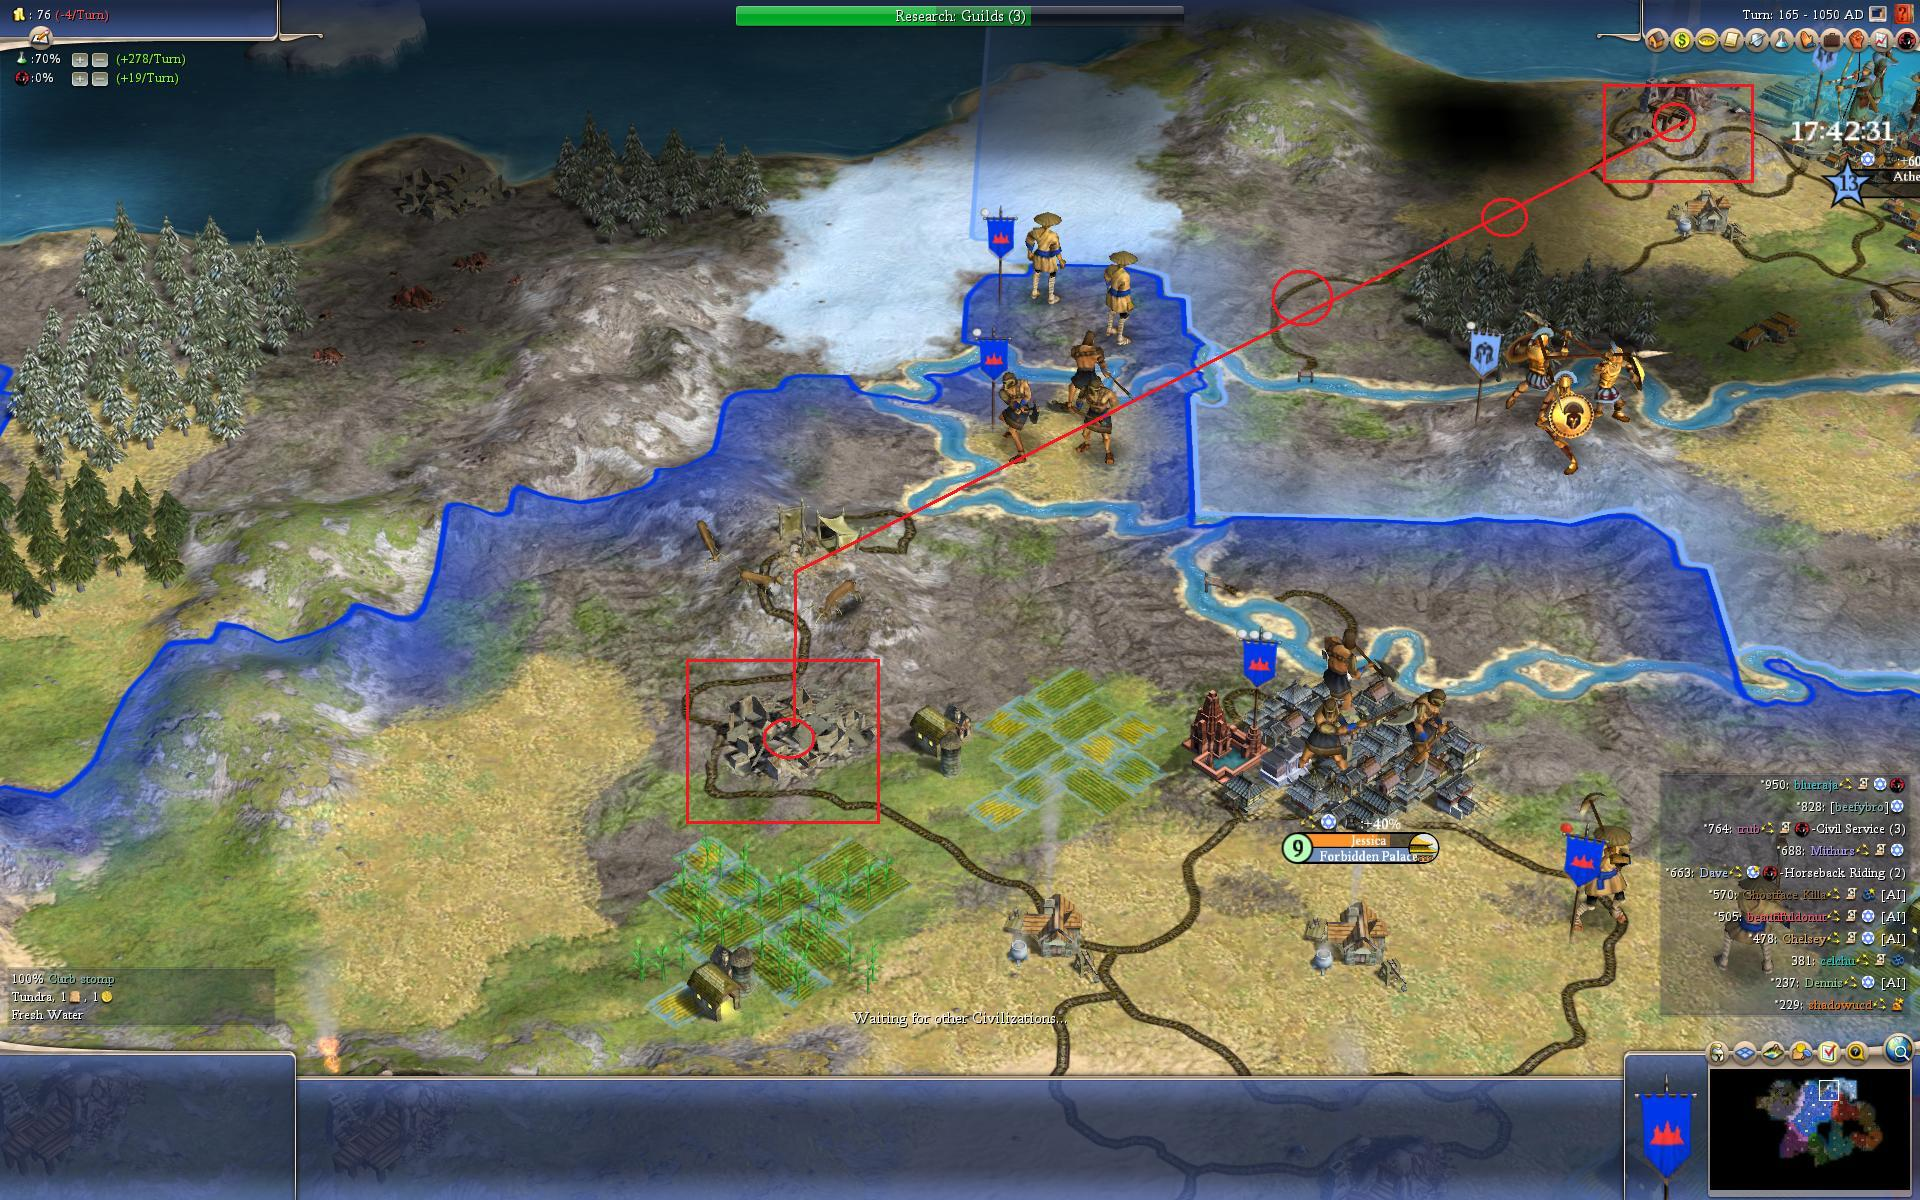
\includegraphics[width=1.0\textwidth]{turn165}

\section*{Turn 166}

I've had an idea for a major shift in strategy. Pat is probably going
for liberalism and he'll probably beat me to it even if I beelined
it. Instead, I may go for a powerful "monk" play instead: turn Jessica
into a massive production city by switching to caste system and use it
to pump a few key wonders: University of Sankore and Spiral
Minaret. With these two wonders and AP, a jewsish building would be
worth 2 science, 2 gold, 2 hammers. With cathedrals, temples, and
monastaries in key cities, that would be a bonus of 6 science, 6 gold,
and 6 hammers, worth approximately SEVEN specialists!! I think this
would make me extremely powerful and in runaway position if I can
capture Karmol's jewish-founding city. Making this even more
attractive is that Sankore and Minaret both build faster with stone,
which I have. It should also catch the other players off guard.

I need to meta Pat into thinking I'm challenging him for the
liberalism beeline. I also need to convince people that the war
against Karmol is the only Ace up my sleeve.

\section*{Turn 174}

Karmol has finally completed the AP; most of my cities have
monastaries, but few have temples since happiness has not been a
problem. I'm still massing troops for the battle with Karmol, so the
temples will have to wait for now.

A crucial deal I was making with Pat has fallen through... I had been
trying to negotiate a deal where I would make him pope for life in
exchange for a promise that he would not stop my wars against jewish
players. Now that this deal is dead, I'm going to have to be very
smart about when I launch attacks; if I time things right, I'll have
10 turns to take a city before the war is stopped. Karmol's capital
would be the first city of his to fall, so that would basically knock
him out of the game. I definitely think it can be taken in 10 turns
since I can get to its doorstep in 3 and I'll have a lot of siege
units to help. Right now, I have 6 trebs, 3 maces, 2 pikes, and 2
knights. This is not enough, so I'll have to wait 10 turns until the
next window. By then, with gold hoarding for upgrades, I should have
10 trebs, 7 maces, 2 pikes, and 6 knights; a balanced and formiddable
force.

My demographic position continues to decline and Pat and DaveCop are skyrocketing.

\section*{Turn 176}

Karmol won the AP vote and finished the statue of Zeus. Pat is
beginning to gobble up Lynda and is approaching runaway status. I
could try to form a voting bloc with Drew and DaveCop, but I don't
know if we'd have the votes to block a stop-the-war vote.

\section*{Turn 180}

University of Skankwhore built! My first wonder of the game... Work
has begun in Jessica on the Spiral Miranet.

I'm going to take another unusual path (for me) in the tech
tree. Music will give me a free great artist and allow me to make
uber-cathedrals (+3 happy, +2 hammer, +2 research, +2 gold, +50\%
culture).

At the moment I'm stockpiling gold for unit upgrades for the attack on
Karmol. The attack launches on turn 185!!

\section*{Turn 183}

Japan wanted to vassalize to me. Tempting, but not gonna happen. It
would start the war with Karmol too early, allowing him to block it,
and put me at war with Pat which I really don't want at the
moment. Aaron was finally eliminated.

\section*{Turn 184}

Attack begins next turn! Screenshots below reveal the situation

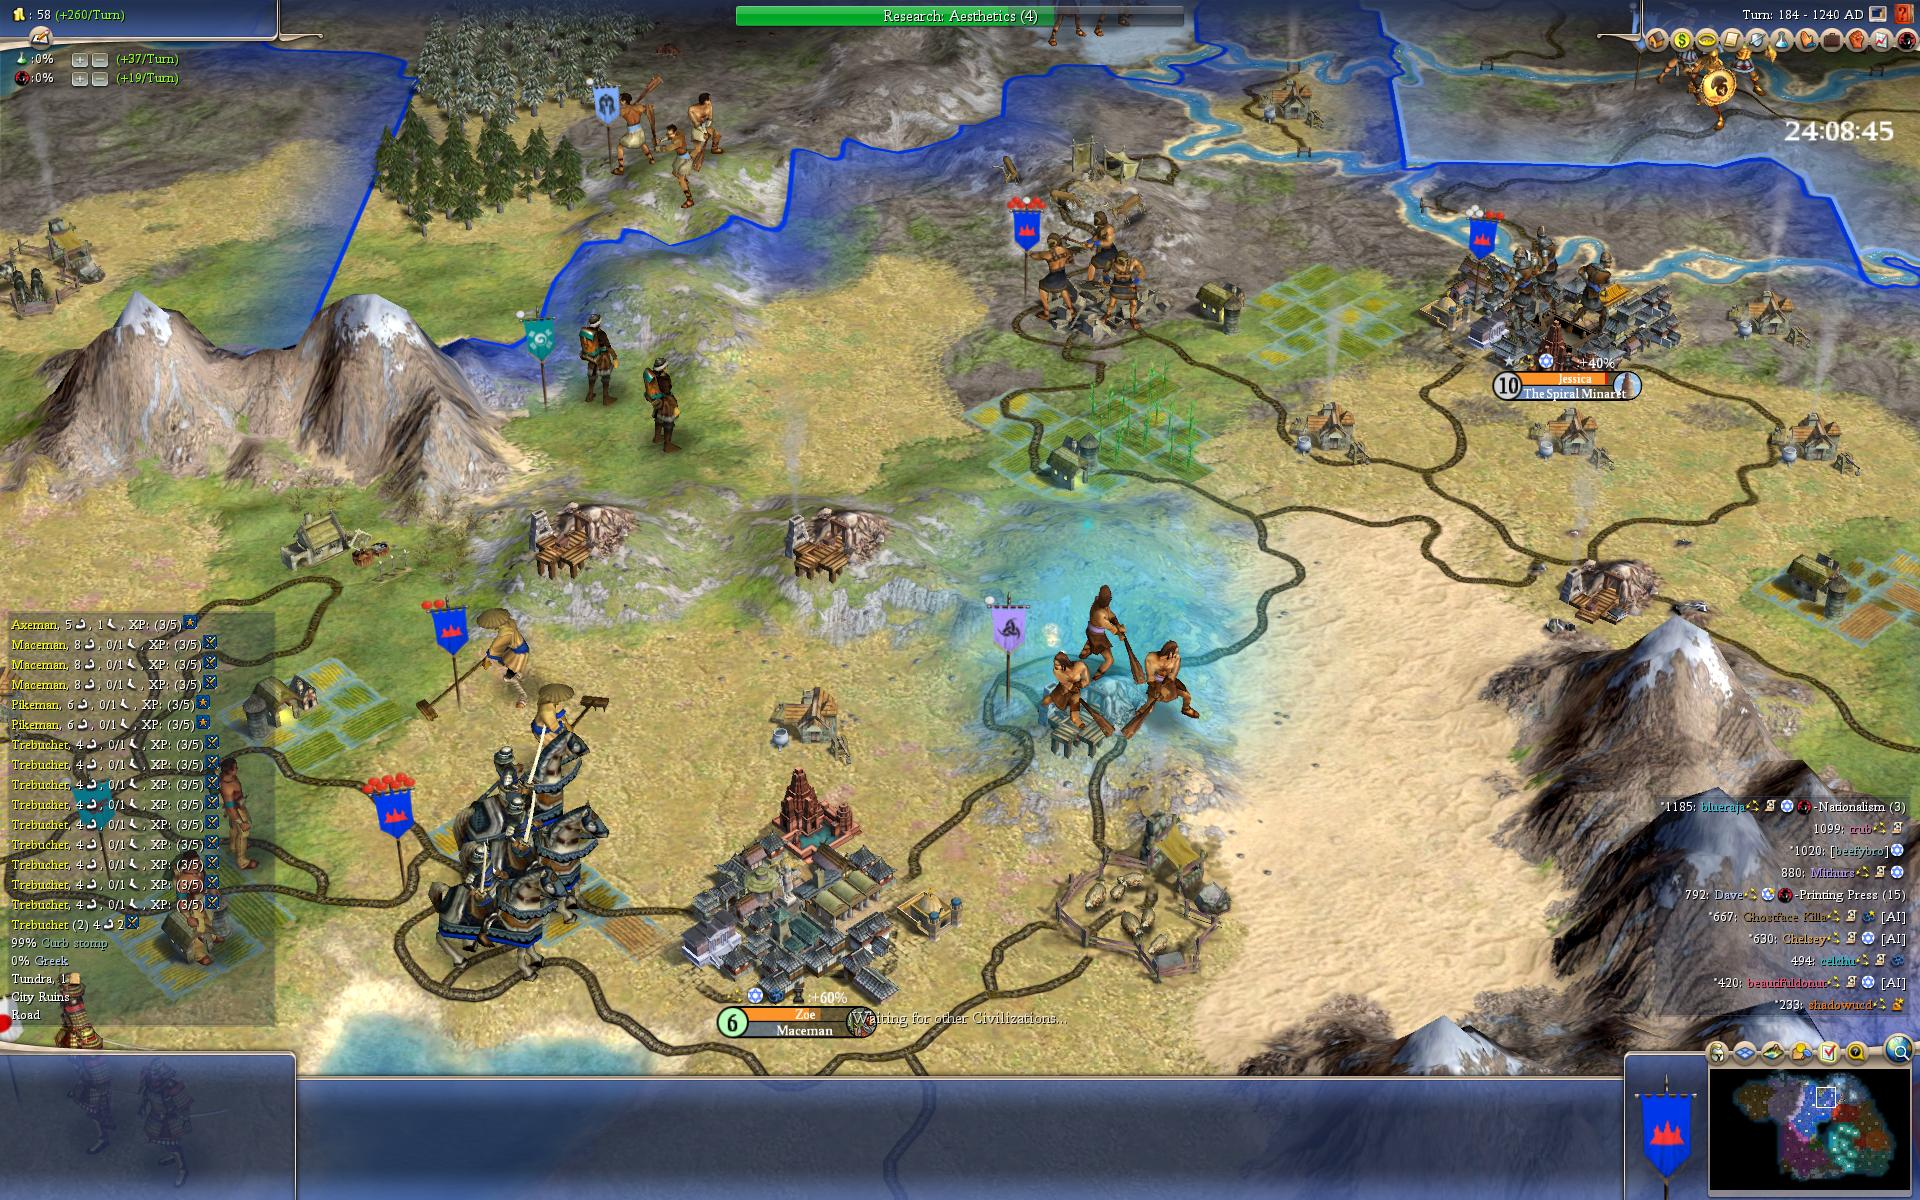
\includegraphics[width=1.0\textwidth]{turn184-1}
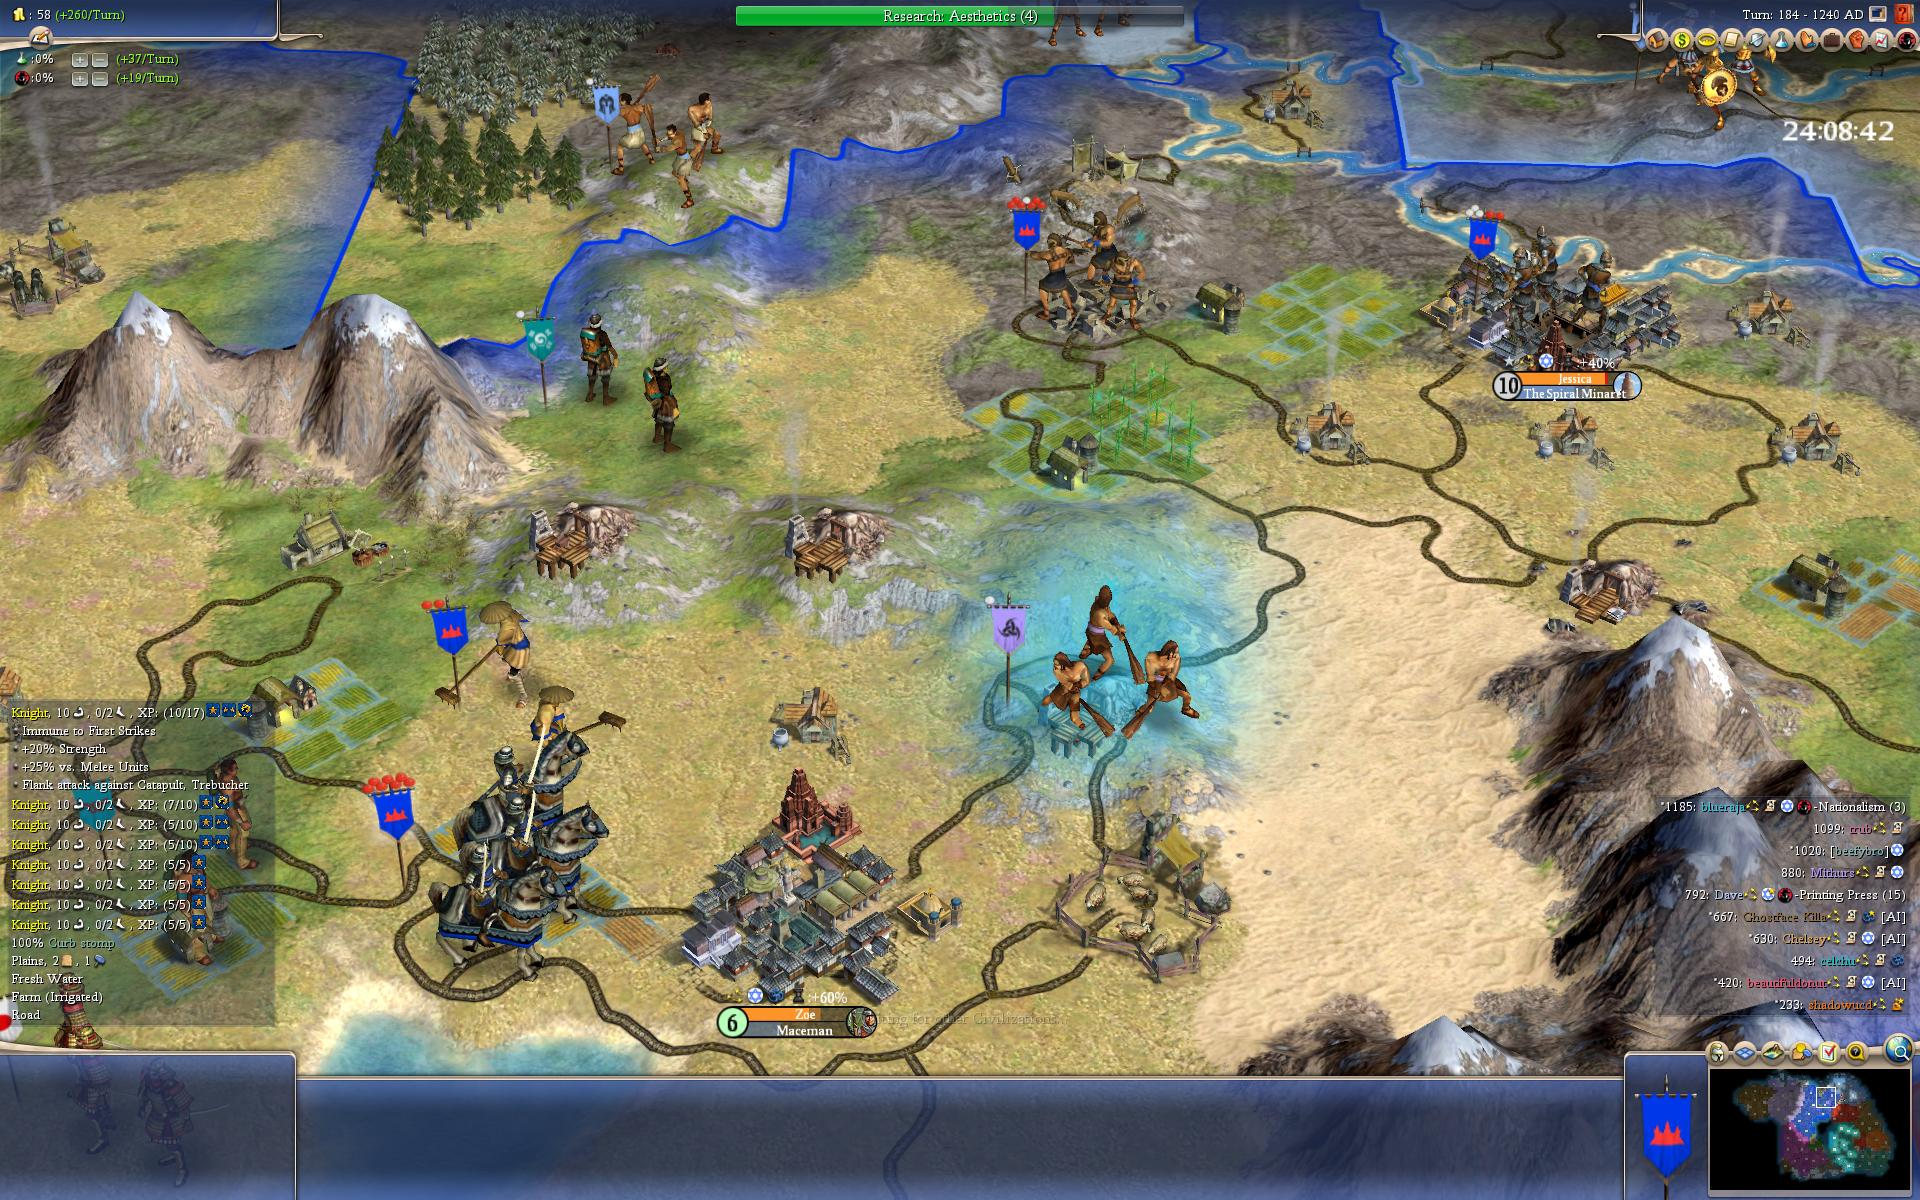
\includegraphics[width=1.0\textwidth]{turn184-2}
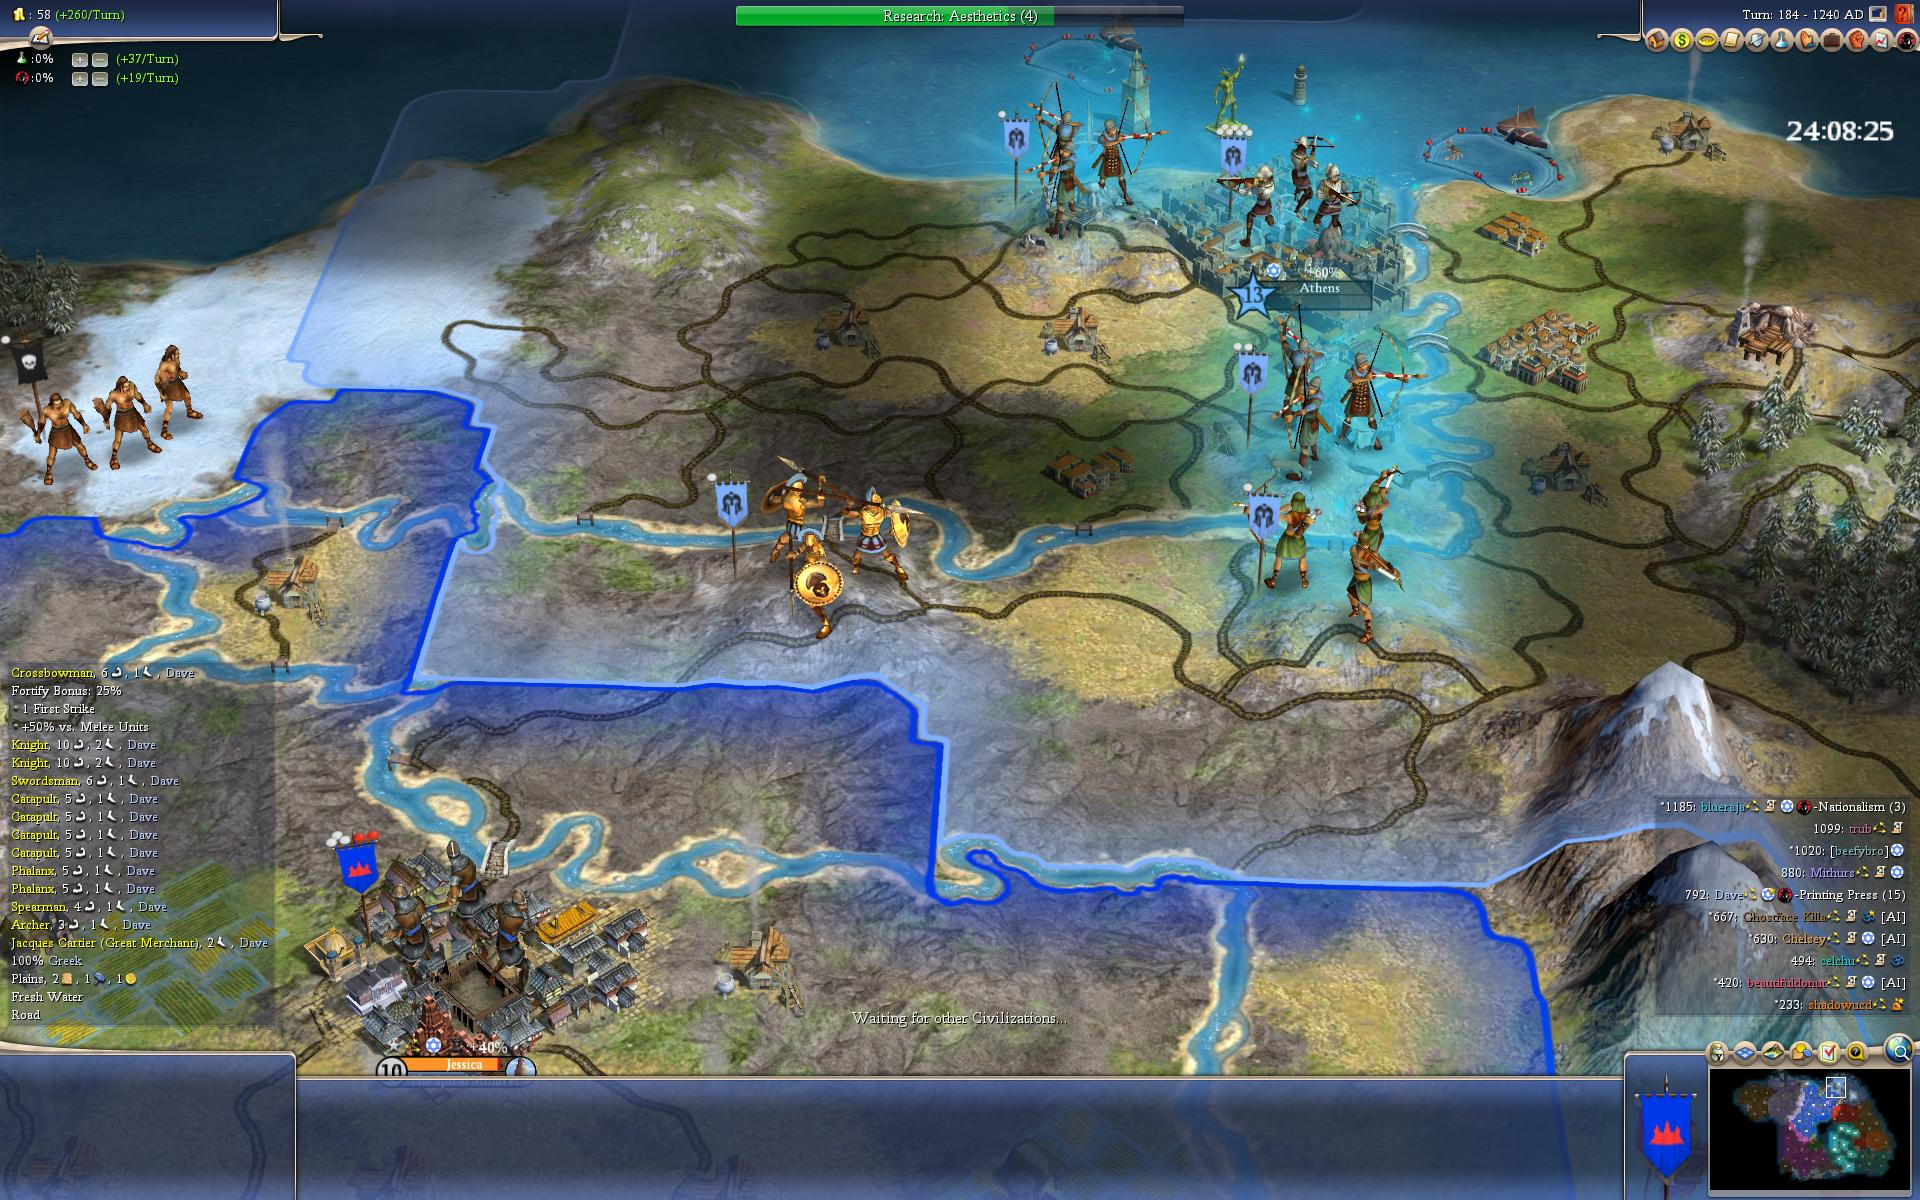
\includegraphics[width=1.0\textwidth]{turn184-3}

Karmol has taken Tokyo from Japan, but leaving his capital even less
defended than it was before. This should be an easy win unless Pat
feeds him a bunch of units. I should initially leave my knights in
Jessica, forking Karmol's force in Japan. He'll want to retreat to
save his capital, but he'll want to protect his new conquest as well.

\section*{Turn 185}

This is the turn that changed everything!

I went before Karmol this turn, declaring war on him, and positioning
my troops for an attack on his capital. In the process, I killed a
warrior and maceman without taking any losses. The next day, I was
shocked to see that Karmol was able to call a "stop-the-war" vote on
himself; simultaneously, Drew and Pat closed all trades with me (and
presumably voted Karmol's way). In a fit of rage, I selected "defy"
without really thinking things through. The loss of happiness
resources from Pat and Drew plus the -5 penalty for defy would have
put key cities deep into unhappiness, essentially bringing my economy
to its knees. Once I realized how badly things had turned in the span
of one turn, I retired from the game.

I ended up swallowing my pride and asking for a server reload on the
grounds that the AP mechanics were sufficiently unclear in pitboss
that I did not "deserve" to get so utterly destroyed by
misunderstanding them. The other players resisted this proposal and we
ended up reloading only my defiance, but my war against Karmol remains
blocked. Oddly enough, in subsequent turns, I never saw the results of
the vote and Karmol and I voluntarily signed peace; I still have yet
to figure out exactly what happened. Suffice it to say that I do not
understand the AP and I don't want to continue to worry about it, so I
made a deal that will drastically change the course of the game. I
have entered into an agreement with Pat and Karmol; the basic deal is
that I will agree to not attack Karmol and attack Drew instead in
return for no interference from the AP. Along with this deal comes an
indefinite NAP with Karmol and a 20-turn NAP with Pat.

Attacking Drew is not going to be easy; he's got a large empire and we
share a long border with each other. Unlike Karmol, the optimal
tactics are not obvious, but I will probably send the vast majority of
my forces due west into his core cities, sending just a couple units
north to threaten his spice city. Drew's army is weak, but he's in the
process of building units to attack Mongolia. He's also in slavery, so
he'll probably go into panicked whipping mode as soon as he realizes
what's going on.

This war will be more difficult and not as profitable as the war with
Karmol, but, looking back on it, a victory in the war against Karmol
would have been likely to draw a pile. Kuan said that Drew and Cop
were even going consider breaking their NAPs with me if I took over
Karmol! I can conquer Drew without making anyone unhappy at least and
he does have much more land than Karmol. Hopefully I can destroy his
main army and take his land quickly. Drew and I have had good
relations since our early wars, but I was disappointed in how quick he
was to sell me out during the drama with the AP vote; that made this
decision all the easier. This also serves to bring Pat and I closer
diplomatically, but it also leaves me without much way of keeping him
in check as he approaches runaway when he completes the taj mahal.

Pat is going to hit liberalism and there's not a damn thing I can do about it.

Cop and I have agreed to exchanged a buddist missionary for a islamic missionary.

The Spiral Miranet is complete and has given a significant boost to my
economy. Jessica has turned into a production monster with all that
food and workshops. Who says you need hills to be productive. As a
side note, I probably wouldn't even be in the game if I had let Karmol
have this city.

I will be the first to get Music, which will give me a great artist to be used for a golden age whenever I might need it.

Due to a massive espionage advantage, I can see what Pat is building in all his cities.

\section*{Turn 189}

Thanks to fast-moving knights, I'm just one turn away from beginning
my war against Drew. Once again, I'm catching him his pants down as he
has no strong defending units and no spears/pikes to counter the
knights. Even better, Drew is running caste system, so he can't go
into whip panic without having a revolution first! It's possible that
Drew may be an easier target than Karmol was! An example of complete
lack of strong defenders:

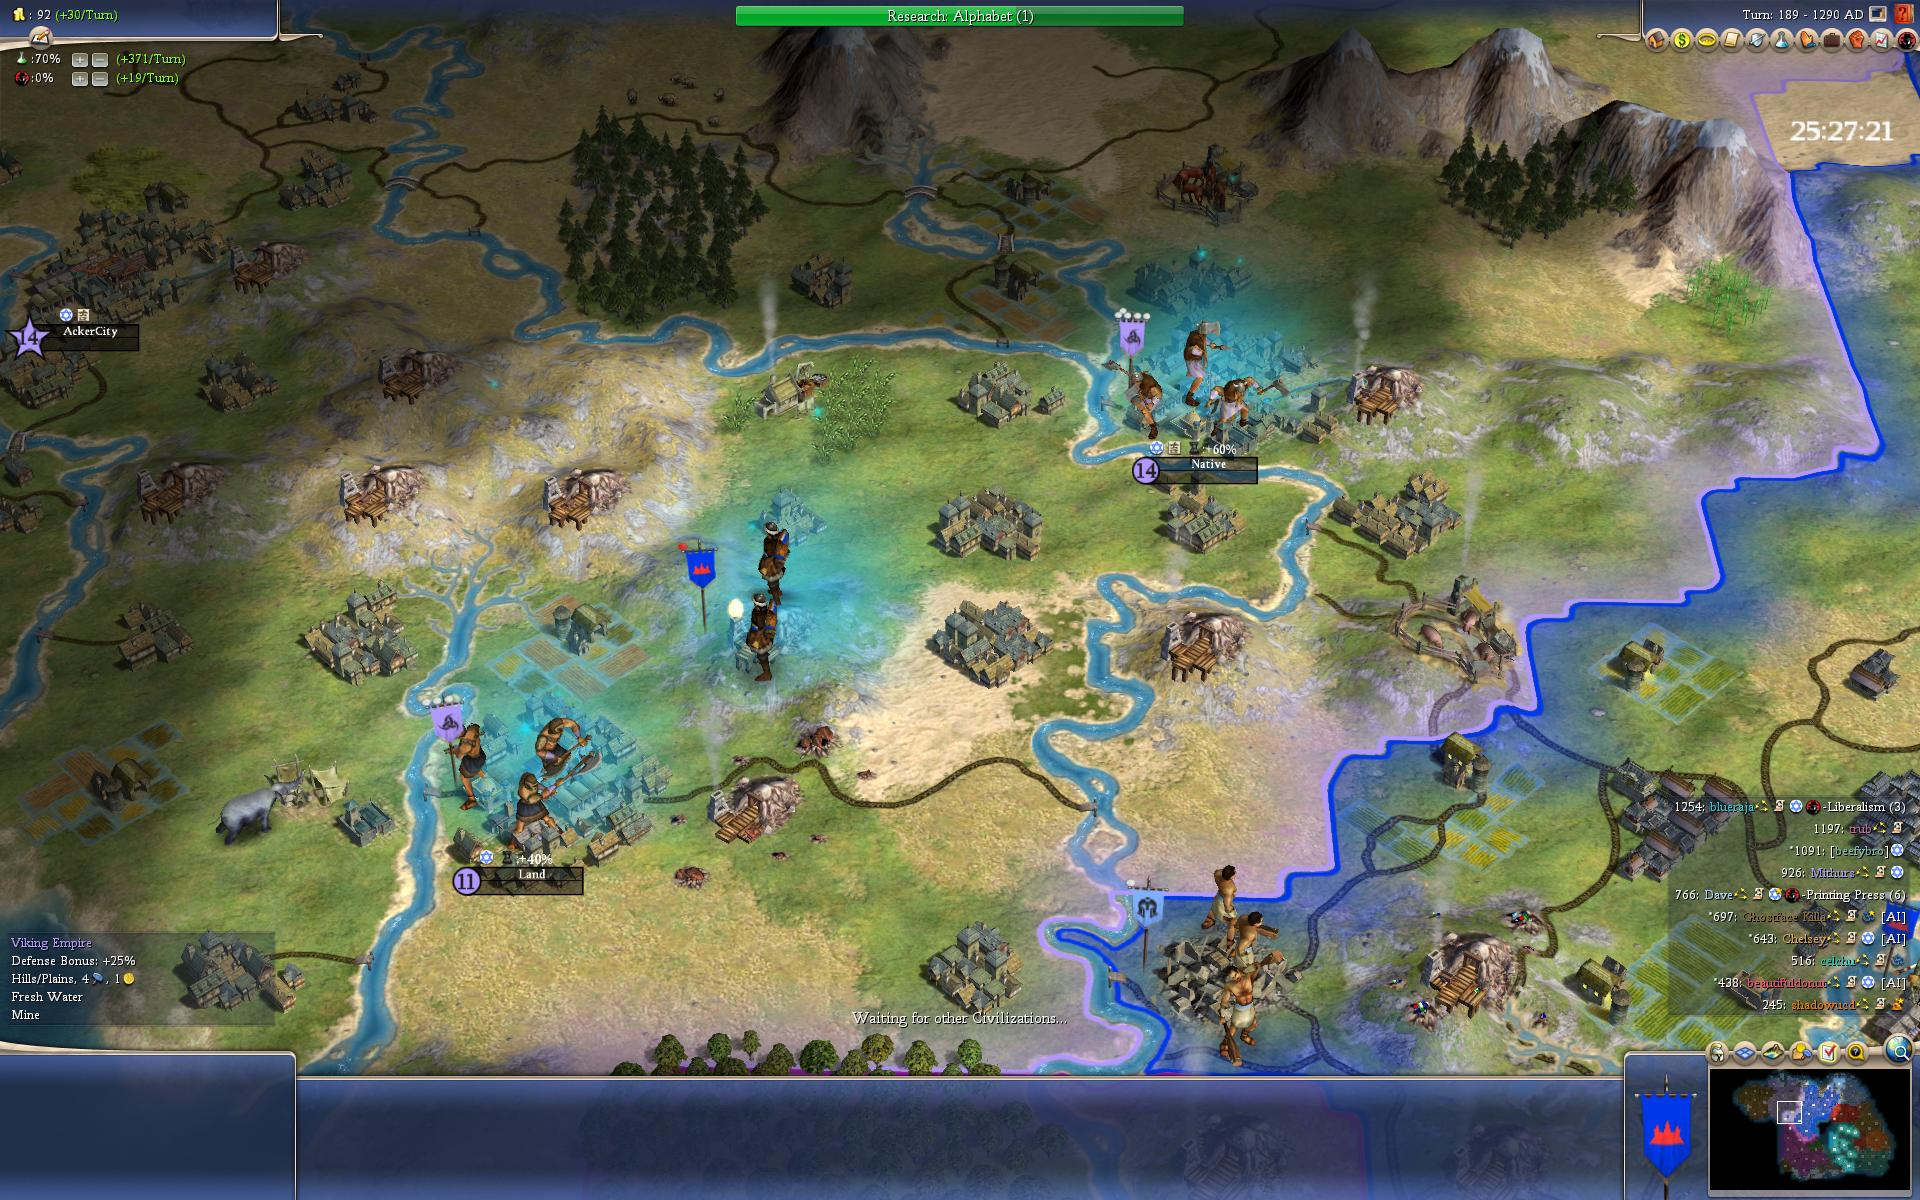
\includegraphics[width=1.0\textwidth]{turn189}

My demographics have rebounded a bit due to the wonders and the fact that I'm researching an easy tech:

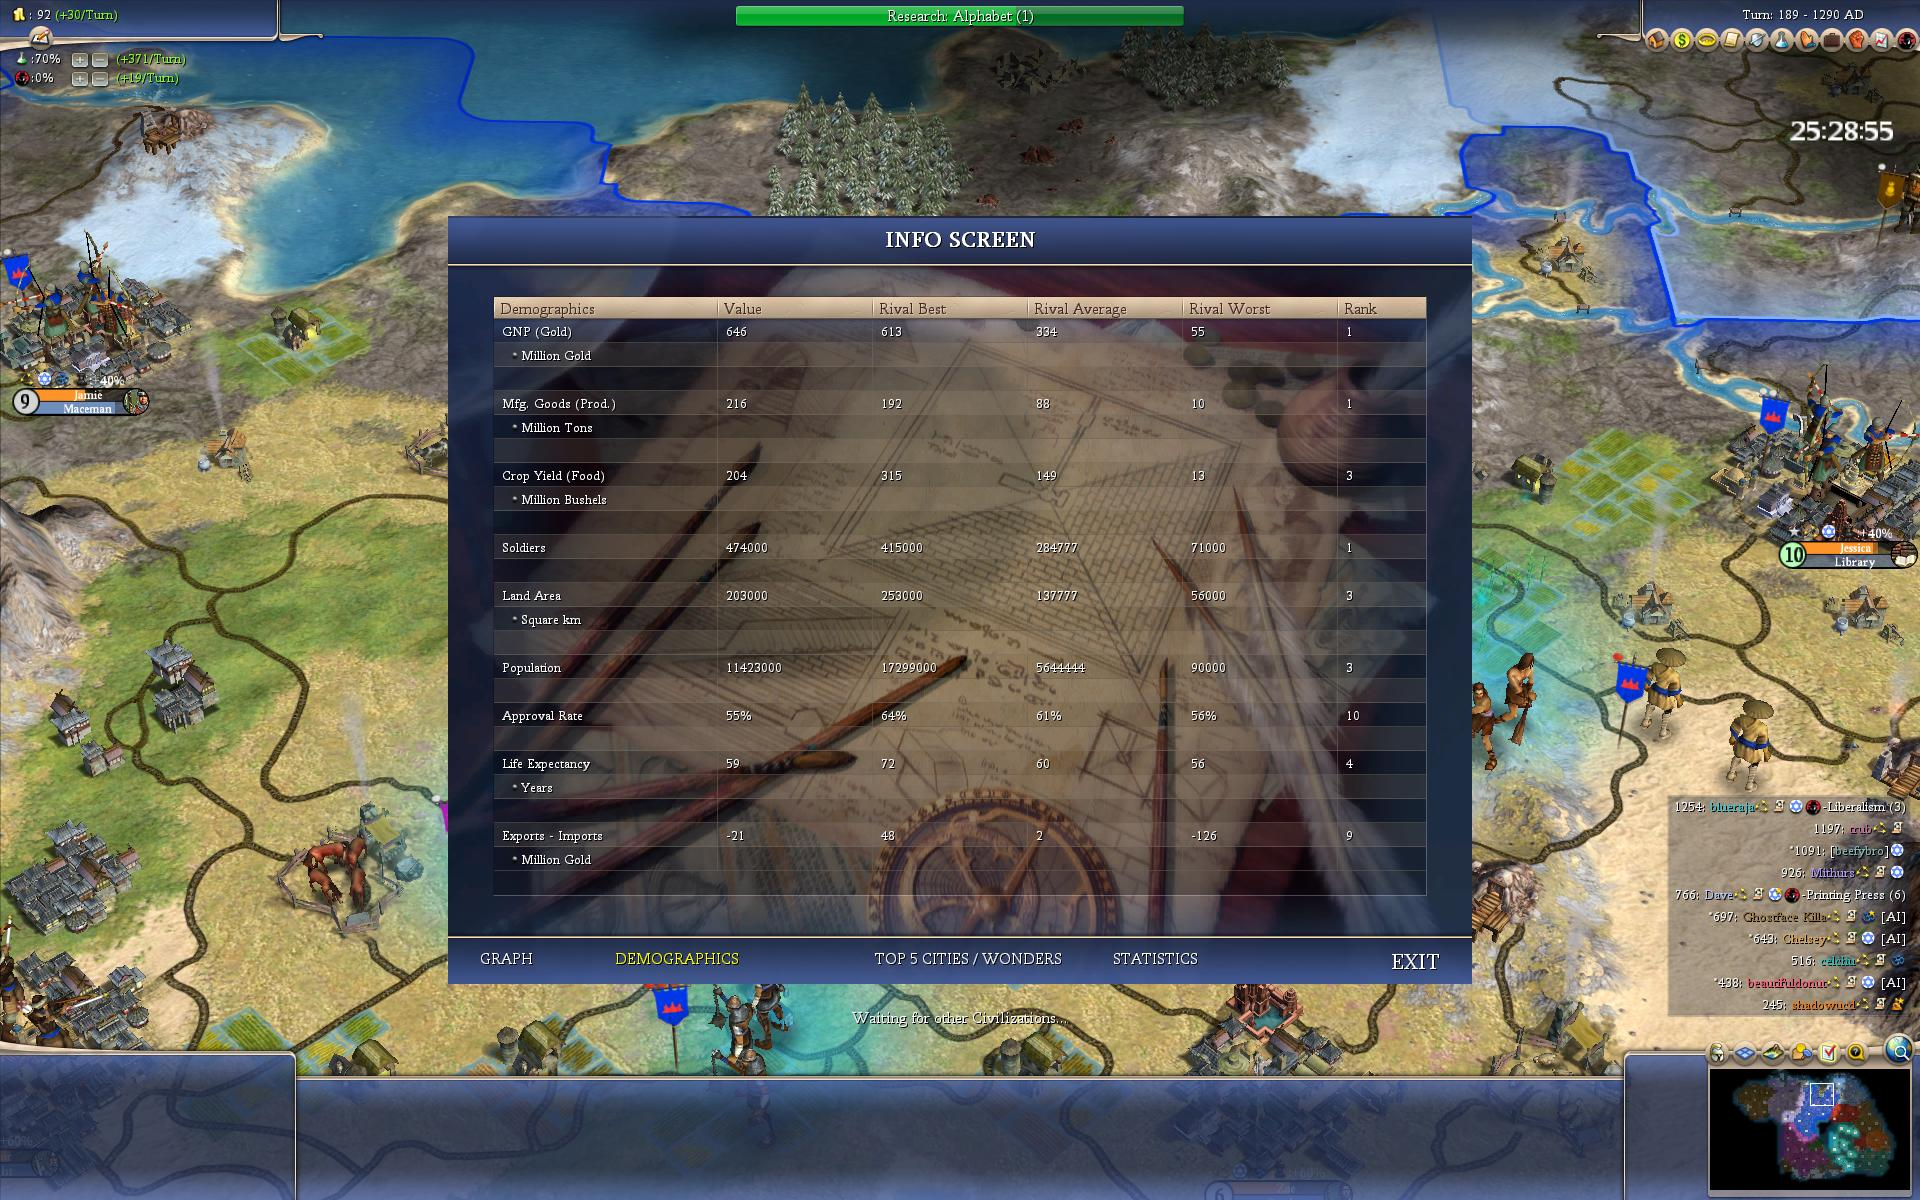
\includegraphics[width=1.0\textwidth]{turn189-2}

Pat continues to have a massive lead in food, although that's been the
case for quite a while now and he hasn't been able to translate it
into a GNP and MFG lead yet. It's possible that he overbuilt farms.

Apparently, Brad beelined music aeons ago, so I got no great artist
:(. On the bright side, those synagogues are going to be really nice
with the Sankwhore and Miranet bonuses. The +3 happiness + notre dame
should ensure that happiness is not an issue for the rest of the game.

I've decided to get printing press before education since it's bonus
will be instant. That will give me time to make units and build
synagogues etc. Education will come right after. The techs after that
will depend on how the war with drew is going and what techs Pat is
getting. The one thing that is totally unacceptable is for Pat to have
rifles with me stuck with medieval units.

\section*{Turn 190}

The diplomatic situation continues to thrash wildly. Drew was able to
get some anti-mounted units in his nearest city to me, so I can either
take the city with heavy losses or wait for my main force to arrive in
3 turns. Neither option is good... knights are expensive and I don't
want to throw them away, but if I wait, he'll be able to get a large
number of units into the city since he switched to slavery.

Just as in our early war, it's clear that Drew knows more than enough
to make a war against him painful and a long, drawn-out war is the
last thing I need as Pat continues to surge. So, instead of pushing
ahead and giving Pat the win, Drew and I have formed an alliance even
while ostensibly at war, and we will try to launch a surpise attack
against Pat. DaveCop is an essential partner in this deal, here's the
email I sent to him:

"""
Hi Dave,

Here's the situation:

My attempt to put pressure on Pat by conquering
Karmol was thwarted by the AP fiasco. Shortly after, Pat came to me
with a deal involving papal support for a war with Drew in return for
a NAP between Karmol and myself, which I foolishly accepted. I
declared war on Drew last turn and we ended up having a long
discussion last night. As it turns out, Pat has been playing both
sides against each other. Further, I can see Pat's research and what
he's building in all his cities. His research rate is almost double
that of anyone else and he's just 7 turns from popping Taj Mahal,
giving him a 12-turn golden age due to his completion of the Mausoleum
earlier in the game. With this extended golden age, he will be able to
go deep into the renaissance techs in the blink of an eye, picking up
riflemen, democracy, etc; in other words, he will have run away and
there won't be a damn thing anyone can do about it (maces/knights
vs. riflemen would be very ugly).

What can we do? Turns out, not much without your help...

Here's what we need from you:

* Drew and I are going to pretend to be stuck in a quagmire war while
secretly marching units through your territory. We need you to allow
this to happen without alerting Pat, keeping us posted of any Greek or
Mayan scouts that may be in your territory.

* We need you to upgrade the large army you have in Nippur and send it
with us to help in the attack.

* We need you to convert as many cities as possible to Judaism and
switch to it as your state religion so that we can block any AP
proposals that may hinder our attack.

Here's what we can offer you:

* Drew has already closed borders with Mongolia, blocking their stack
from reaching you and removing any threat to your lands.

* I can run 0\% tech slider and feed you the gold you need to upgrade
as many units as possible

* I can feed you jewish missionaries to help convert your cities.

The potential for success is low if Pat is able to get rifles out. We
can only hope that the war between Drew and I will convince him to
pursue economic techs instead.

The most important decision of the game is here, will you join us?

-Jim
"""

Dave was receptive to this deal.

\section*{Turn 191}

A new plan against Pat:

"""
Hi Dave,

Sorry for another long email; here goes...

Drew and I talked today and we think we have a better plan to deal
with the Pat situation. The old plan involved a massive attack on Pat
with medieval units; while this could work, Pat is likely to have
riflemen and be in mid golden age by the time we get over there, so I
fear we'd just get routed.

Instead, here's the new plan.
\begin{itemize}
\item Drew and I will continue to pretend to be at war until he is at full force
\item We will make peace and I will gift my entire stack over to him
\item Drew will run a surplus big enough to keep me at 100\% science and gift me it
\item Drew will launch a massive attack on Karmol using us to block stop-the-war votes in the AP
\item Once I am back at tech parity with Pat, Drew will stop feeding me and I'll start to build a new army
\begin{itemize}
  \item Perhaps while doing this, I feed you and/or Drew so you guys can get to rifles faster
\end{itemize}
\item Then I hit pat with a modern army, hopefully with you and Drew joining in later
\end{itemize}

What we need from you is pretty simple, just develop your tech as fast
as possible and vote with us in the AP. Be ready to join us when your
NAP expires. We could also negotiate unit gifting.

-Jim
"""

\section*{Turn 193}

Drew and I have been laying tons of meta-game on Pat and it seems to
be working. Pat is getting confident to the point of offering to be
declared winner.

With Drew feeding me and great scientists starting to pump from
Jessica, I should be able to more-or-less keep up with Pat in
tech. Getting Statue of Liberty would be a nice boost as it's the best
wonder of this era. Democracy also enables some powerful espionage
buildings, so it would open up the possibility of getting more
aggressive against pat via spies.

\section*{Turn 202}

The situation is dire... Pat is 2 turns away from steel and his
manufacturing capacity is almost double mine:

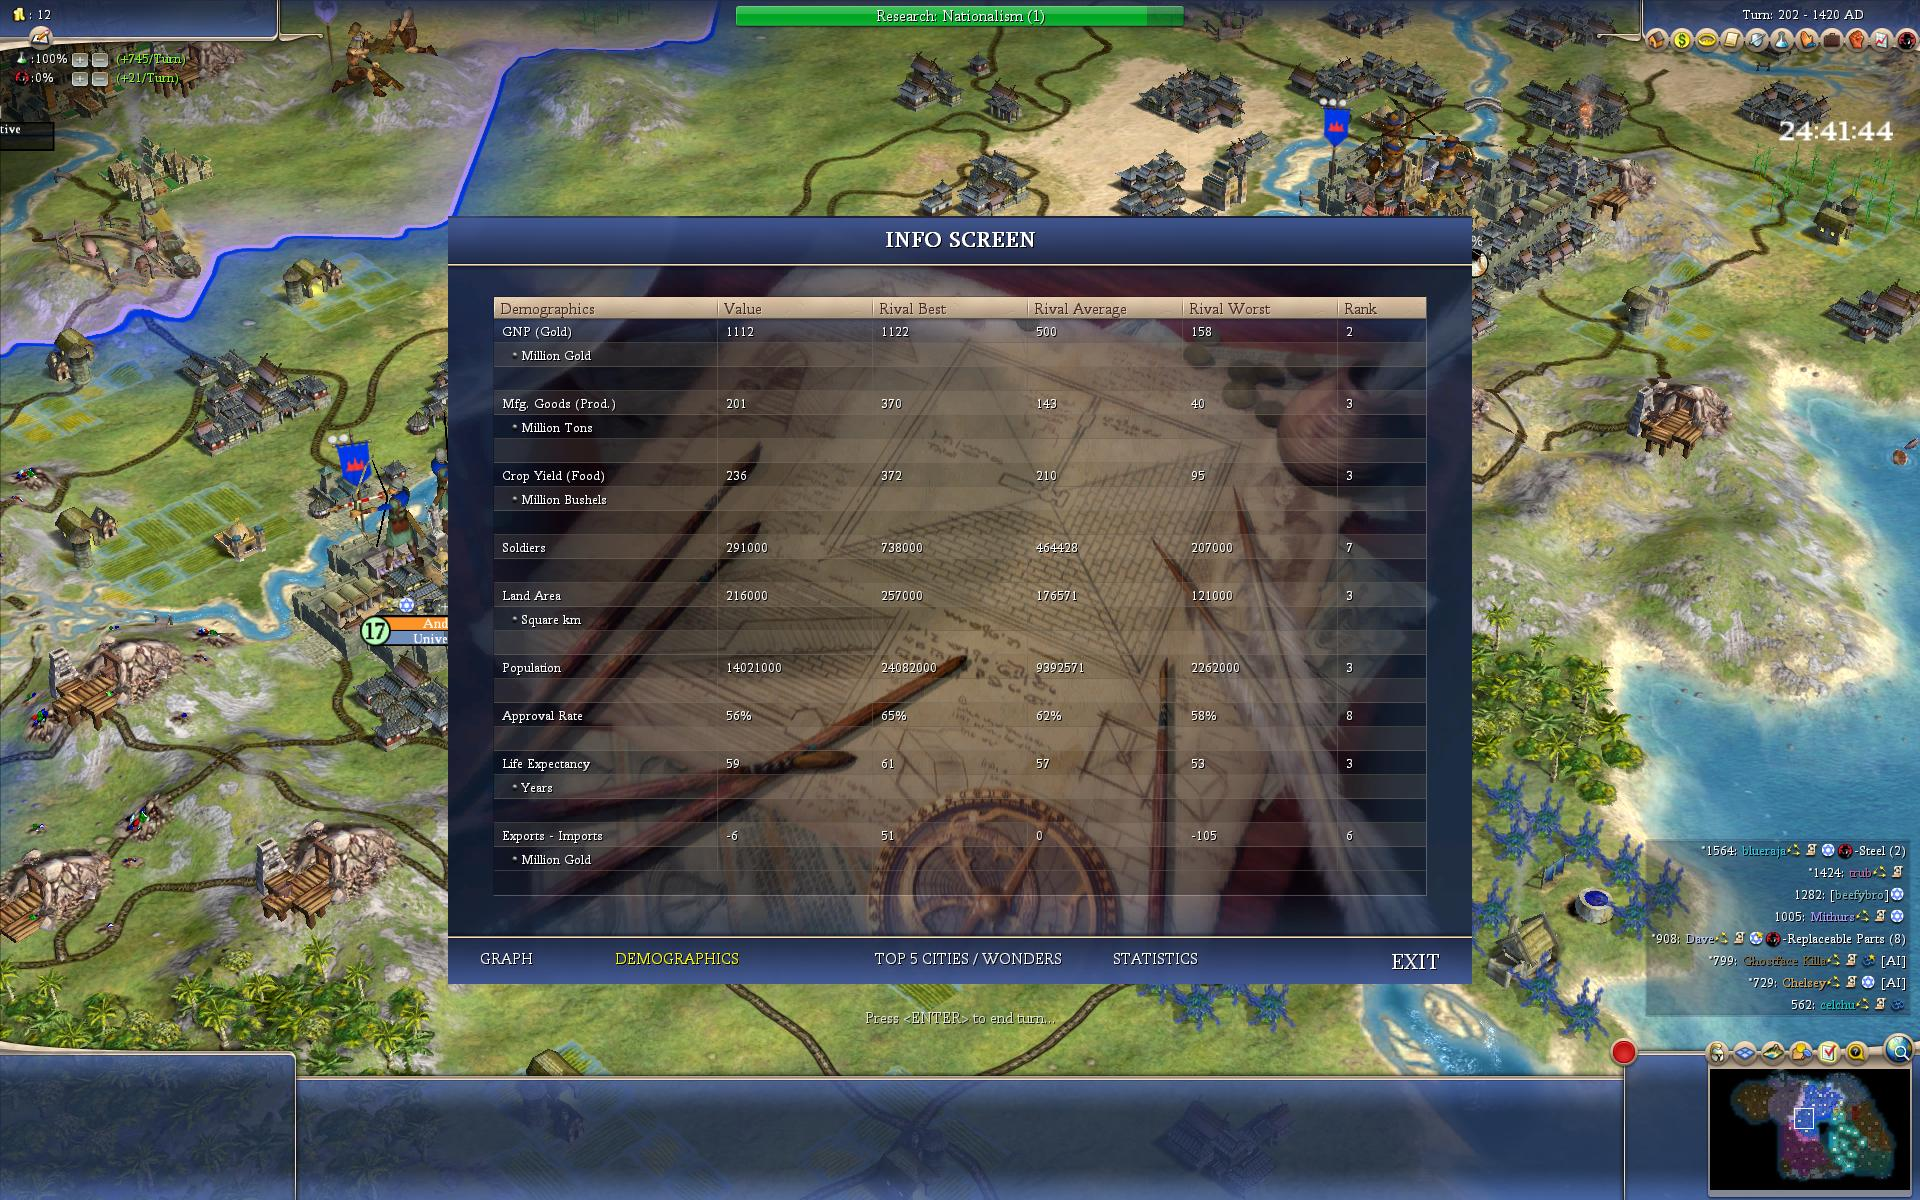
\includegraphics[width=1.0\textwidth]{turn202}

My economy is somewhat keeping up with his due to Drew's 82 gold/turn,
but Pat has at least 4 important techs on me and he has 20 or so turns
left of golden age.

There is only one path forward where Pat does not win easily in the next 30 or so turns:
\begin{itemize}
\item Drew takes over Karmol quickly before Pat can respond
\item I pop a golden age with my next scientist and put some economic pressure on pat
\item We all embargo Pat, putting some further pressure on his economy
\item Drew becomes pope, making any attack by Pat on us blockable.
\item With Pat worried about falling behind economically, he focuses on peaceful building instead of military.
\end{itemize}

With the NAP between Pat and myself expiring soon, I can't really
afford to completely neglect my military and need to reinforce
Jessica's defenses soon. Pat's army is nothing special yet, so
hopefully we have a 10 turn window or so due to production and move
time.

I sent another desperate plea to other players:

"""
Hi guys,

I think the game is basically over, but if we want to try to keep
things competitive, we need to embargo Pat as soon as possible (no
open borders, no resource trading). Losing most of his foreign trade
routes should at least slow his economy down a bit. This embargo will
only be effective if we're all on board.

Dave, we *really* need you to adopt Judaism as your state religion as
soon as you can so we can dominate the AP. I think Drew will be the
next pope if he can hold on to Karmol's capital long enough and then
we can slow Pat down with stop-the-war votes. This is the only
realistic future path where Pat doesn't have the game wrapped up the
next 30 turns.

I will pop a golden age in the next couple turns which should boost my
GNP well beyond Pat's. I *hope* this will scare Pat into focusing on
his economy more instead of building cannons (he has steel in 2
turns). If he makes a bunch of cannons and wipes Drew's force, the
game is over.

The situation is dire... Pat has powerful military techs that none of
us is close to getting and his manufacturing capacity is enormous, so
it would not take him long to build a large number of units.

If we don't stand together, coordinate/communicate, then we may as well retire and start game 5.

-Jim
"""

I really don't like being in the position of having to rely so much on
other players. DaveCop in particular has been difficult to work with
due to sporatic communication. I get the sense that he feels like I'm
as big of a threat to him as Pat, which is a little silly given the
current demographics. He seems to be dumping most of his espionage
points into me which is a complete waste; we'll need all the resources
at our disposal, including spies, if we are to have any chance at
this.

I don't know if my plan to get democracy/statue-of-liberty is viable
given the desperate situation. It is true that letting Pat have SoL
would be a disaster, a huge military loss means the game is over.

\section*{Turn 206}

Drew captured Karmol's capital and Karmols score seems to indicate
that he's circling the drain (his score is just above Max's, 2nd to
last). There are lots of troops moving around in Karmols territory,
but nothing to threaten Drew except for a few cannons that Pat gifted
to Karm. With Drew's 50 units, it would take at least 12 cannons to do
lots of damage to a stack of that size and he'd risk losing lots of
the cannons unless they were well-defended by other units.

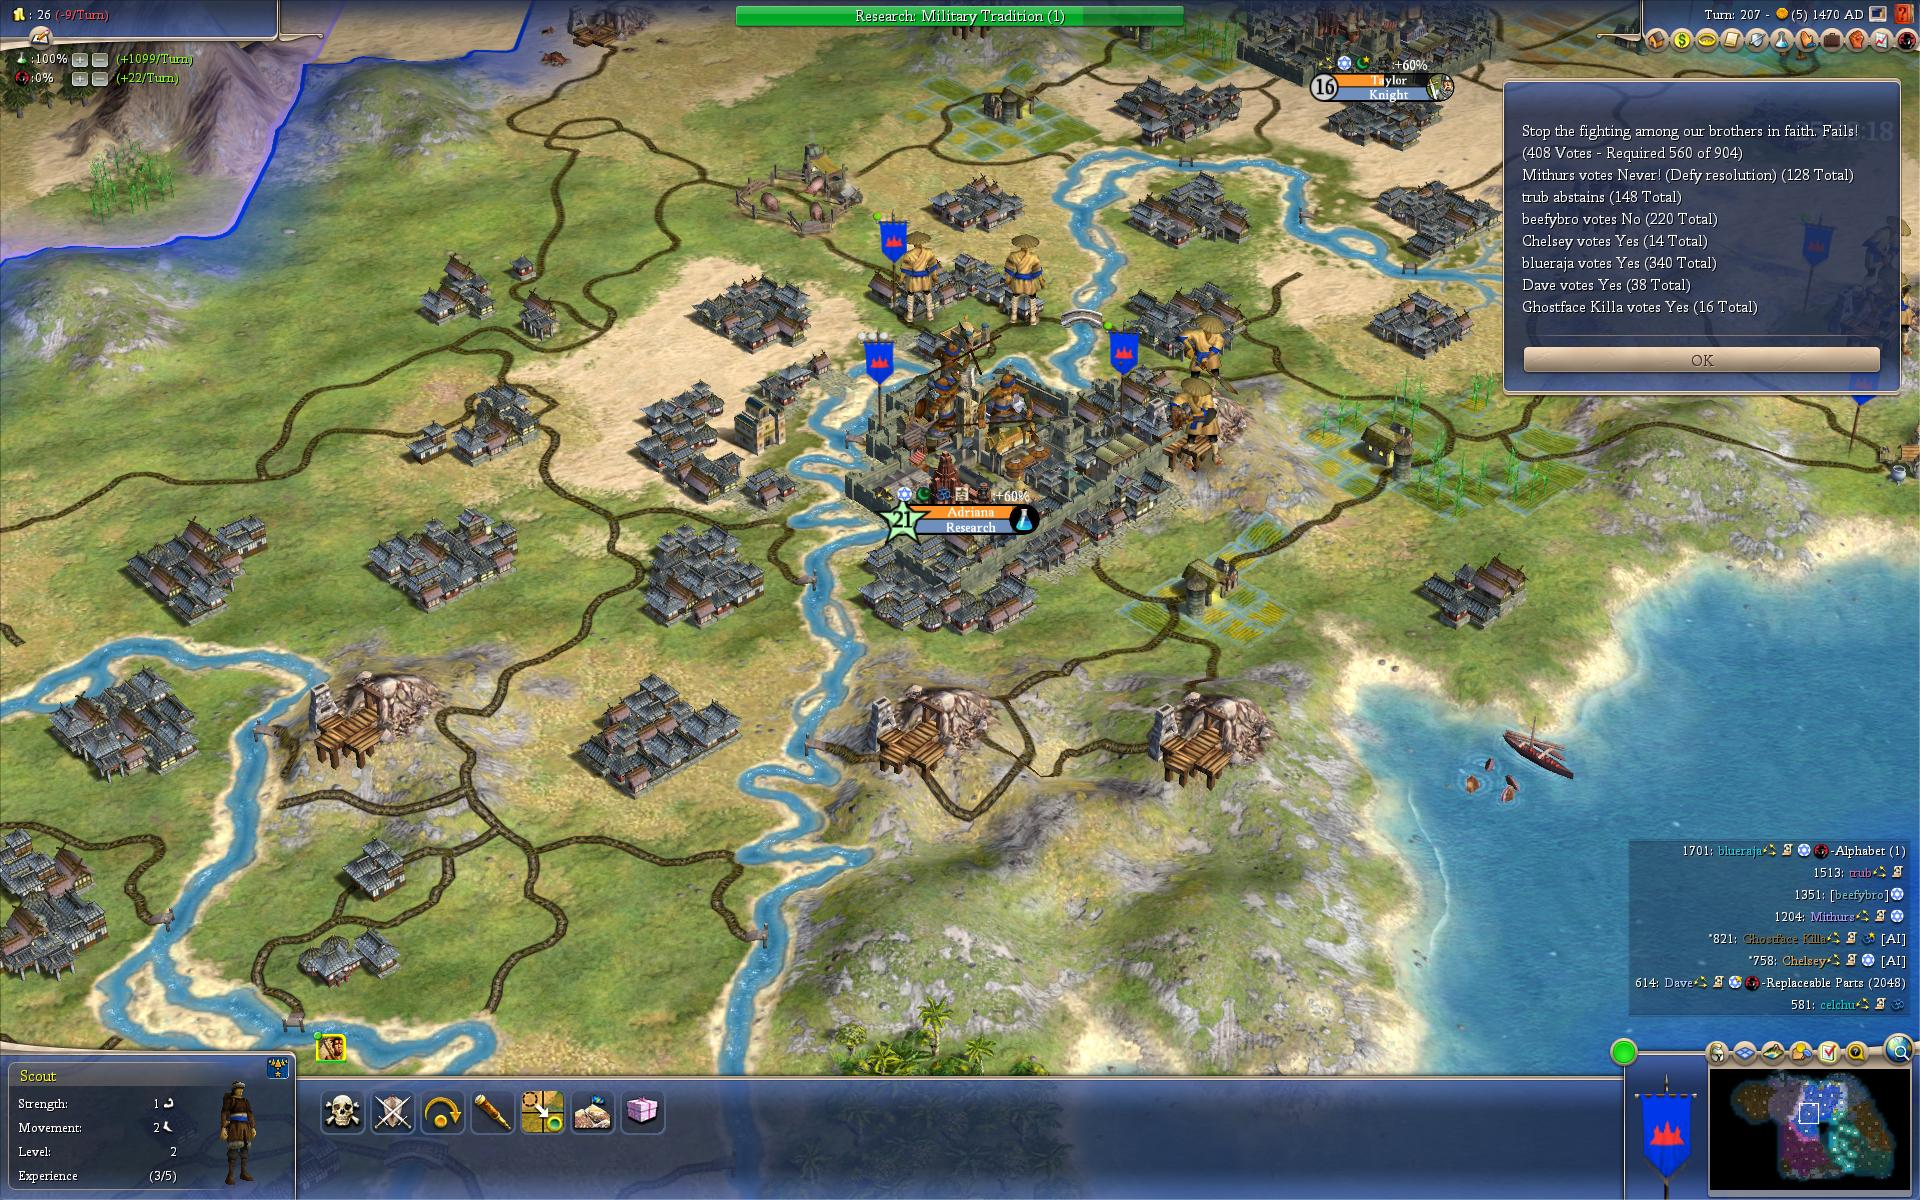
\includegraphics[width=1.0\textwidth]{turn207}

Thanks to Cop's abstain, we were able to block the stop-the-war
vote so Drew can continue his campaign.

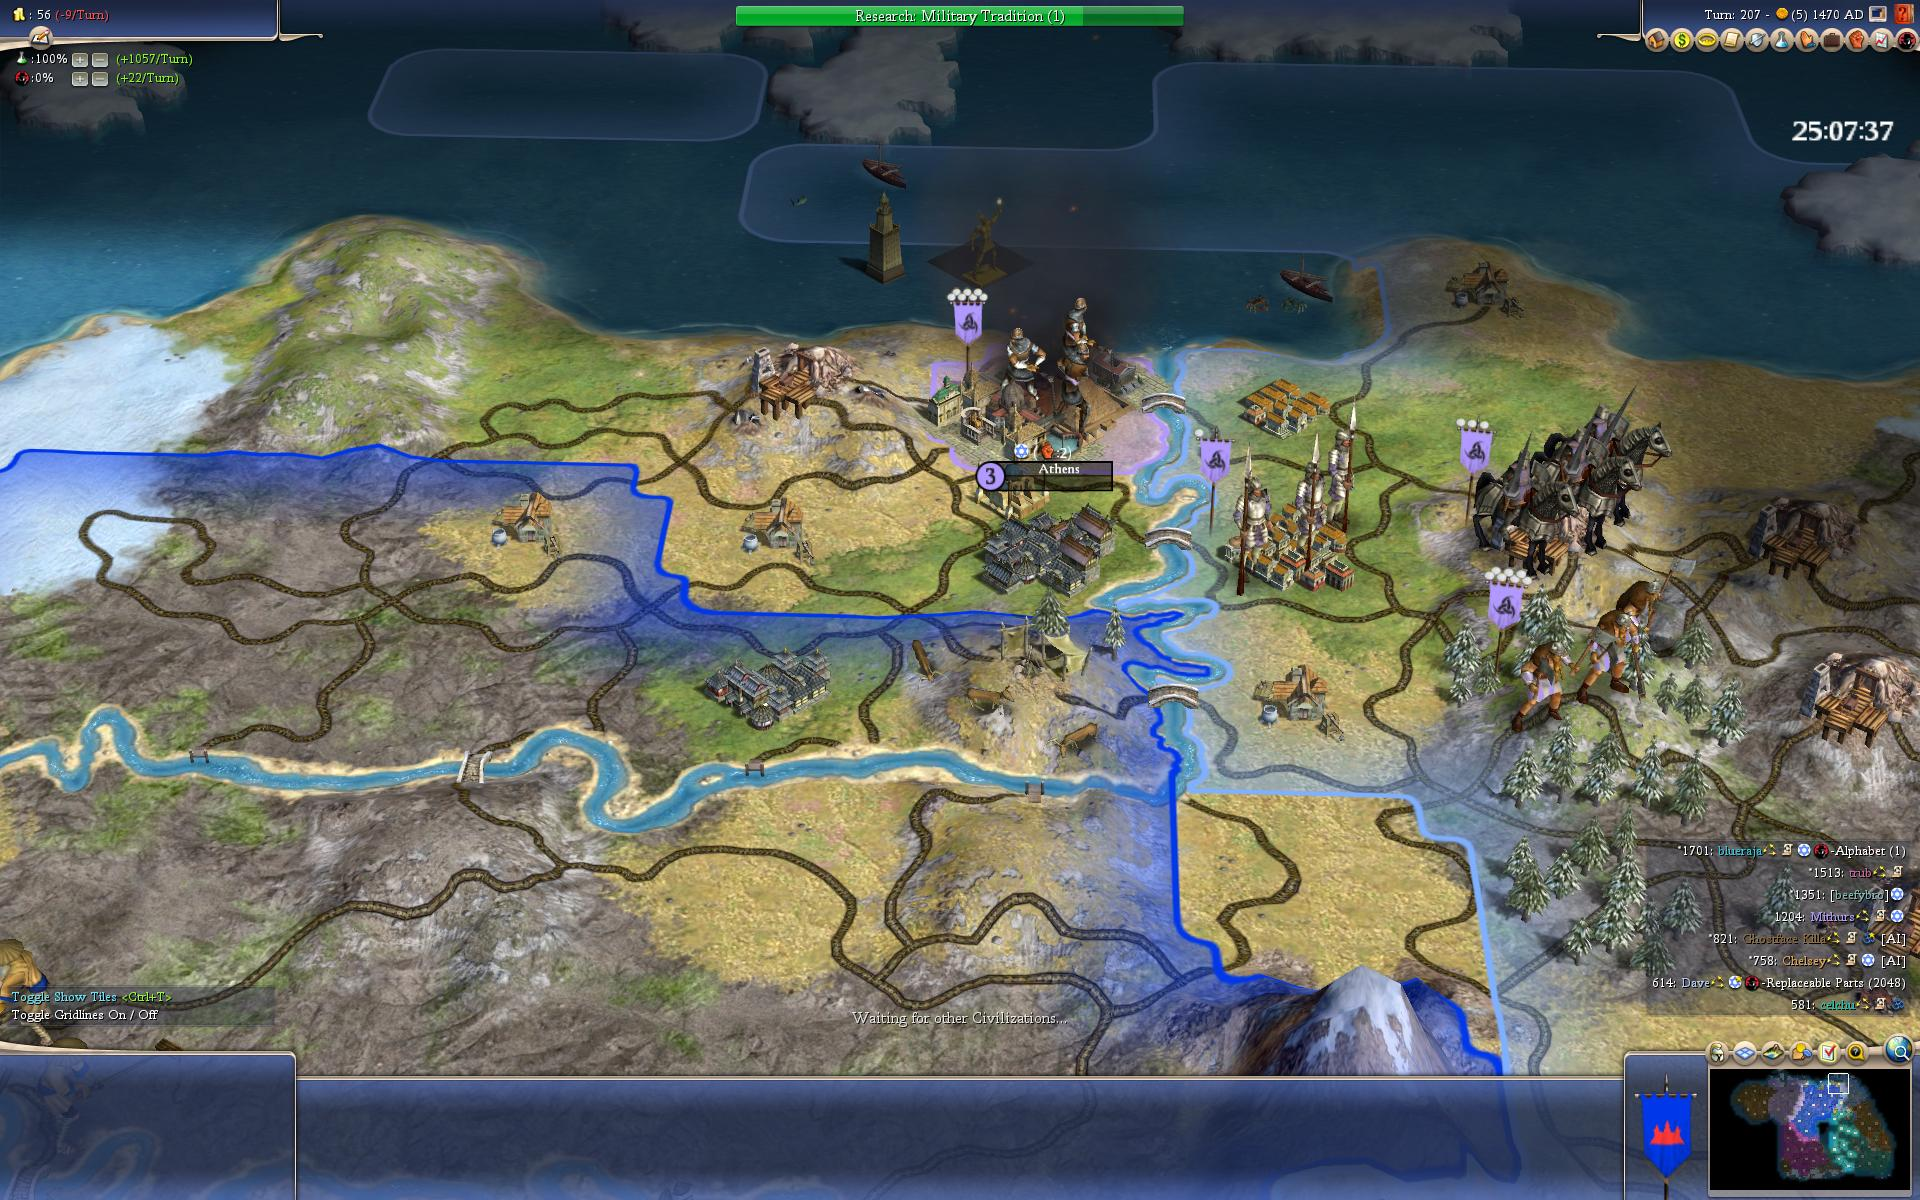
\includegraphics[width=1.0\textwidth]{turn207-2}

I made the very important decision to abandon the democracy beeline
and instead pick up the powerful mounted units of this era. Military
tradition, 3 turns of research, will give me curiessers and rifling (8
more turns) will give me calvalry. These are very powerful units that
have flanking attacks against cannon, so this will allow me to help
Drew in the case that Pat goes in against him. SoL will still be a
nice pickup, so that will come after rifles.

The other key choice is what to do with Jessica. I can either run a
huge number of specialists or pump more mediocre wonders. The wonders
will provide more specialists over the course of the game, but I could
use the great scientists now. My other 2 strong research cities need
academies. Another golden age would be very helpful as well. Probably
the highest priority wonder is the one that allows all religious
civics. This would allow me to switch to pasifism during my next age
to accrue massive GPP during the age. I'd probably switch back to
Theocracy or Organized Religion after the age.''

DaveCop cannot close borders with Pat due to the terms of his NAP, so that eliminates the trade embargo idea.

Demographically, my GNP is listed as significantly higher than Pat's,
but he seems to be researching techs significantly faster. It took him
just 3 turns to get steel; it's taking me that long to get techs much
farther back in the tech tree. Speaking of Pat's techs, he choose
military science (grenadiers) after steel which I find to be a very
strange choice. I'm not really sure why he'd go for grenadiers before
anyone, including himself, has rifles.

\section*{Turn 210}

The war between Drew and Karmol has turned into a full-blown proxy war
between Pat and myself with Pat feeding Karmol loads of cannons and me
feed drew fresh supplies of cuirrisiers. This event is becoming more
costly than I would have liked, but it has to be won or else Pat
wins. The plan is to beeline rifling, then run 0\% science to help
Drew upgrade all his units. That should give him the firepower to take
out Karmol barring Pat joining in more actively. After rifling,
probably the best idea is steel for cannons.

There is a potential role for Max in all this... if he runs 100\%
espionage and produces nothing but spies in all his cities, he could
do serious damage to Pat by knocking down towns in his capital
BFC. I'm not sure exactly how to convince him to do this without
breaking the spirit of our rules (every player should be trying to win
at all times). Running 100\% espionage is not something you'd do if
you were trying to win; not that Max has any real chance to win
anyway. I think this action could be justified in the context of
stopping a runaway.

According to Drew, DaveCop's attack against Mongolia got wiped. This doesn't bode well for having him help against Pat.

\section*{Turn 211}

Drew's stack of 50 units has been wiped out by a seige attack of a
dozen cannons followed up by knights, muskets, and older units. Lesson
learned: run from cannons! Lesson 2: always retreat if there's a risk
of getting wiped.

\section*{Turn 212}

Still digesting the consequences of what happened last turn. Drew has
a good plan: starve/whip Karmol's capital down to size 1 so that it
gets razed when it's recaptured; pretty devious! This would eliminate
the AP from the game. The plan is to be ready with a settler and some
rifles/calvary to take the spot that the cap is occupying. This could
mean war with Karmol, but my superior units should be able to keep the
city.

An even more daring plan is emerging: I should be able to beat Pat to
astronomy, opening up a potential sea attack on a couple good cities
of his. If I loaded a boat with 4 rifles, could it raze a coastal city
of Pat's?

Another nice thing would be to discover that the world is round.

Drew's last stand:

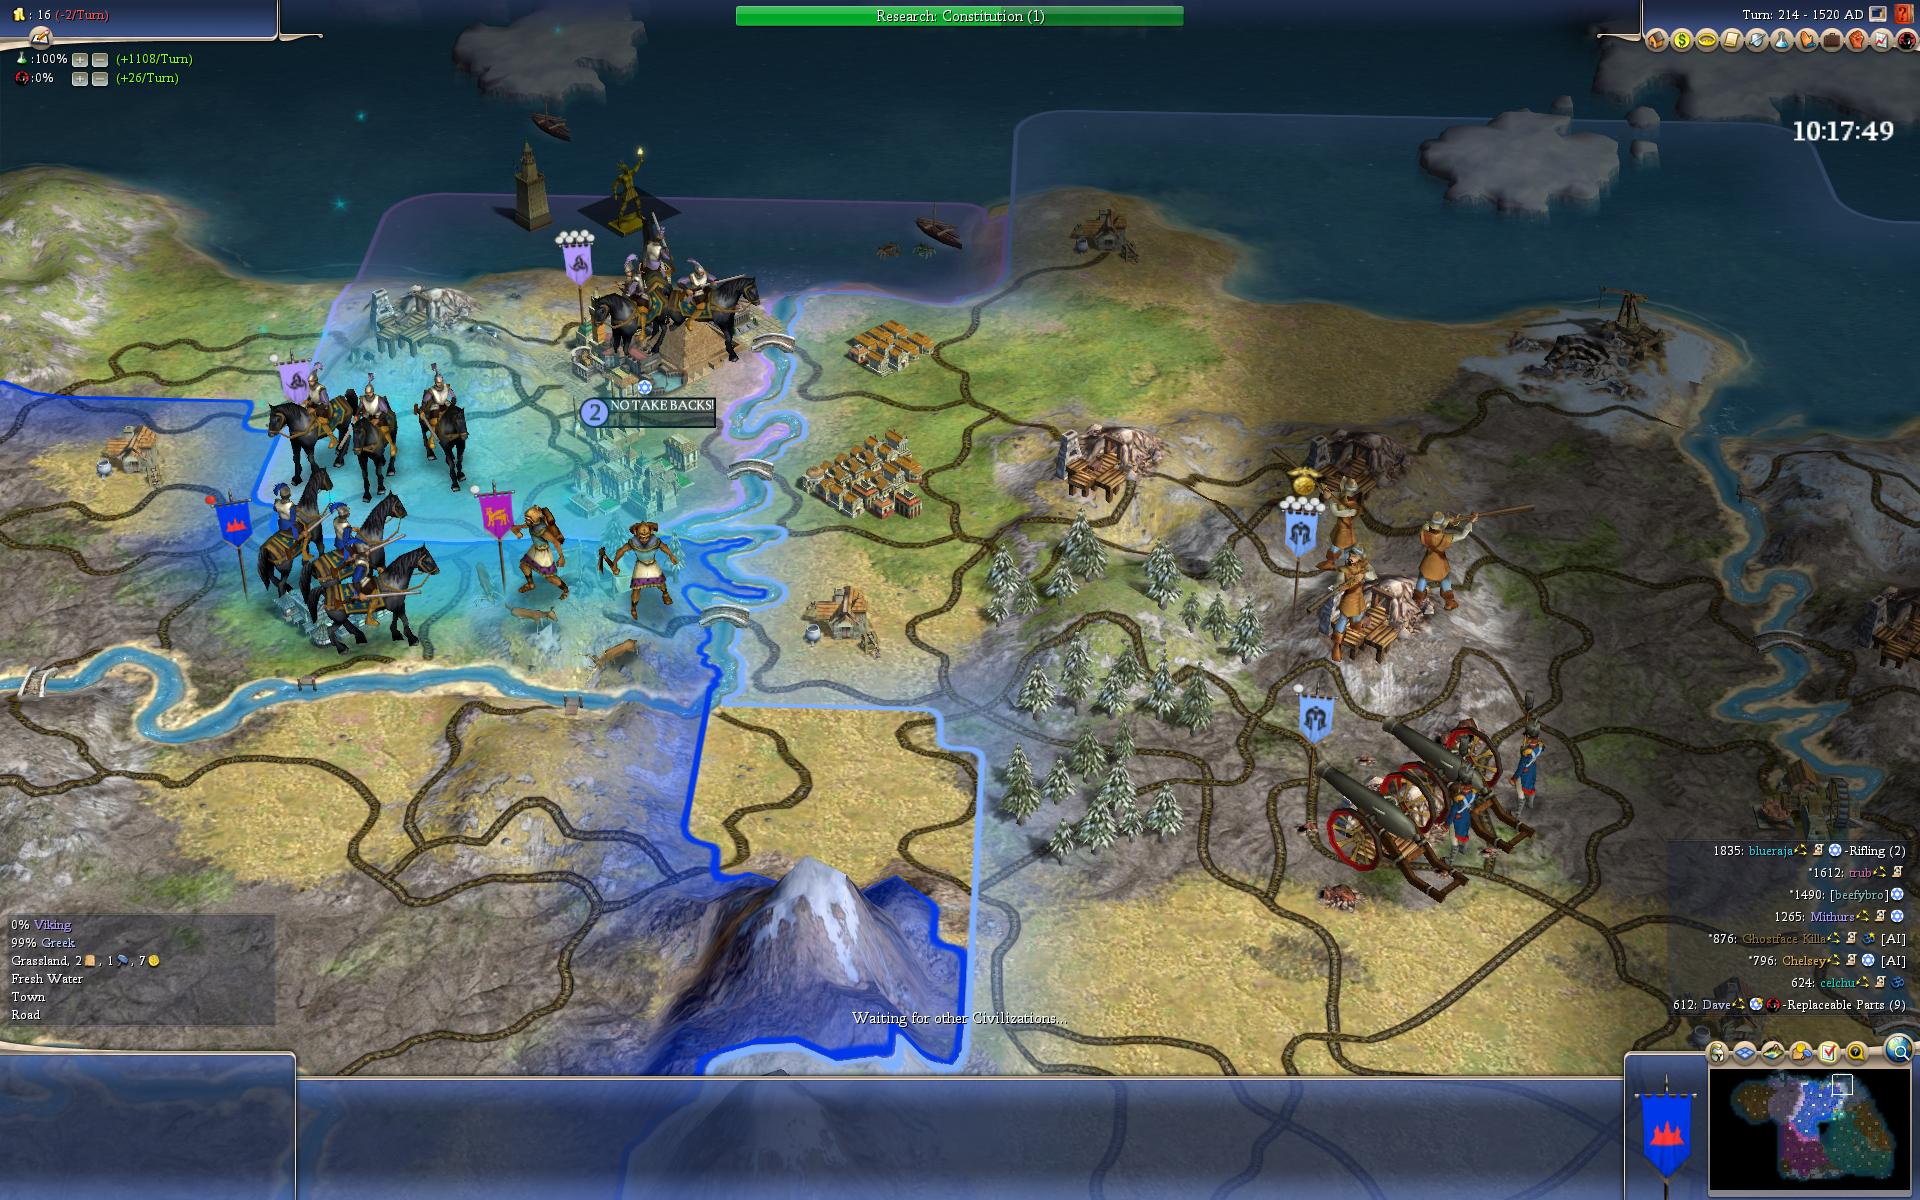
\includegraphics[width=1.0\textwidth]{turn214}

\section*{Turn 215}

Karmol has recaptured all the land drew took from him. This is a big
setback in the quest to knock Pat down a notch or two, but Karmol is
in bad shape at least and should make for an easy conquest with
infantry and cannon. Note that Karmol's capital was not razed since it
was a reconquest.

On the economic front, I've been doing a lot of thinking. For the time being, I need to optimize tech, which I think can be done as follows:
\begin{itemize}
\item Democracy -> Statue of Liberty
\item Switch to republic and pacifism: This will boost the value of the
scientist specialists provided by the SoL. Pacism will increase the GP
generated by Jessica; note that Jessica should not be the one to build
the SoL, it should just focus on producing great people instead. With
the SoL and pacifism, Jessica should be a monster GP city. The switch
to these better civics should be done as soon as philosophy is
complete unless Pat appears to be going for SoL as well. At a later
point, the switch should be made to free market during a GA. Switching
to free religion is tempting; perhaps this should be done after I milk
pacifism for a while.
\end{itemize}

\section*{Turn 221}

Pat looks to be going for SoL as well; fortunately, I got a
game-changing random-event: free great artist! Jessica will produce a
great scientist (probably) in 4 turns, so that would give me a
golden-age switch to democracy, turning my capital into a production
giant to finish off the SoL. A later switch will need to be made to
pacifism and representation. I'm going for economics and coporation
for a free switch to free market and adding an additional trade route
in all cities.

The game seems to be taking a turn towards espionage being much more
of a factor. Pat is investing in it heavily and he recently lost a spy
in my territory. I think he could be trying to sabotage production of
the SoL, so I need to at least have a defensive spy in the capital and
a counter-espionage mission on pat.

\section*{Turn 222}

Pat has declared on Sitting Bull who only has longbows to defend his
cities, so he's going to gobble him up fast. This puts pressure on me
to do something, probably attack Karmol as soon as his session as pope
is done.

The NAP with DaveCop is over in 18 turns.

\section*{Turn 226}

Sitting Bull is losing cities fast. Fortunately, Karmol got the jewel of the bunch, SB's capital.

I've popped my golden age and switched to free market and democracy, making my demographics look good:

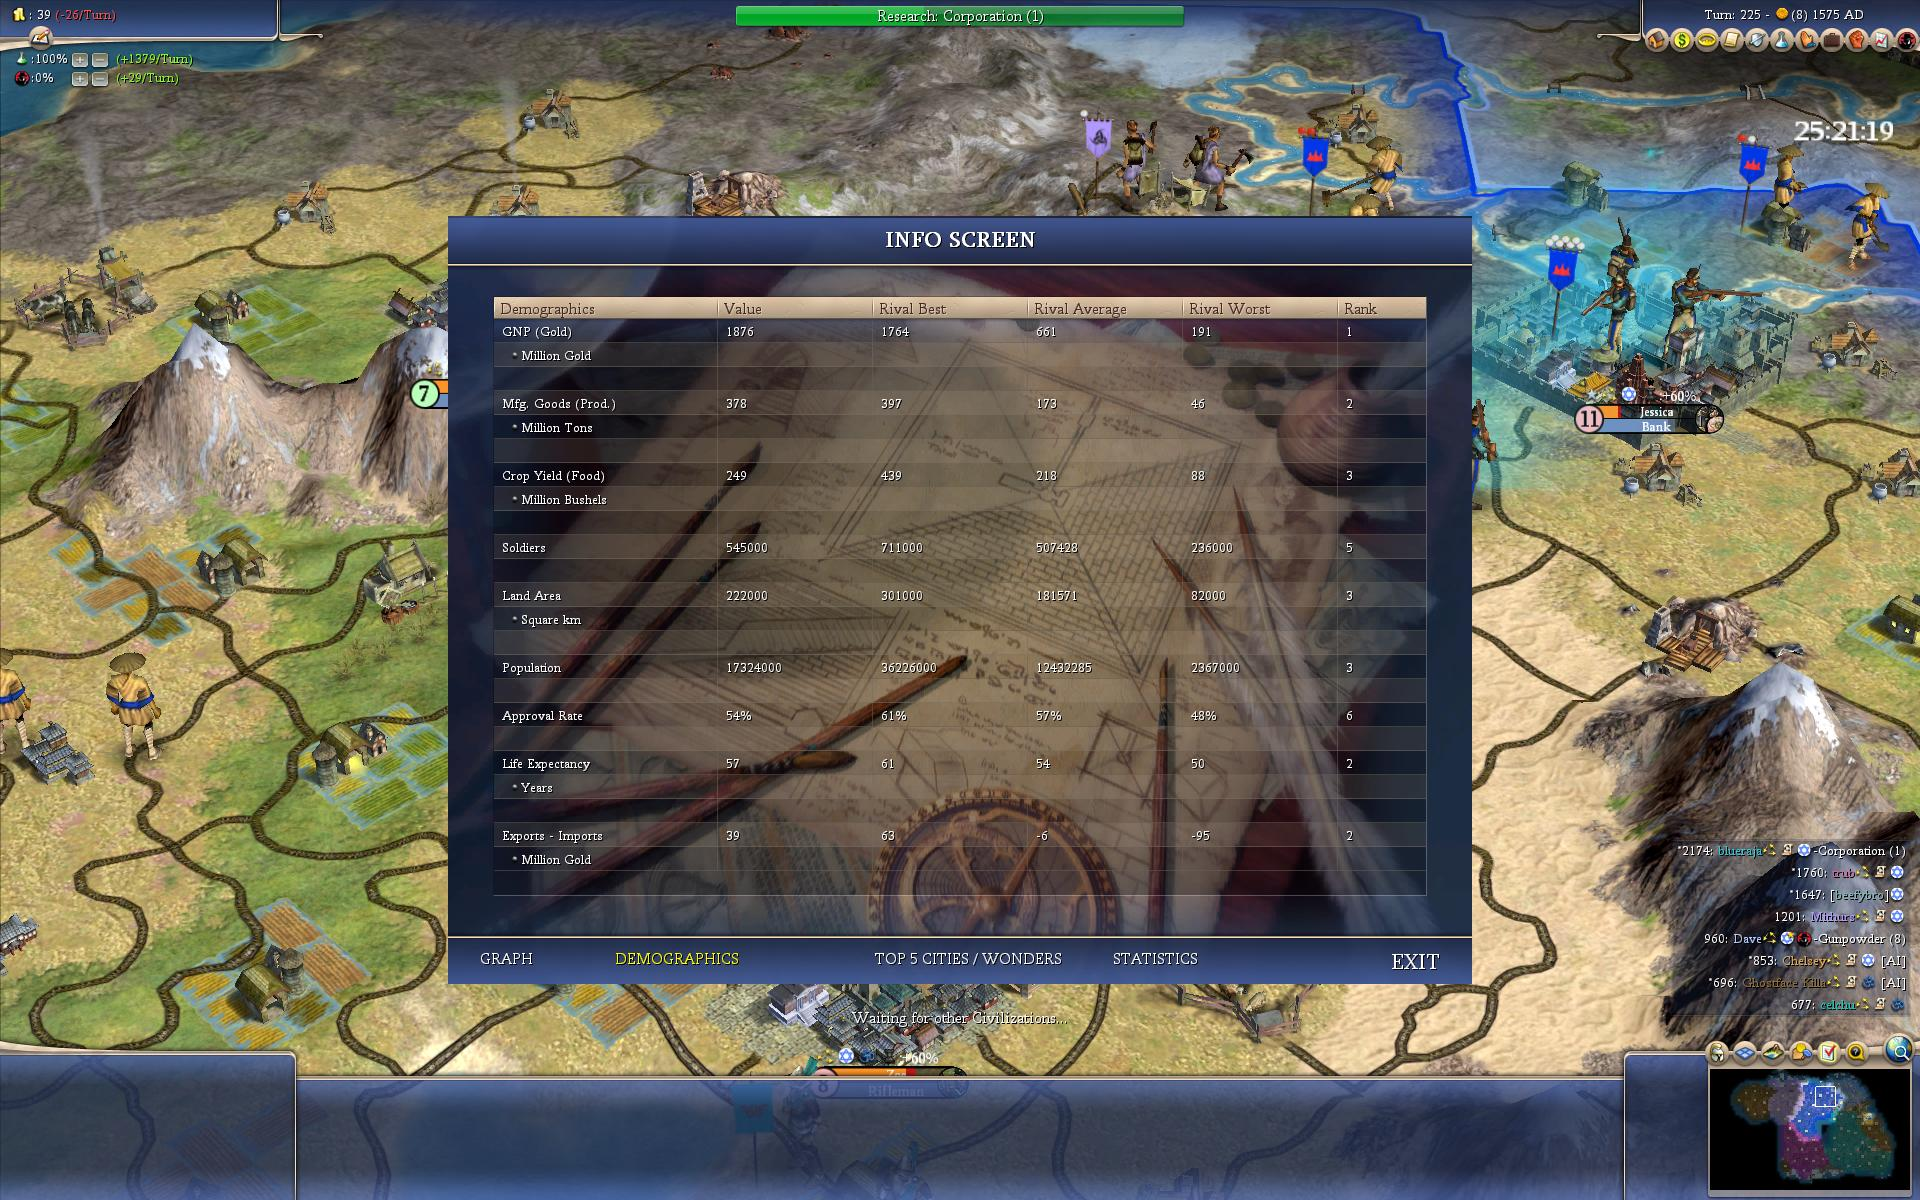
\includegraphics[width=1.0\textwidth]{turn225}

Evidence is mounting that Kuan is acting as a double-agent! Pat seems
to be aware of civ issues that Drew and I talked about on the ski trip
in front of Kuan.

Some doubts are in my mind regarding pacifism and especially representation. This is the optimal civic combo with the SoL to maximize GNP, but at a significant cost in my production capabilities. Assuming I ran all scientists:
(9 cities + 6 extra scientists) * 3 extra science per city * 1.7 average sci bonus = ~76 science not including civ-wide bonuses like researching techs that are already known or research techs for which extra prereqs are known. Let's say the end result could be around 100. This comes at a cost of
25 towns * 2 average bonus = 50 hammers
On the other hand, representation also comes with a nice happiness bonus.

Theocracy or Pacifism could be better than OR. Pacifism is 0 upkeep,
which is excellent compared to high-upkeep OR. I could potentially
pump great merchants from Jessica to power my economy.

\section*{Turn 227}

New election for pope... Karmol won againl; I abstained out of spite:

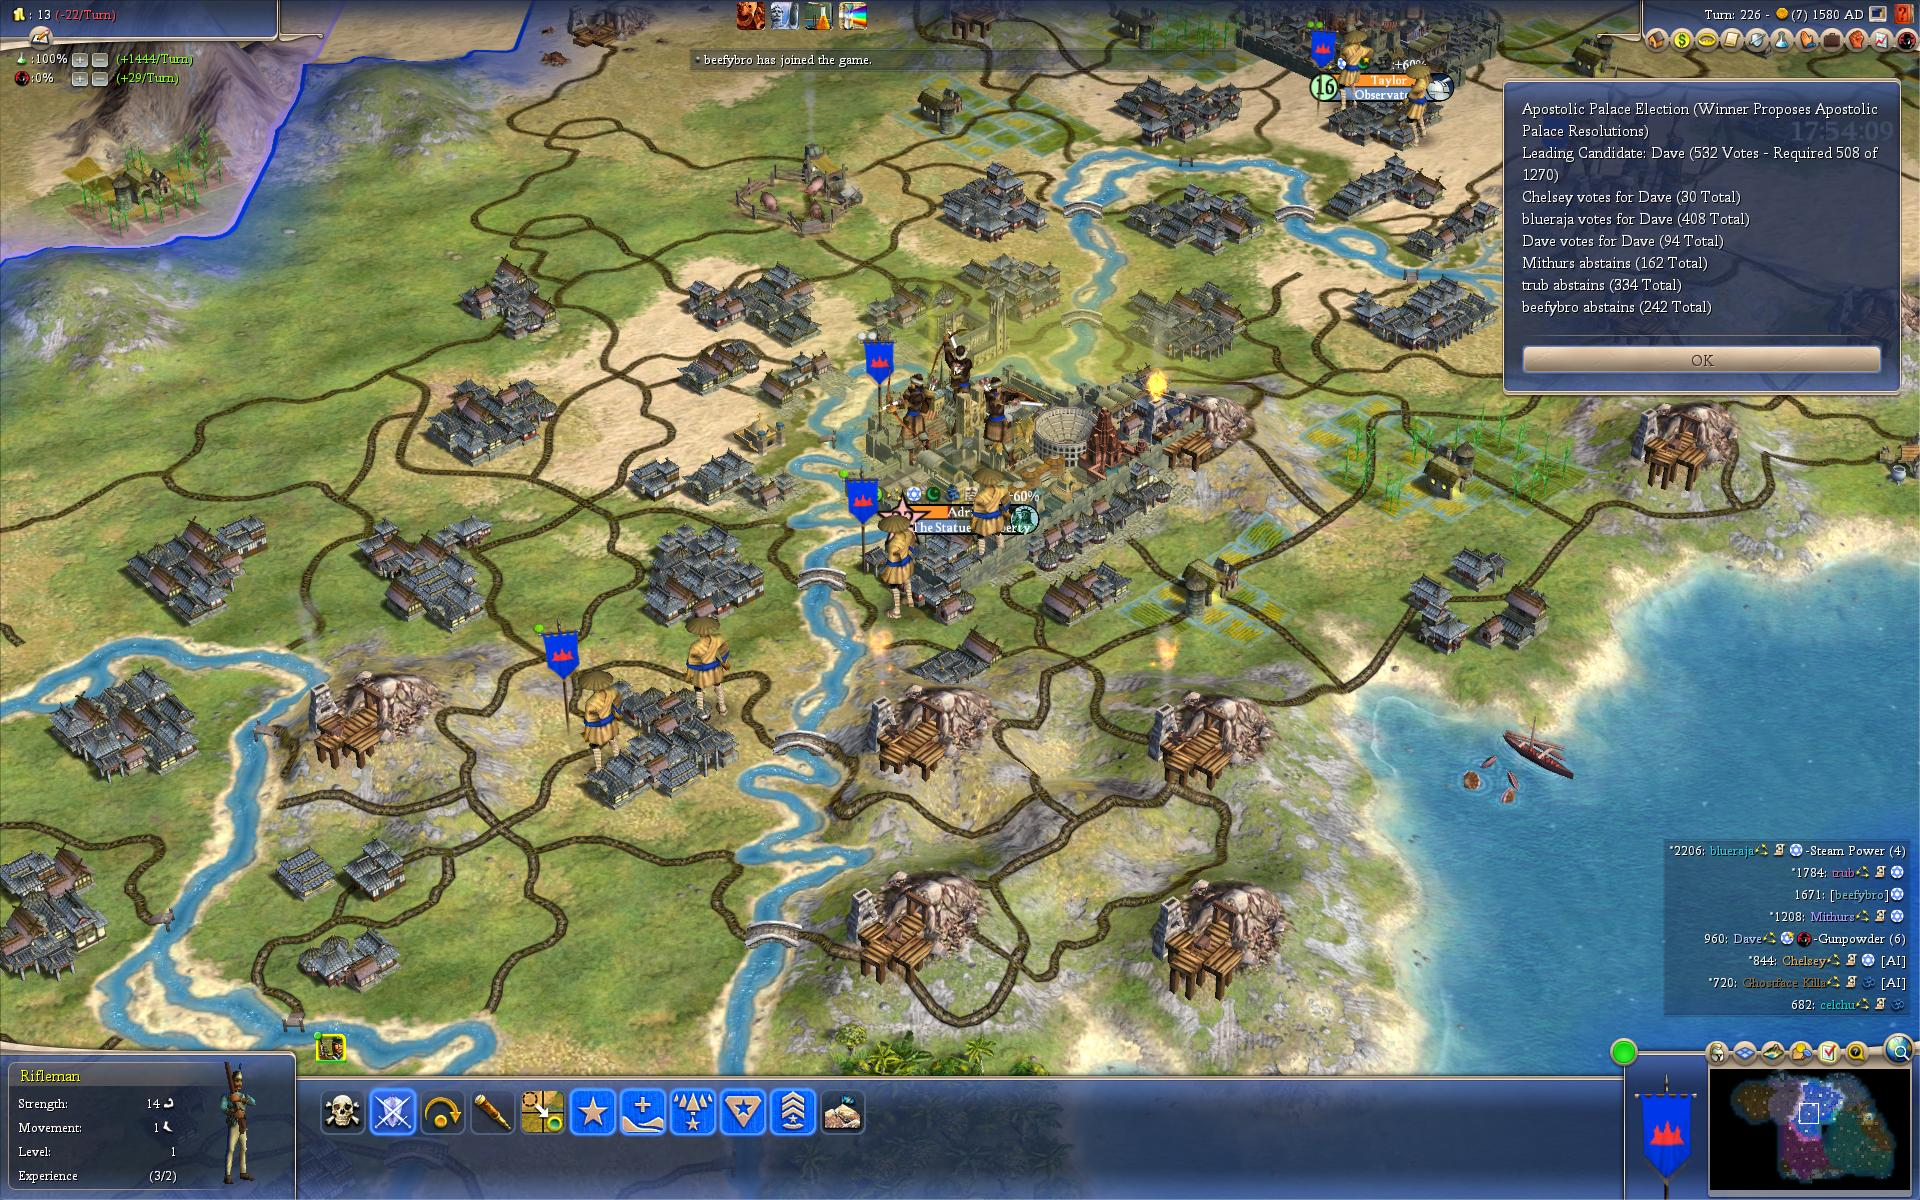
\includegraphics[width=1.0\textwidth]{turn226}

I've informed Pat that the deal with Karmol is over. Karmol has some
lightly defended cities near me that I'm tempted to take. I have to at
least take Tokyo or else I won't be able to walk to Pat by land.

Pat is not having any trouble keeping up with me in GNP. Trying to outtech him is a long-lost cause.

I've sent the following email to Cop, Drew, and Max to try to coordinate the actions against Pat:

"""
Hi Guys,

I was wondering if we could meet on steam sometime soon (tonight or this weekend) to coordinate an attack on Pat. I've been burning a lot of neural cycles thinking about this and I think I have a plan.

Here are facts and/or things I think we can agree on:
\begin{itemize}
\item Pat is running away with the game
\item None of us is in a position to single-handedly do much damage to him
\item Pat's NAP with Cop expires soon (15 turns I think)
\item Once infantry is available there is a window where no better units are available for a while (artillery and tanks are a ways off).
\end{itemize}

Here's the plan:
\begin{itemize}
\item Cop and I beeline up to infantry, cannons, machine gunners
\item Cop and I mass-upgrade all our units
\item Cop does an all-out attack on Pat's SW territory on the same turn as his NAP runs out
\item On that same turn, I do an all-out attack on Pat's NW territory
\item A few turns later, I do a fake sea invasion to try to pull some units away from the front
\item Once Pat's army is preoccupied with Cop and I, Max begins his espionage assault on Pat. Since Pat is running Democracy, I think the best thing to do is to focus on sabotaging his towns down to cottages.
\item Drew is not in a position to help directly since he's too far behind in tech, but he can help by contributing gold, resources, and gift old units to be upgraded. The exact details of this need to be worked out.
\end{itemize}

Thoughts?

-Jim
"""

\section*{Turn 228}

Karmol is still several turns from gunpowder and would be extremely easy to wipe out if I didn't have to worry about Pat. I'm almost tempted to tell Pat that the pile is coming but I will hold it off if he allows me to gobble up Karmol.

\section*{Turn 230}

I've decided to go ahead with the deal with Pat. He's teching too fast
and has too much unit-producing potential with massive raw production,
drafting, and whipping; I think the odds of a military victory are
low.

Here's the case as I laid it out for Pat:
\begin{itemize}
\item there are no good wonders in any of the land in question
\item i would still be smaller in pop and production compared to you
\item If you remain in first place by 600 points or w/e, you're going to get piled
\item piles can be pretty unpleasant even if the military situation is a stalemate
 such as: loosing all foreign trade routes, being forced to draft/whip/making nothing but military, hostile espionage
\item the Karmol is alliance is not worth much to you
\item I'm willing to offer a wide range of NAP, trading deals
\end{itemize}

In return, I'm asking for full annexation of Karmol without Pat interviening. We'll see if he accepts.

\section*{Turns 231-248}

Pat accepted the deal on the condition that I only get 4 key cities of
Karmol's. I also helped work out a deal so that DaveCop was not left
out to dry in this deal; Pat will gift him 80g/turn for 30
turns. Here's the deal in it's entirety:

The Jessica Convention v1.0, signed by all parties in 1620 AD

"""
Maya offers:

    NOT to give units to or upgrade the units of Greece while it is being attacked by Khmer
    80 gold per turn to Babylon for 30 turns
    50 turn NAP to Khmer
    30 turn NAP to Babylon
    50 turn NAP to Korea
    50 turn NAP to Vikings


Khmer offers:

    50 turn NAP to Maya
    to take ONLY the cities of Athens, Sparta, Corinth, and Tokyo from Greece.  Other Grecian cities will not be attacked.


Babylon offers:

    30 turn NAP to Maya


Korea offers:

    50 turn NAP to Maya


Vikings offer:

    50 turn NAP to Maya
"""

DaveCop is not entirely happy with this deal, which is
understandable. But this deal is much lower risk and improves the
geopolitical situation for both he and I (but more so for me). With
these cities of Karmol's I can serve as a counterbalance to Pat,
helping to keep him in check.

\section*{Later}

Karmol is strangely leaving most of his forces in the far east in
Brad's old territory and I've been taking his western cities easily.

\section*{Later}

Betrayal! Pat has broken our NAP and routed my forces in Toyko, losing
6 cannons or so to kill 20-some units. It is disappointing that Pat is
stooping this low despite already being in awesome position to
win. Rubbing salt in the wound, he explained that he was enforcing my
ancient NAP with Karmol, even though we just spent the last week
negotiating which cities of Karmols I was going to take... In any
event, my chances of winning this game have now dwindled to near zero;
I'm switching to nationhood, slavery, and theocracy to make a final
stand and do as much damage to Pat as possible. All remaining forces
in Karmol's land need to retreat back to Jessica to save that city
from Pat. If Pat gets the Minaret and Sankore, the game is so over.

\section*{Later}

All cities outside the core commerce cities are being drafted and they
are shrinking fast. Pat looks like he is, in fact, going to make an
attempt on Jessica. He's moving a large ~40 unit stack towards it and
I have trebs and a few infrantry and calvary defending. I've asked
Drew for a war loan of 500g to upgrade the trebs to cannons and he's
agreed. I need to pay him back 600g in 10 turns or so. Karmol has
taken back all his cities.

\section*{Later}

Victory! I hit Pat's stack with cannons followed by calvary. The
cannons were not particularly effective due to Pat having lots of
units immune to collateral damage (cannons and machine gunners), but
it was enough. I followed up with the calvary and they were quite
successful, getting several kills and nailing cannons with flanking
damage. Pat foolishly left the surivivors near Jessica, even
sacraficing a few cannons into the city defenders. With flanking
damage actually killing lots of cannons, the rest of the stack was
mopped-up. This was a great example of how powerful mounted units can
be, they were able to quickly retreat out of Karmol's land and get to
where they needed to be and did tons of damage when they got there,
this lesson should not be forgotten. The final tally was 15 losses on
my side to kill 39 on Pat's side.

\section*{Later}

With Pat's defeat at Jessica, the top priority is taking Athens back;
it has the statue of Zeus in it, and if I'm able to get it, Pat will
suffer serious war weariness due to all the losses he's taken. Karmol
has a lot of units defending, but most are medieval age. The cannons
are the main concern.

DaveCop is hesitant to help me against Pat since he feels kinda burned
by my decision to abort the pile. Now Pat is in another long
golden-age and things are incredibly dire; hopefully I can convince
him to help. Hindsight has revealed that aborting the pile was a huge
mistake on my part.

\section*{Later}

Defeat! Turns out, Karmol had enough to wipe my 15 atacking units,
although he took heavy losses (22) to do so. It shouldn't be too hard
to finish him off, but Pat is quickly rebuilding his nearby
forces. All my non-core cities are drafted down to below 7 pop and can
no longer be drafted, so I've started drafting in core cities. This
effectively ends my game, but I don't really have any choice.

On a side note, spies reveal that Pat's coastal cities are virtually
undefended, with just 1 acher in each. I'm going to try to sneak a
couple infrantry onto a boat for an amphibious attack.

\section*{Later}

In what is probably my best moment of the game, I razed Pat's 2nd-best
city, his wonder city, with an amphibious attack, dropping his score
by over 200 points. DaveCop's score is now not too far behind Pat's,
although I still think Pat is way out in front.

\section*{Later}

I've hinted to Cop that I'm not long for this world and my defenses in
my cities near to him are light. At this point, I'm more than happy to
lose these cities to Cop if it helps to deny Pat the win. These are
the dangers of making a player really angry in civ! Pat was furious
about losing his wonder city and even admitted to yelling at his
family after he saw the damage. I think it's very safe to say we'll be
fighting until my last city is off the map.

\section*{Later}

Cop took the bait and has begun to annex all my land. I drafted and
whipped every last drop out of each city before he got it, sending it
all to Jessica to fight Pat. This seems to be working pretty well as
Pat and I are still stalemated in the Jessica region despite now the
now ridiculous advantages he has over me in the demographics.

\section*{Later}

Cop has nearly annexed my entire empire and Pat and I are *still*
fighting it out near Jessica. Pat was clearly deflated by the loss of
his best city and his attacks against me have not been as potent as I
had expected. I'm still sniping units here and there, doing damage but no
major wipes.

\section*{Later}

Amazingly, Copithorne was able to get all my cities, denying Jessica
to Pat! Cop's economy is really rolling now and I think the tables may
have turned for good. With Pentagon, theocracy, and aggressive, Cop's
units are coming fresh out of the barracks scary strong. In a cheesy
move, Drew has given me a "reservation" city light years away from Pat
in the tundra in order to preserve Pat's war weariness. Pretty devious
but I'm not sure how I'd feel if a player did this to me. If it
weren't for the flagrant NAP bust earlier, I might have gone out in
more sportsmanlike fashion... or not.

\section*{Recap}

Pat has conceded and the game is over! Not exactly a win from my point
of view but I can live with a Copiwin. Just out of curiousity, we ran
the game to end with AIs in control over all players; Copithorne bot
completely dominated. I think it's fair to say Cop's position at the
end of normal play was even more dominant than it appeared. It was
revealed that Cop had settled an Australia-sized continent just to the
SW of the main pangaea continent.

Couple lessons here: first, a furious player can have a massive impact
on the game even once they've been knocked out of contender
status. Pat surely would have coasted to victory if it were not for me
sacrificing my entire empire to hurt him as much as possible and help
his rival as much as possible. That leads in to second lesson: human
diplo skill is easily as important as civving skill. Copithorne is not
an experienced player and yet crushed everyone in the end. He was able
to lurk in the middle of the contender pack without any real setbacks
and then skyrocket right at the end. If memory serves, no human player
ever even declared on Cop!  How is it possible to win a game without
ever being declared on!? Epic diplo for sure. I think no one ever saw
him as a real threat until the end, combination of him being a newer
player and his civ being middle-of-the-pack for most of the game.

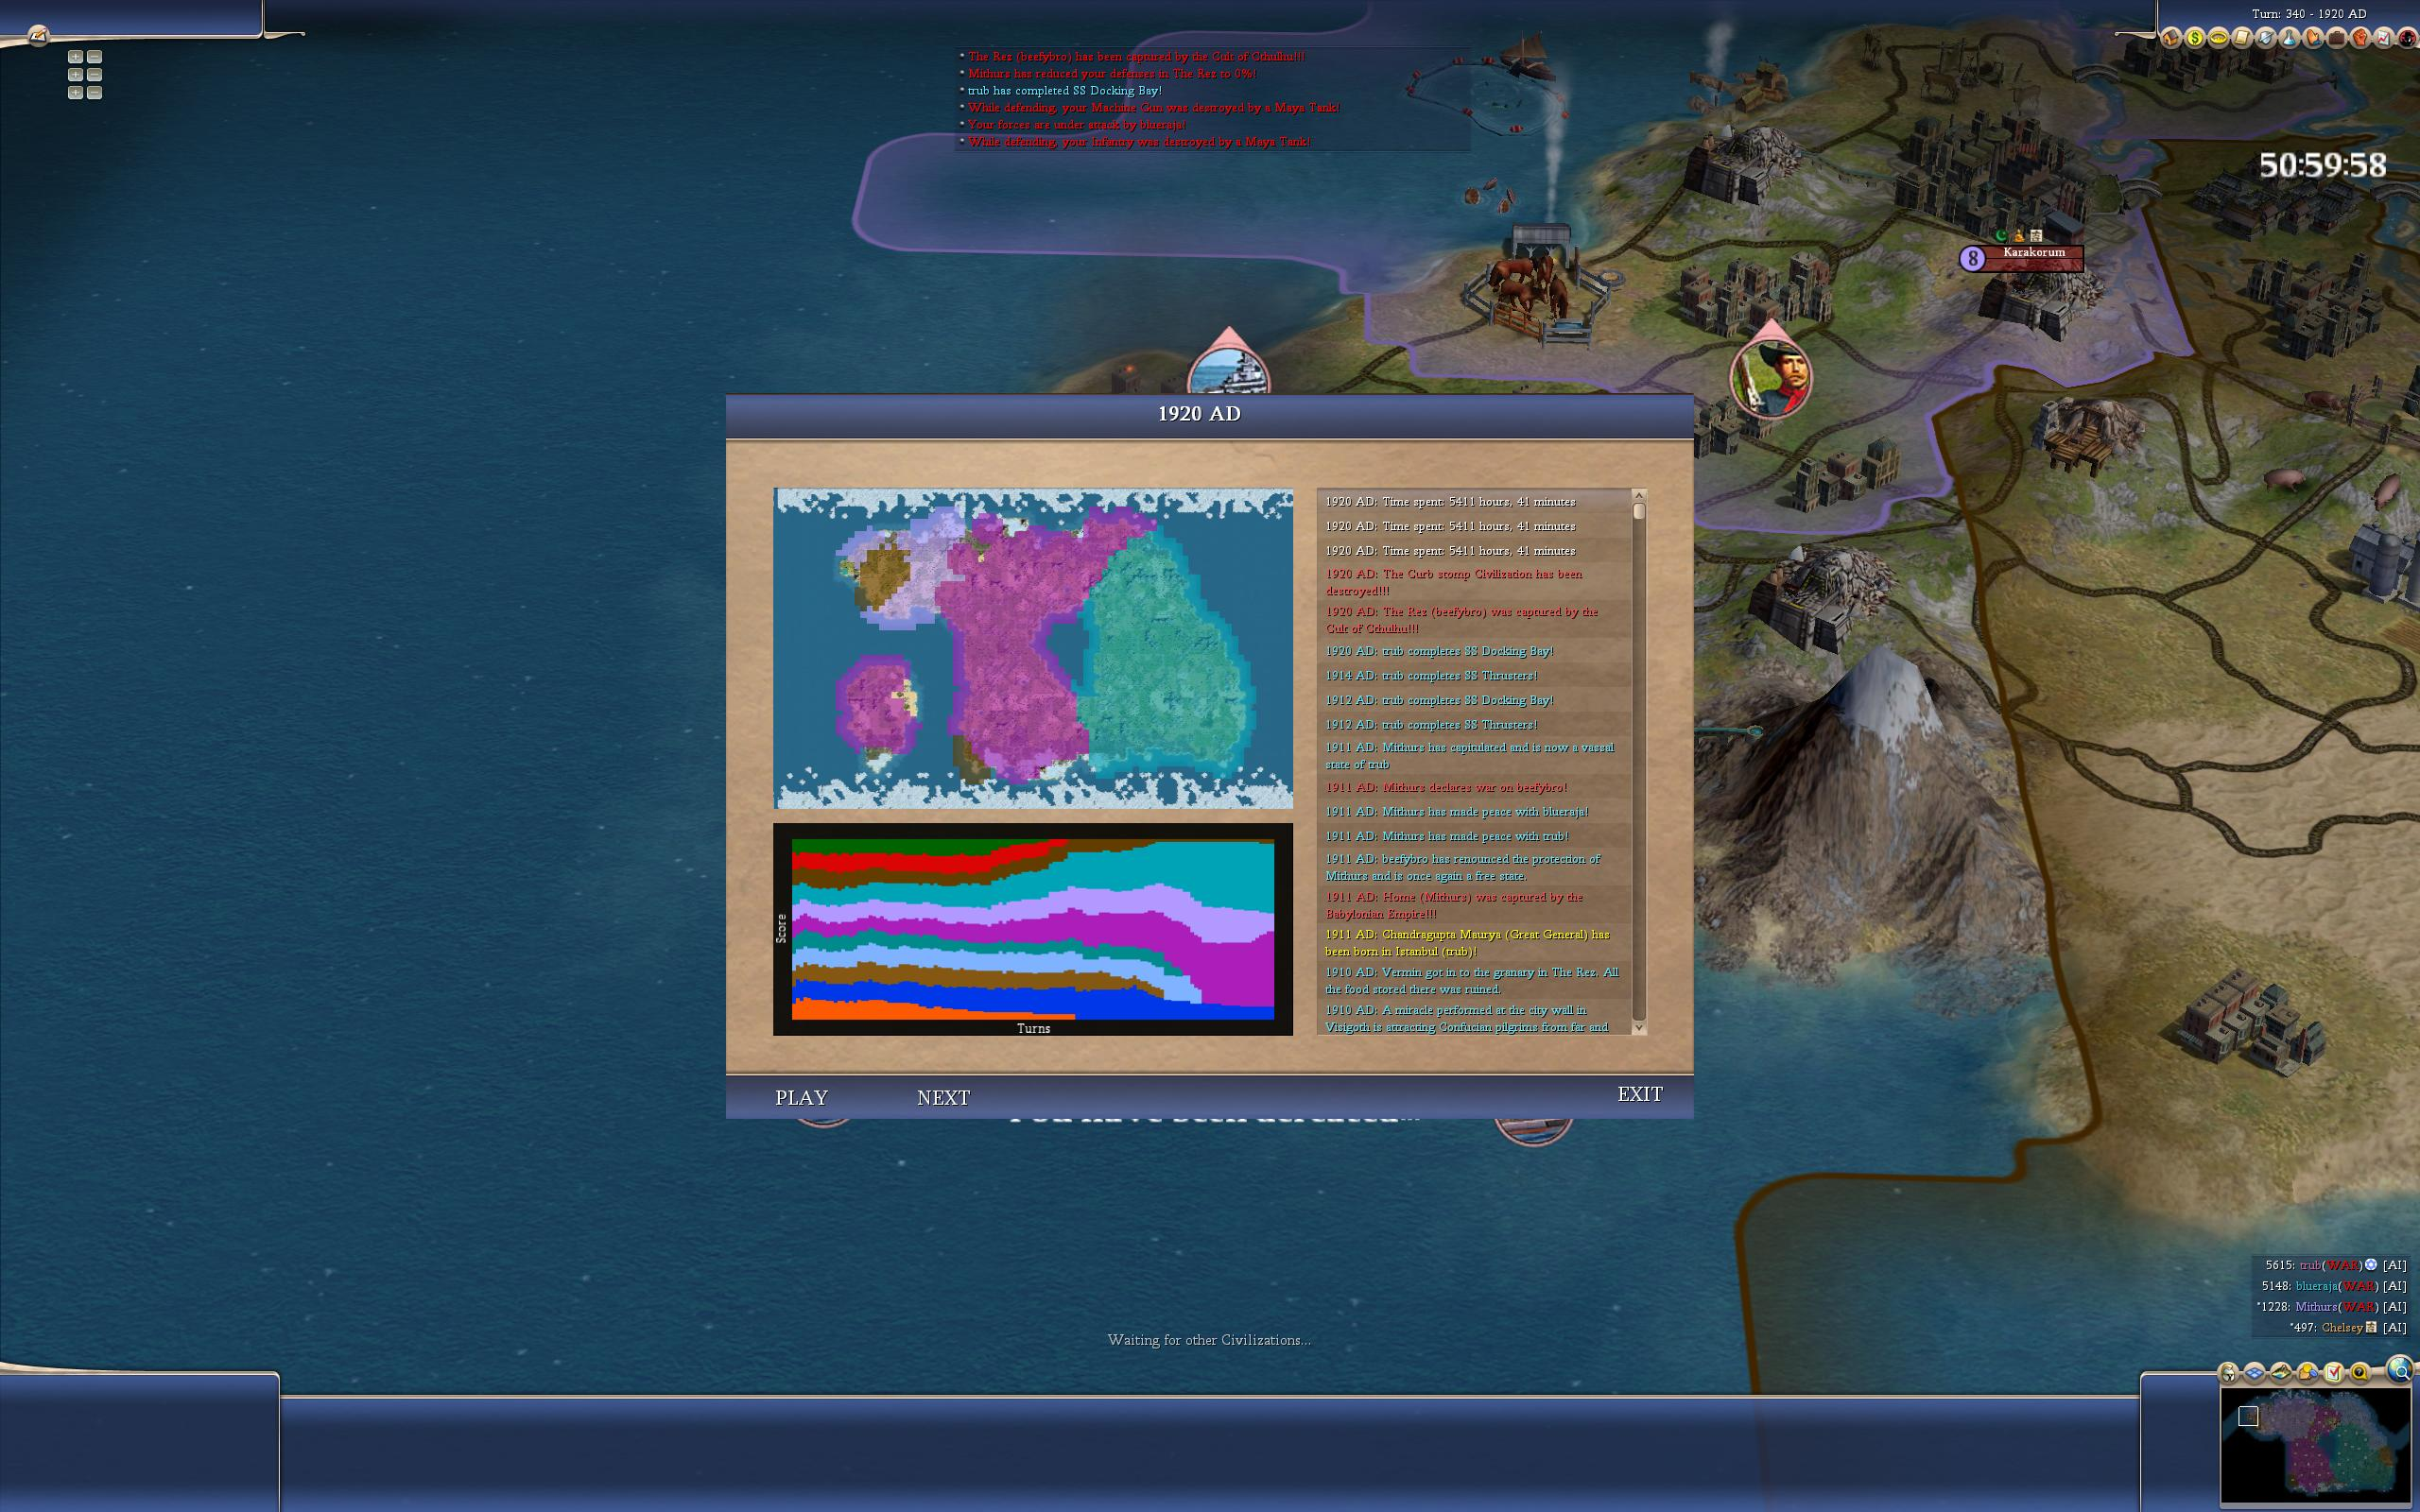
\includegraphics[width=1.0\textwidth]{end-1}
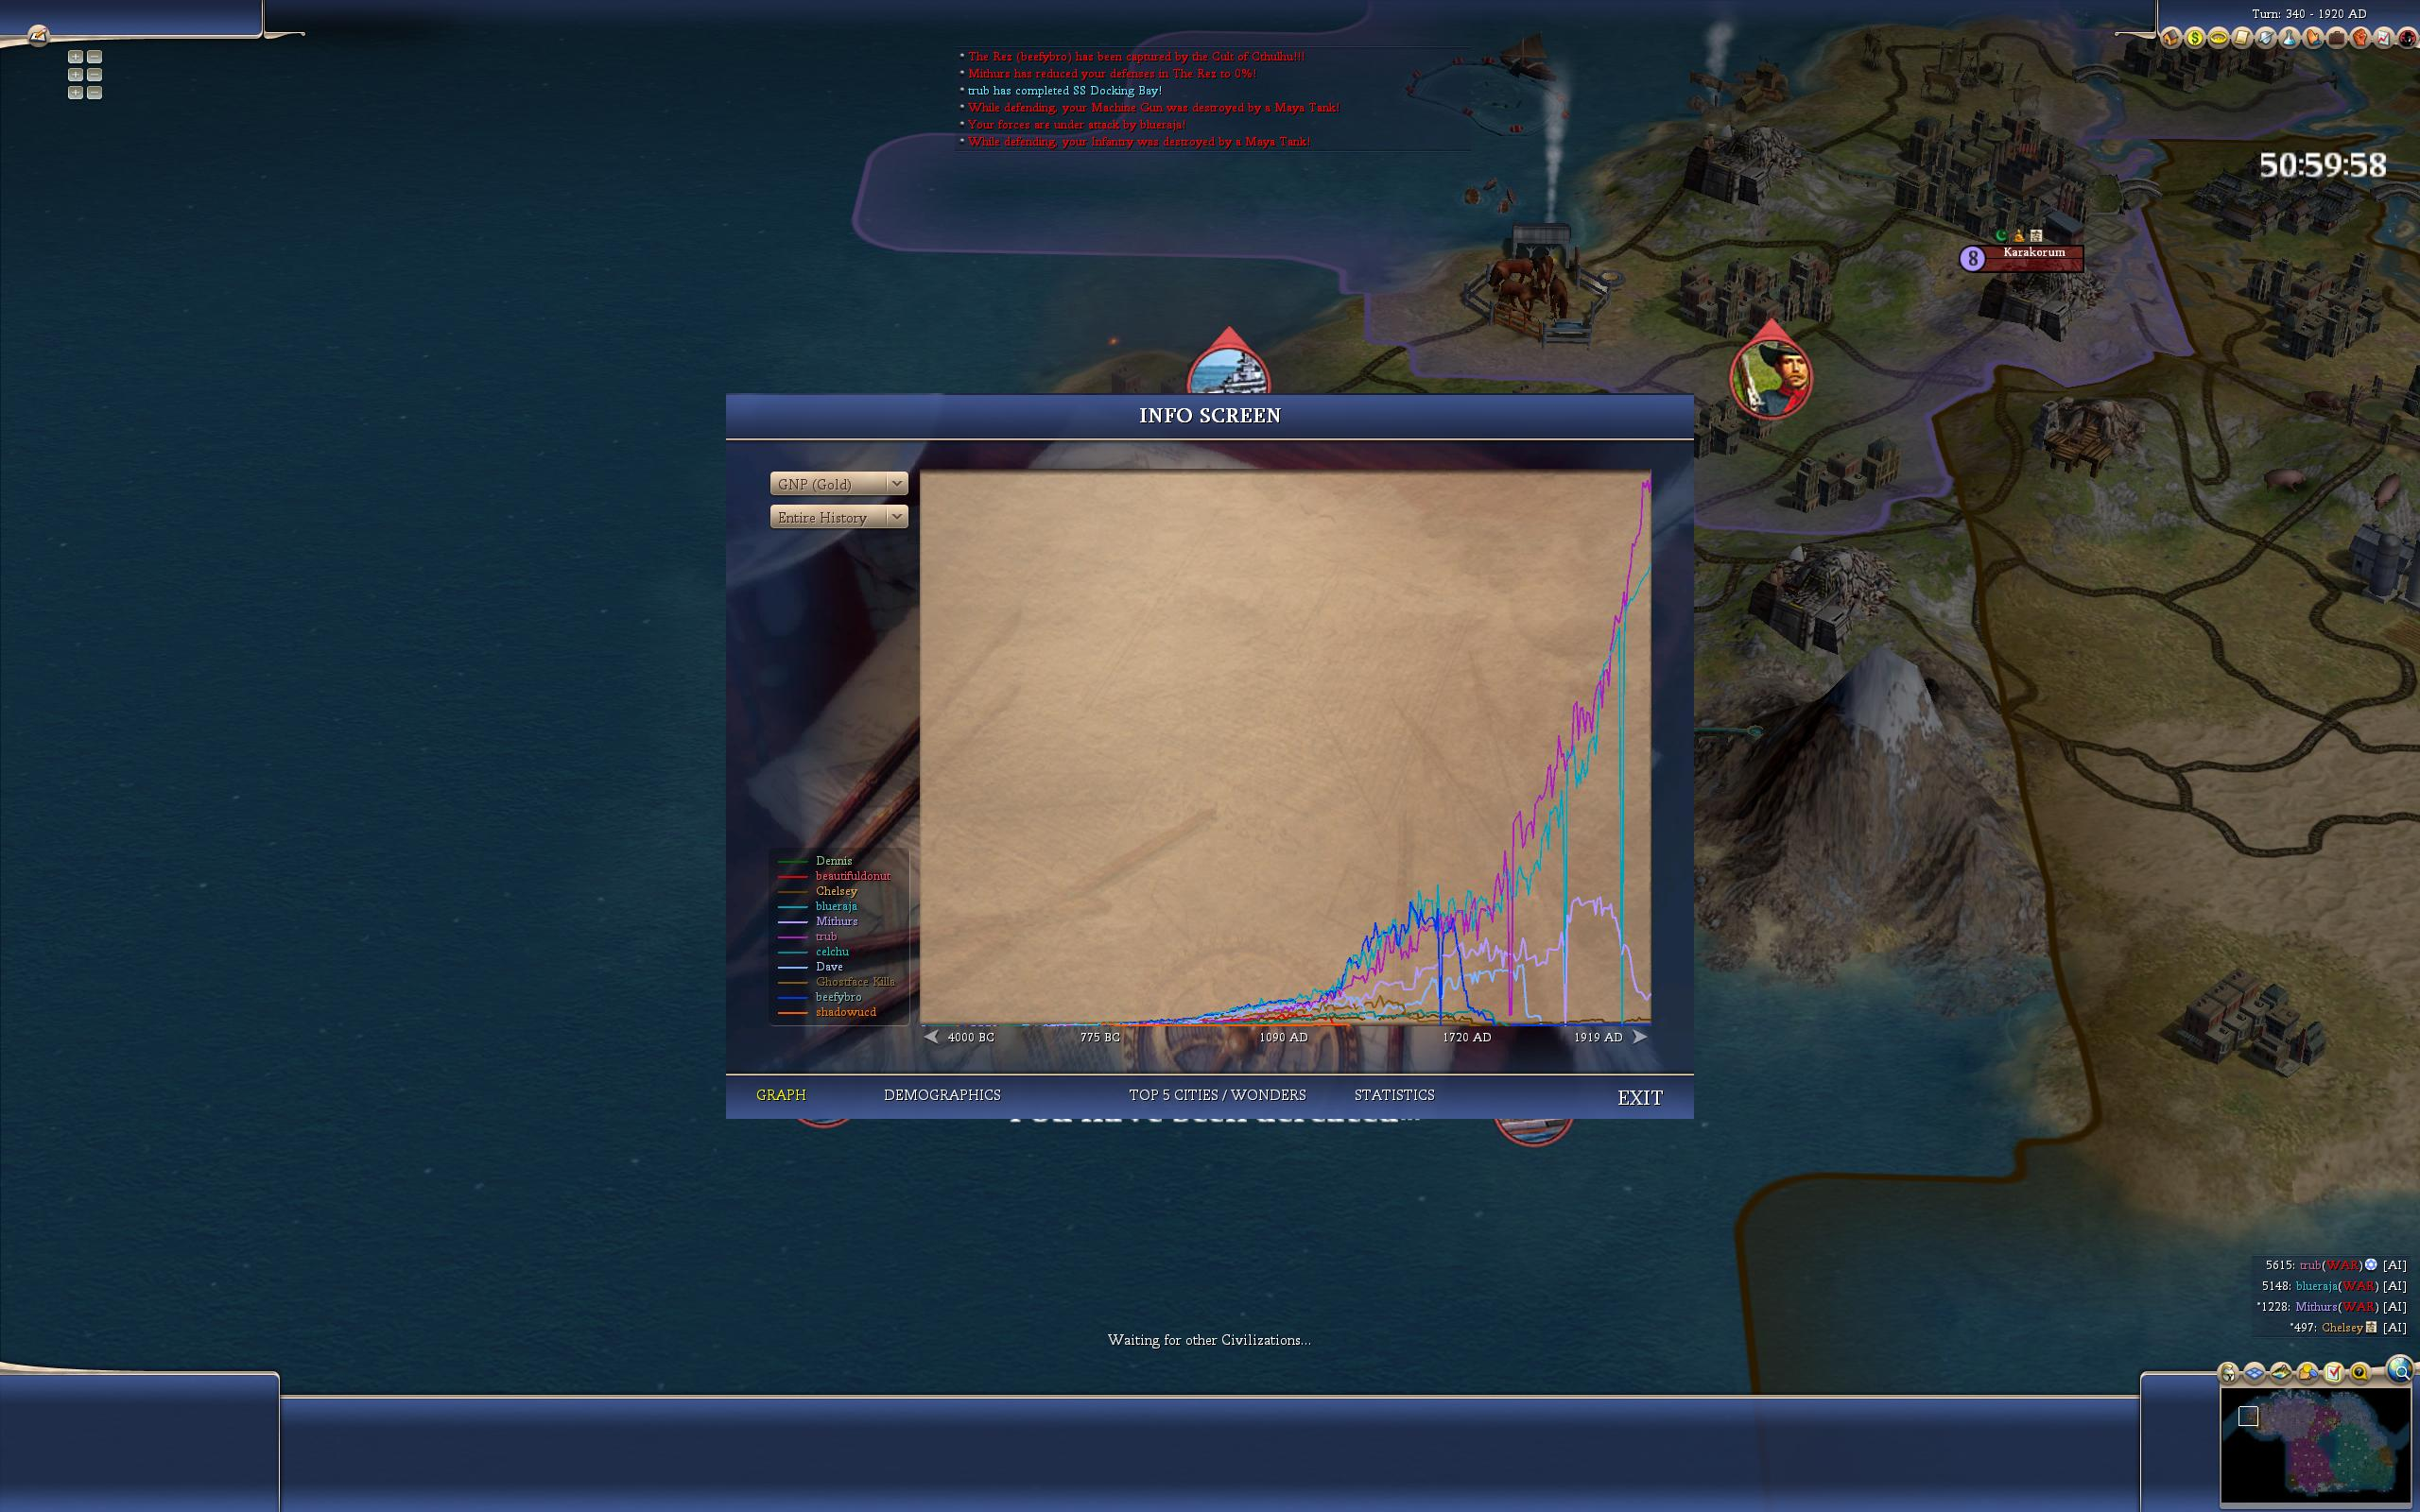
\includegraphics[width=1.0\textwidth]{end-2}
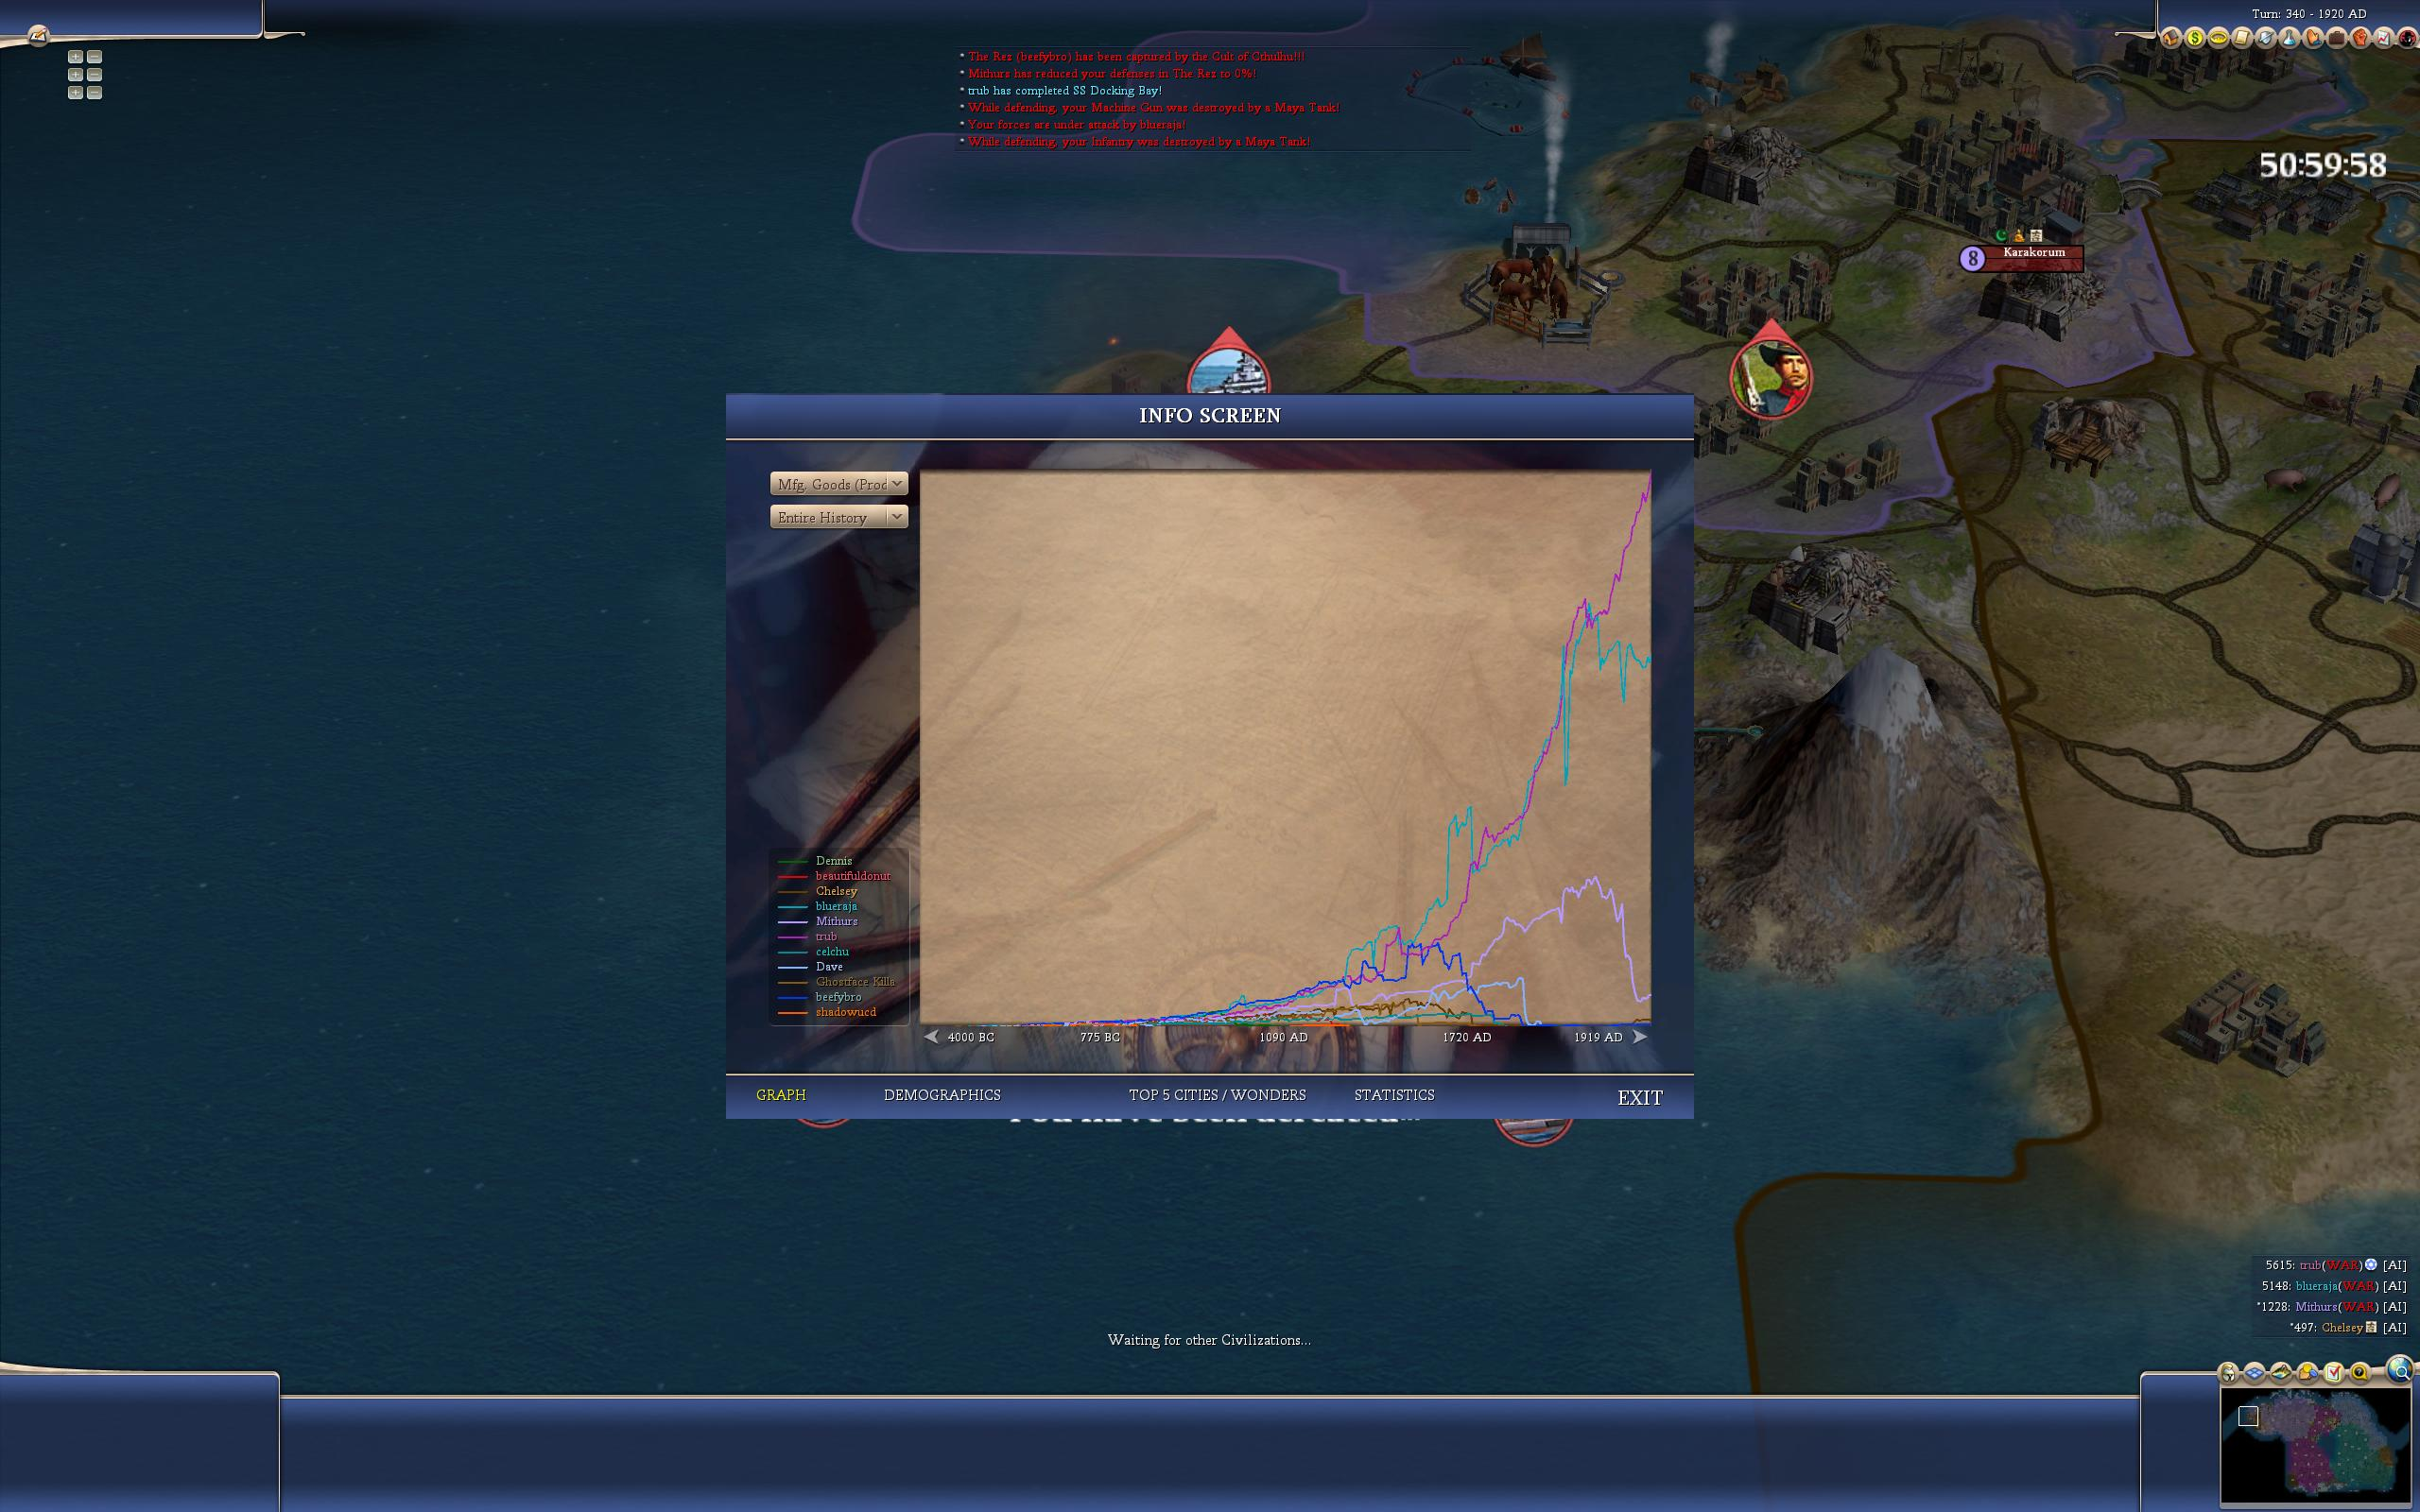
\includegraphics[width=1.0\textwidth]{end-3}
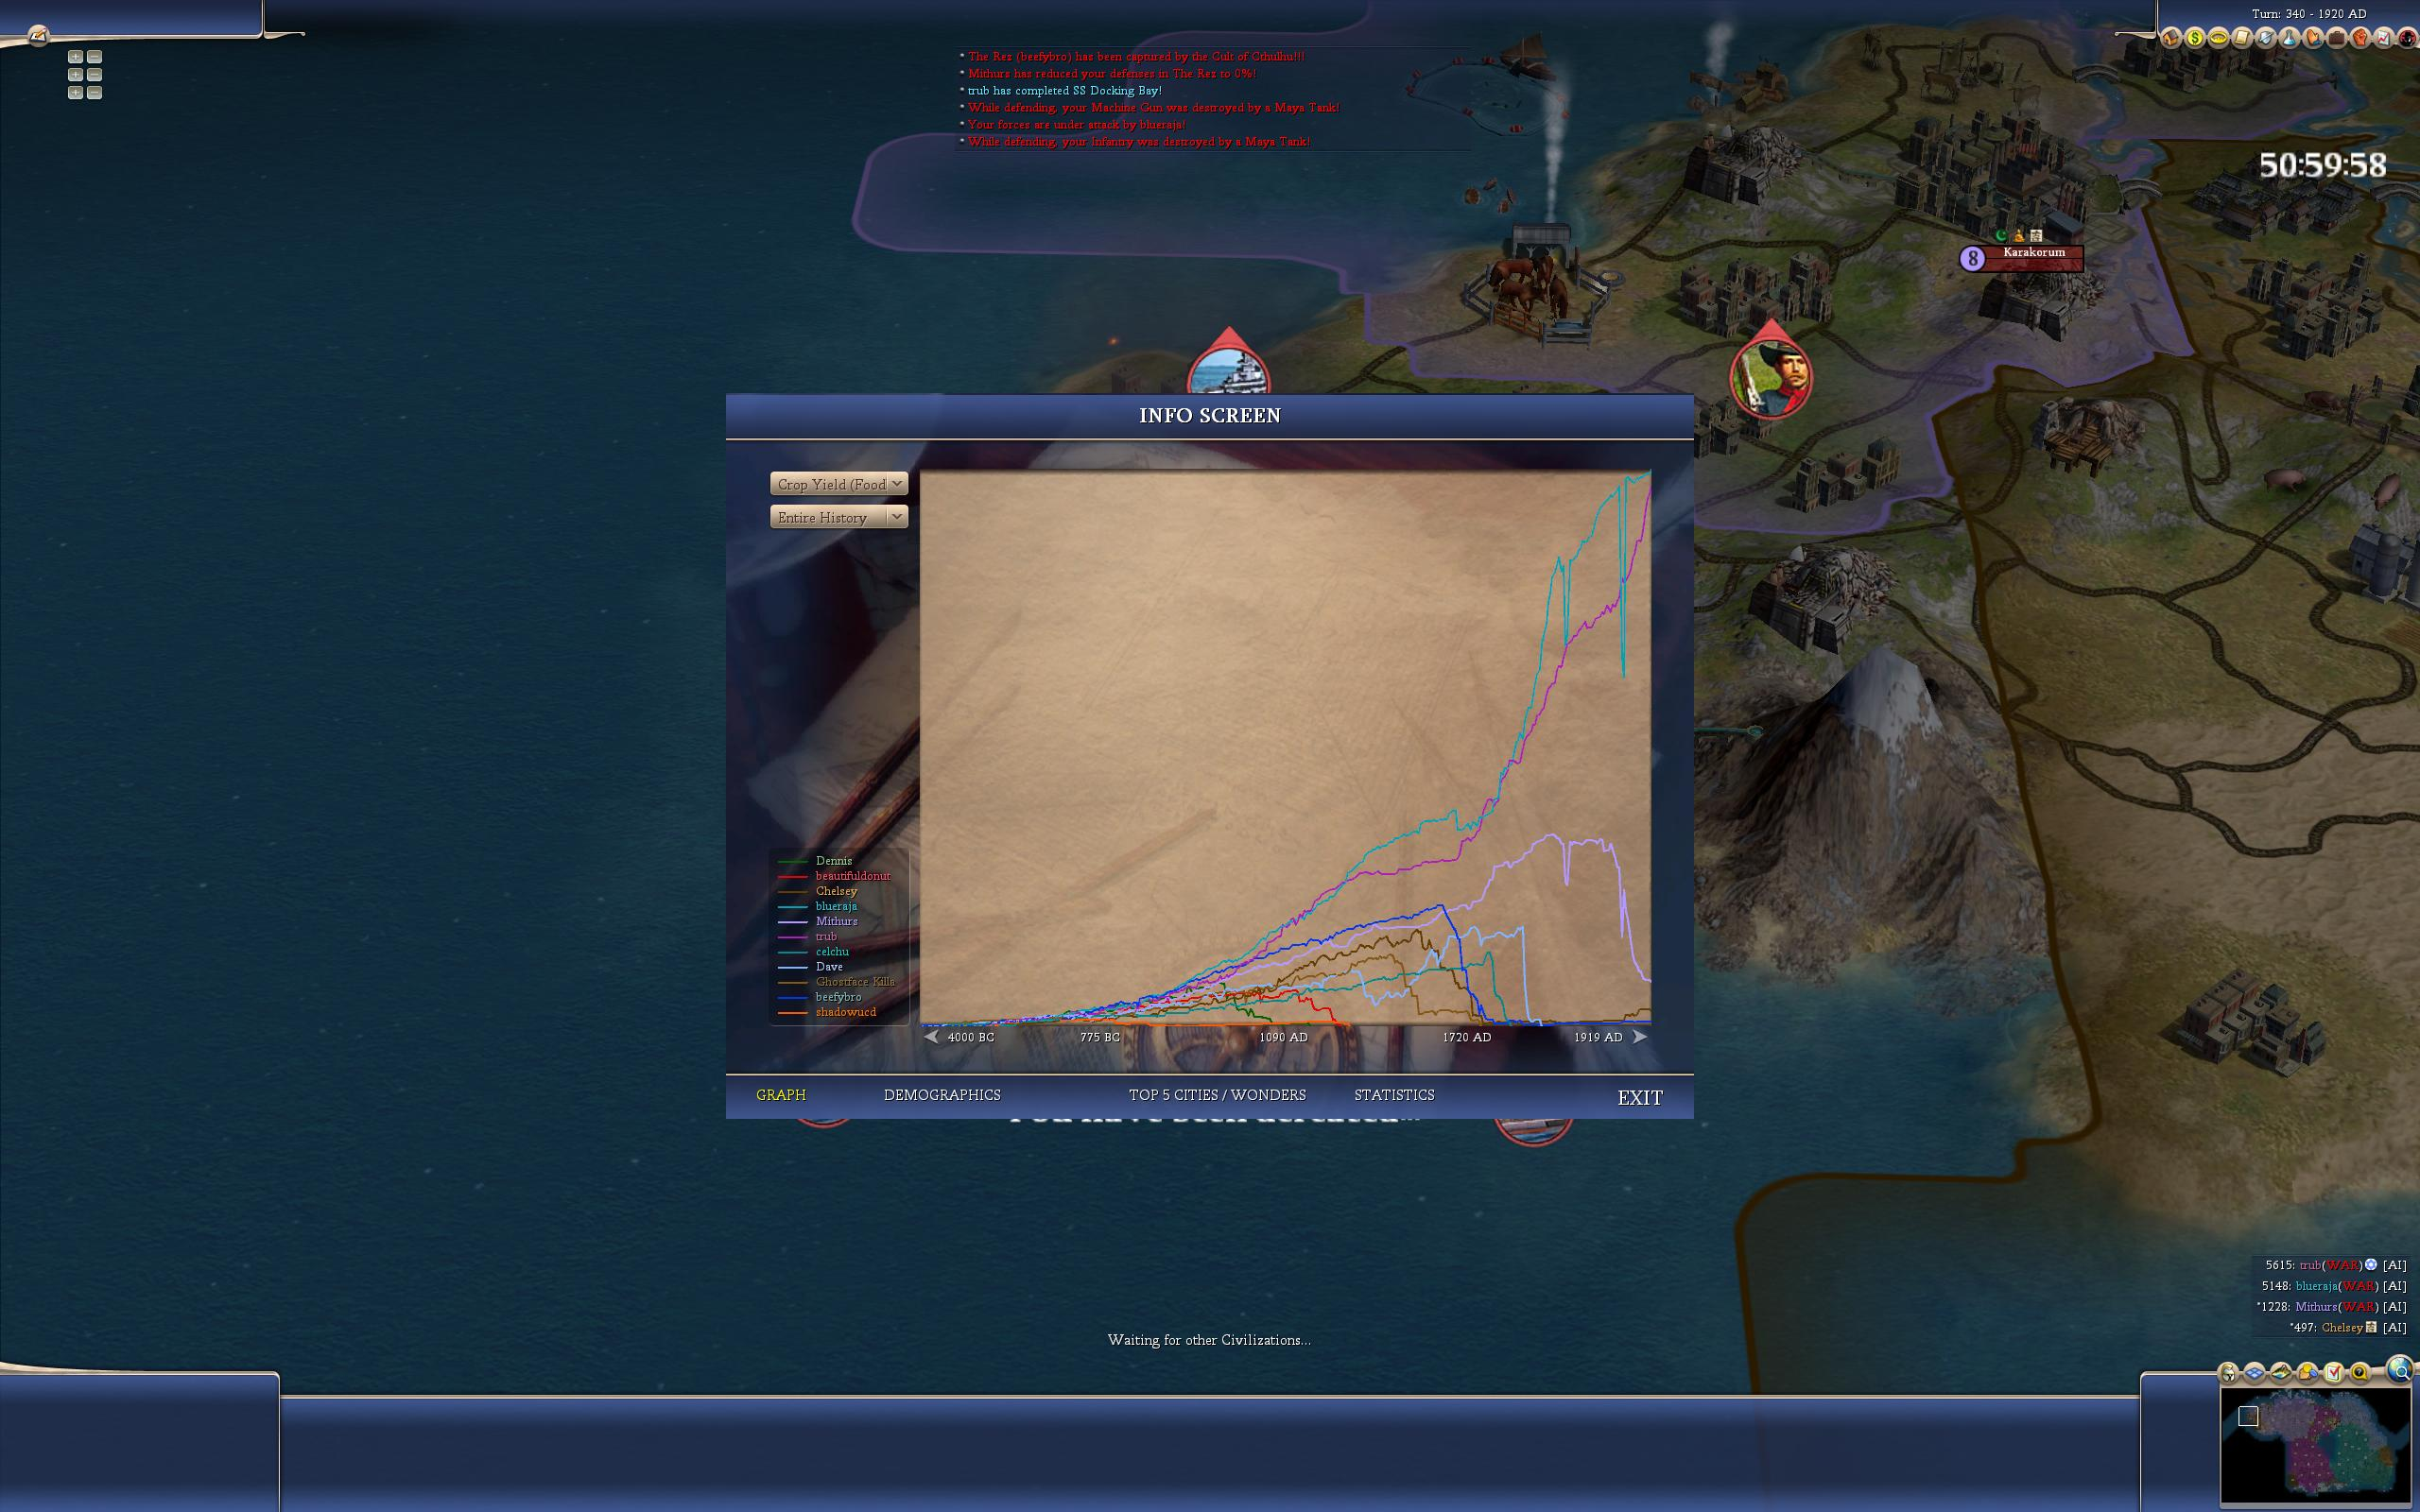
\includegraphics[width=1.0\textwidth]{end-4}
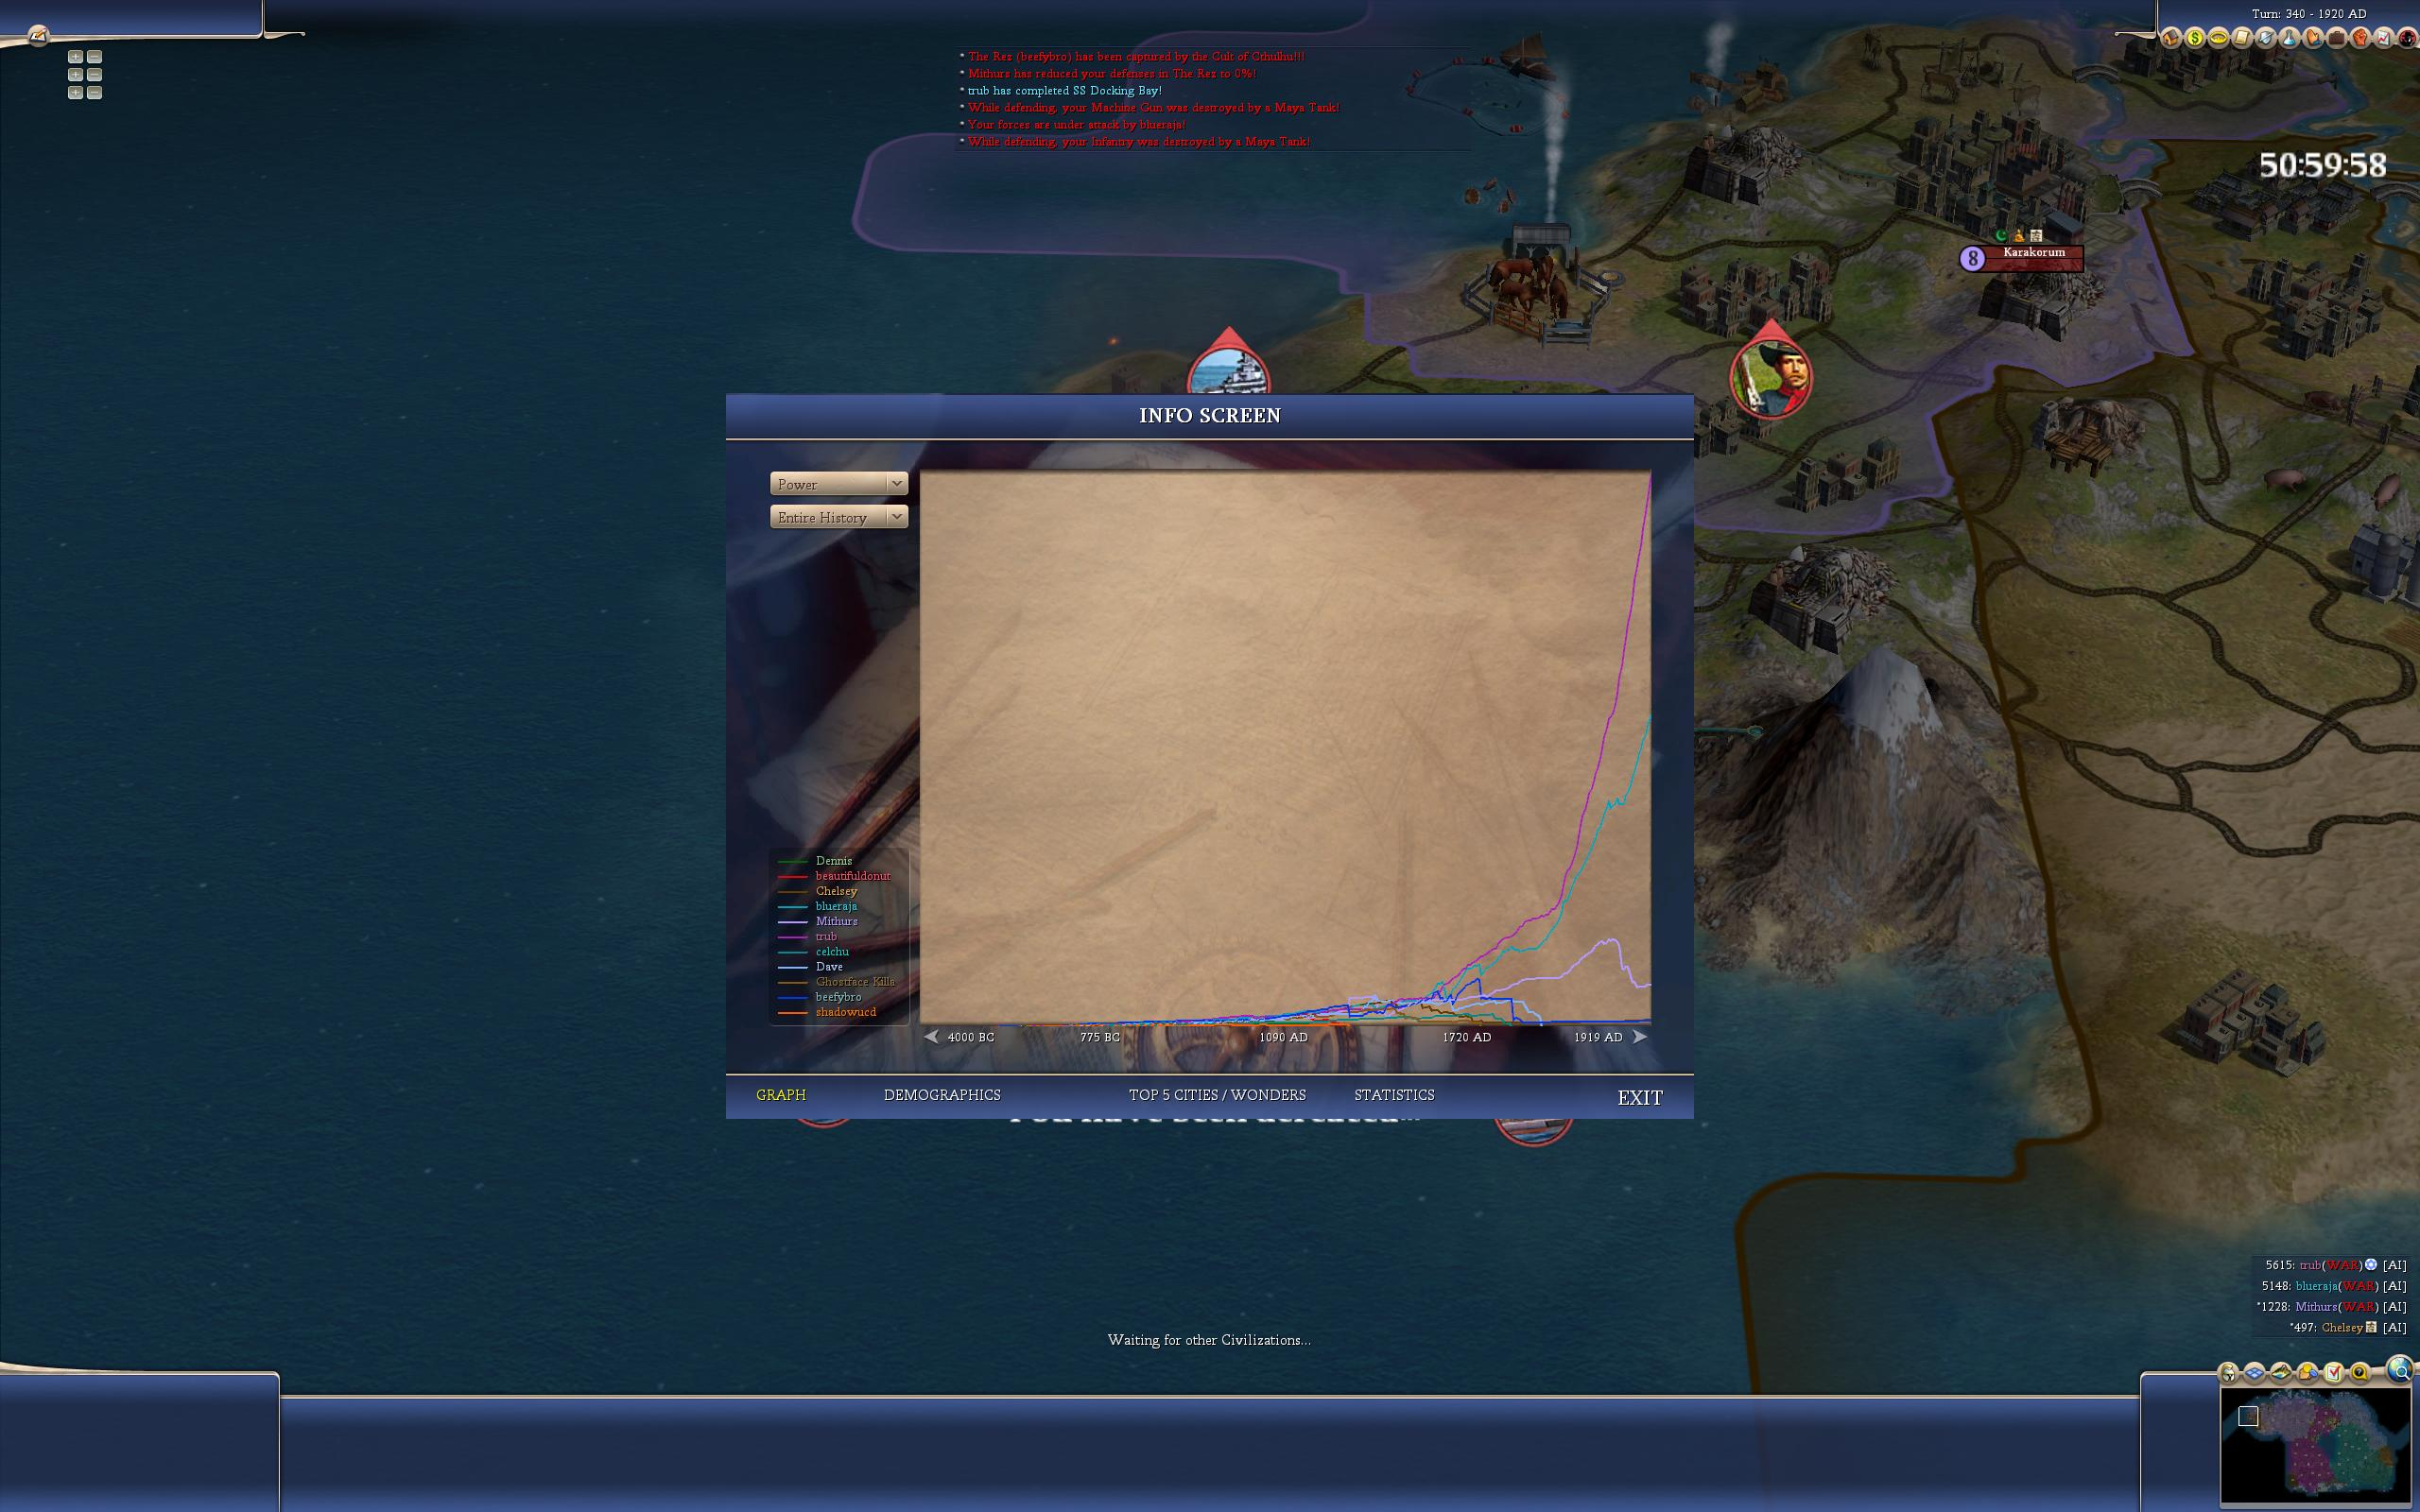
\includegraphics[width=1.0\textwidth]{end-5}
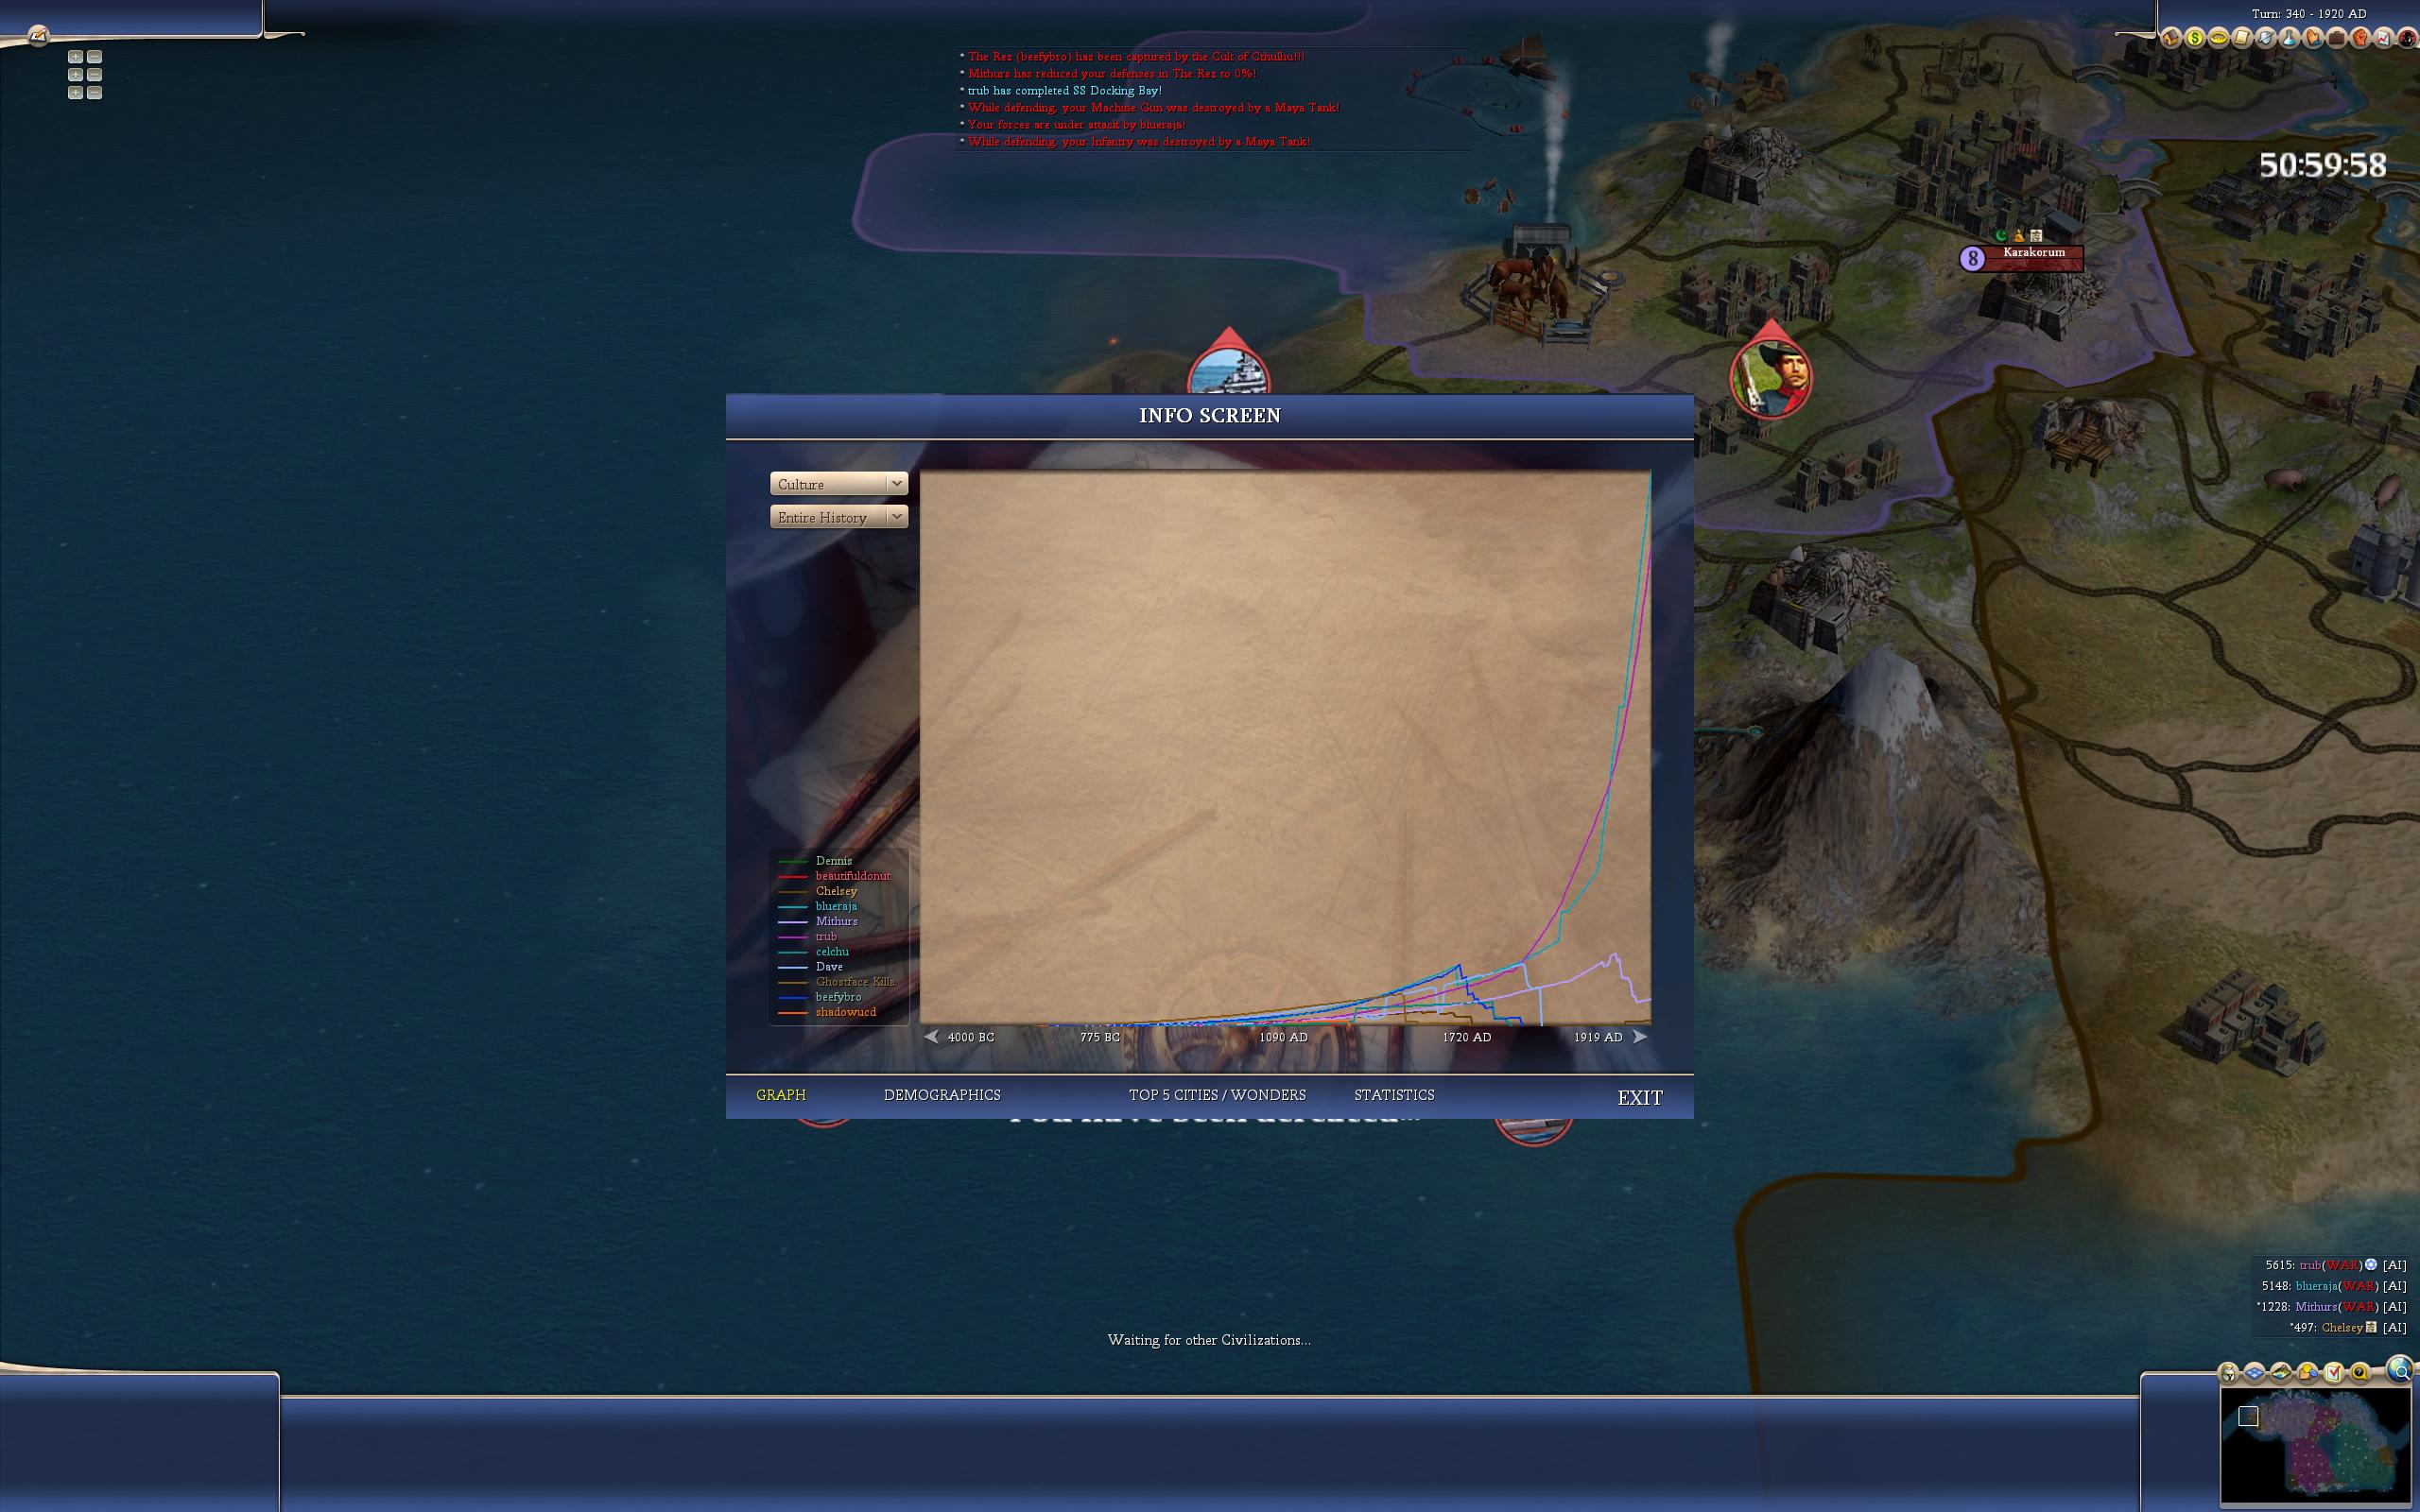
\includegraphics[width=1.0\textwidth]{end-6}
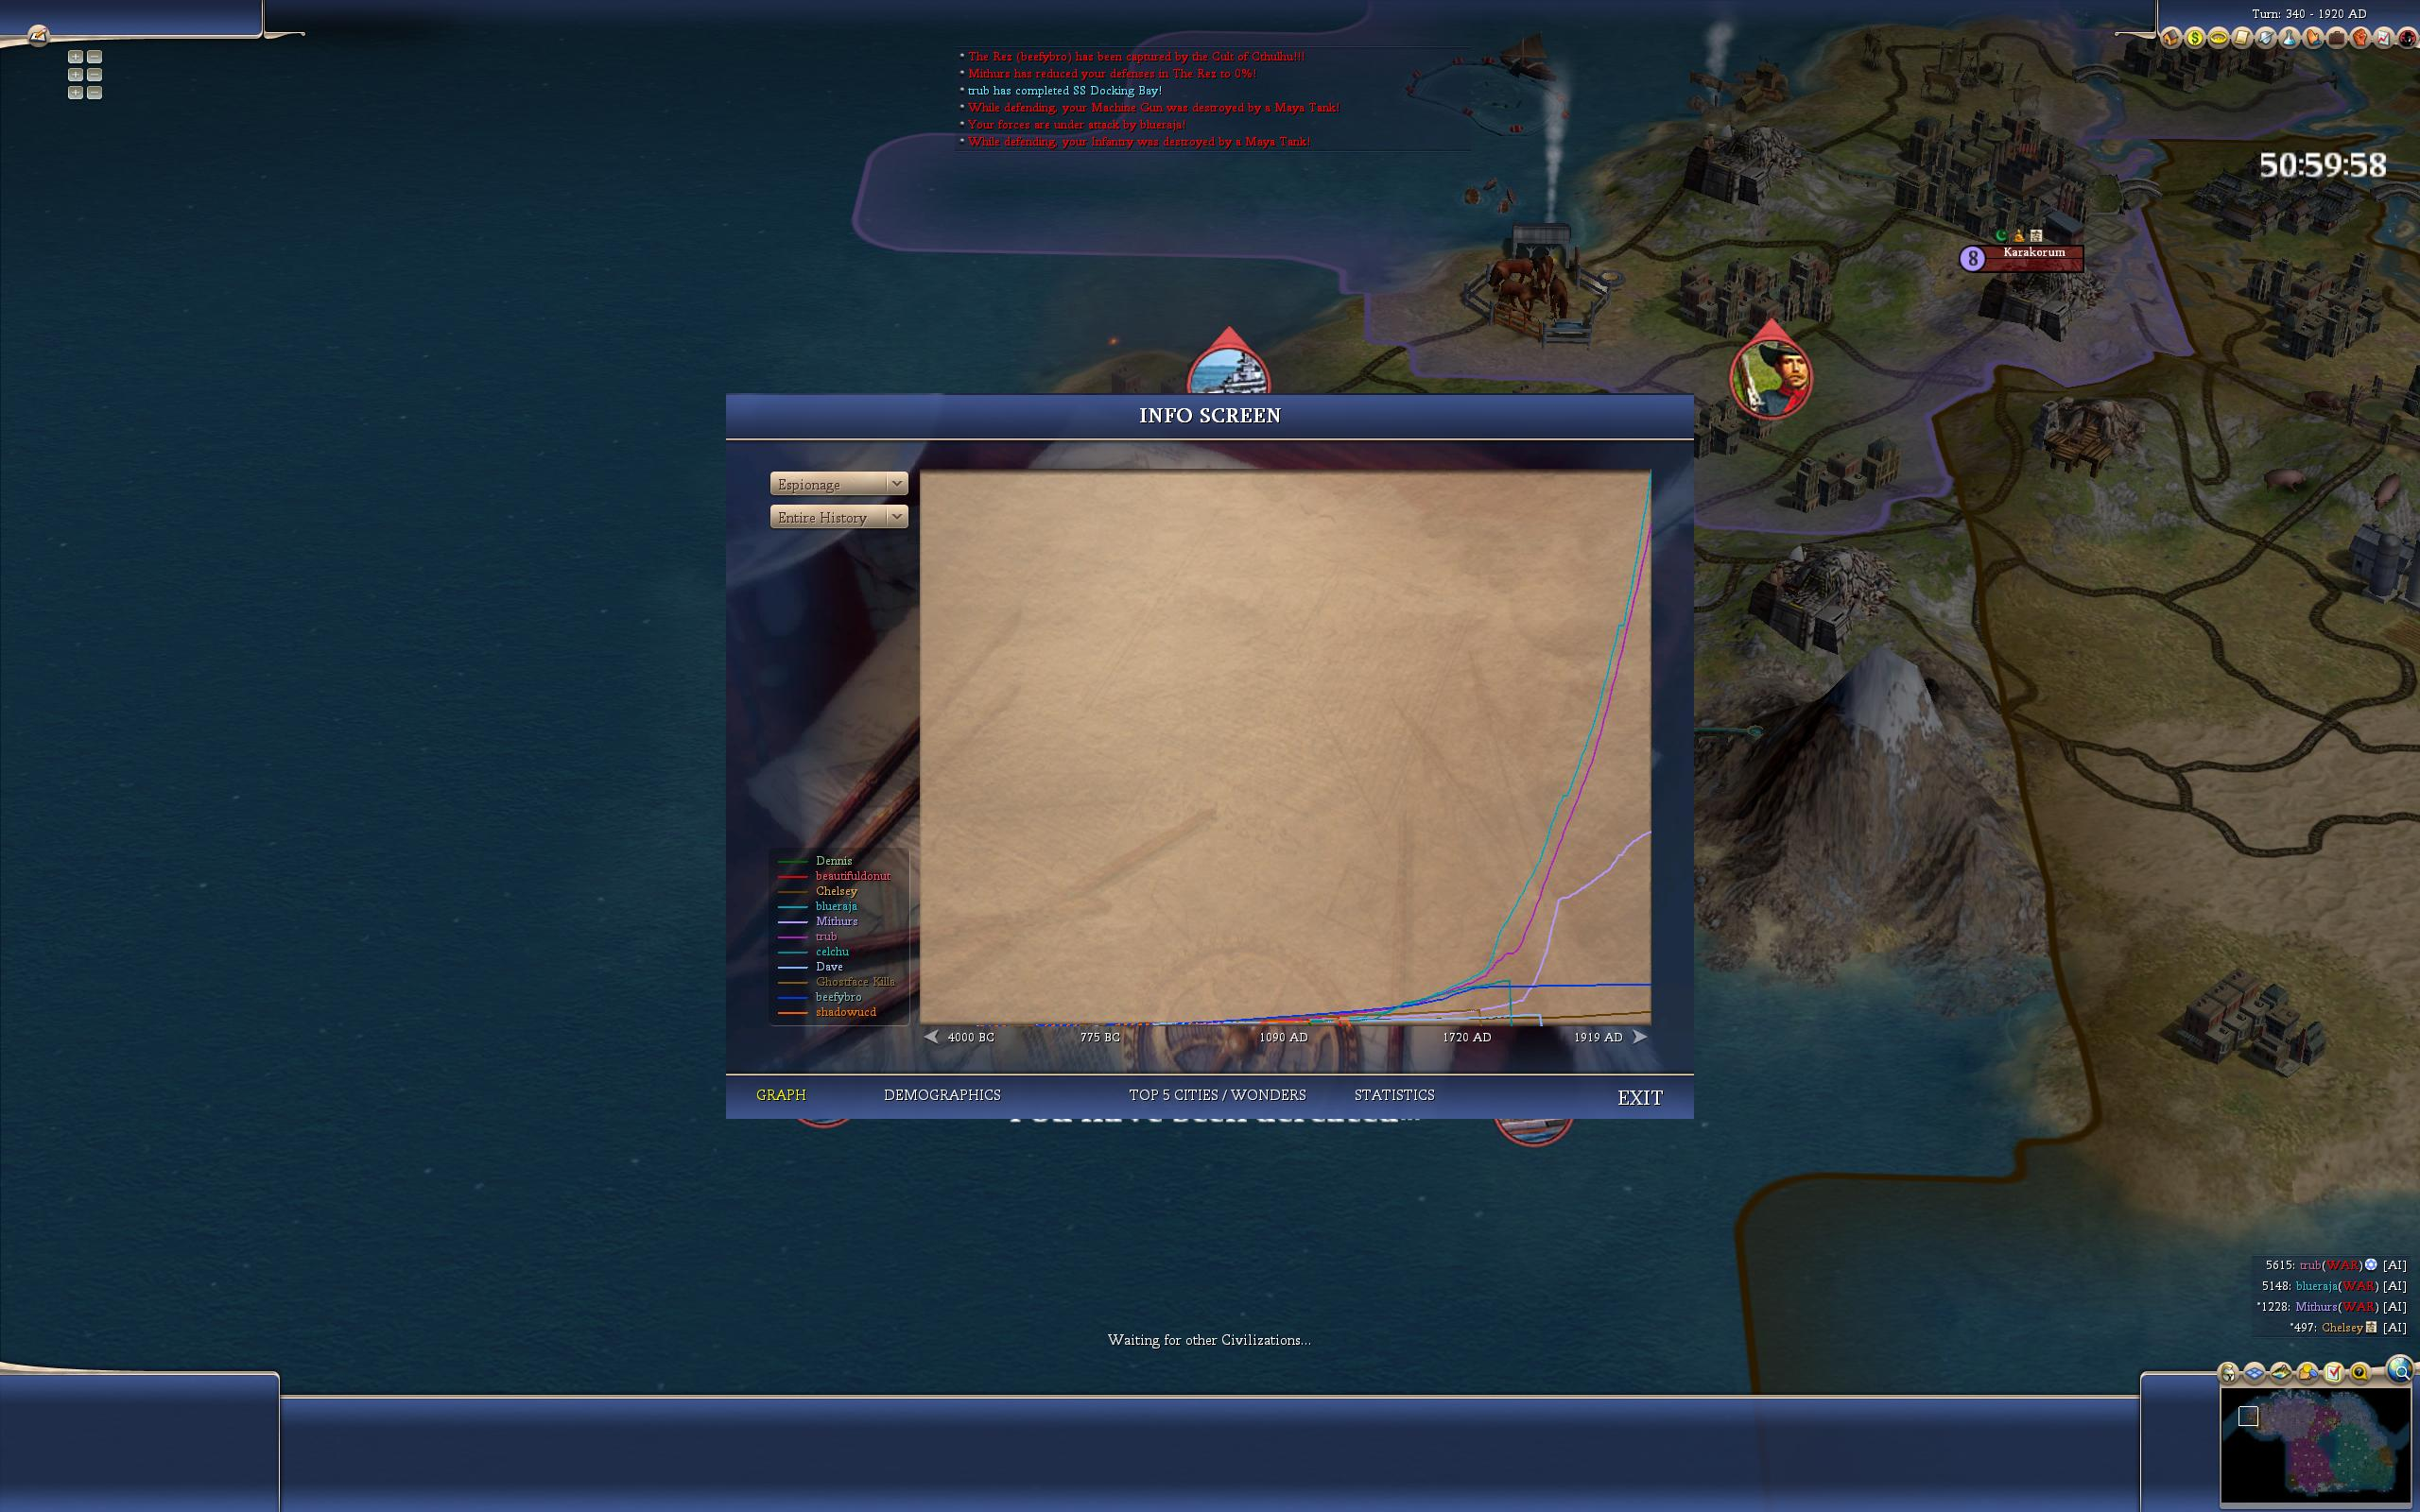
\includegraphics[width=1.0\textwidth]{end-7}



%Things to think about:
%* Once chopping starts, make sure city is growing while the worker is chopping and producing settler when the chop comes in.
%* During early game, if nothing all-that useful to produce, switch to scientist specialists (library)
%* Use demographics / scouting to look for incoming attacks
%* Every city should have at least one food resource
%* Pre-monarch, use slavery to whip unhappy cities
%* Switch to slavery ASAP
%* Lots of workers is good
%* Archery needs to come very early, don't even bother with warriors
%* Scouts should *always* run from bears
%* Scouts should *always* end their turn on forest or hill, preferably forest, forested hill even better.
%* keep city specialization in mind
%* Early focus must be on getting copper, ivory, iron, and horses.
%* Always produce the defender of a settler before the settler and have him start moving before the settler is out.
%* Aggressively switch to scientists when there is nothing too urgent to build.
% - Micro citizen placement intensely

\end{document}
